\documentclass[11pt,letterpaper]{report}
\usepackage[utf8]{inputenc}
\usepackage[T1]{fontenc}
\usepackage{lmodern}
\usepackage[english]{babel}
\usepackage[letterpaper,margin=1in]{geometry}
\usepackage{amsmath,amssymb,amsthm,mathtools}
\usepackage{bm}
\usepackage{enumitem}
\usepackage{xcolor}
\usepackage{tikz}
\usetikzlibrary{arrows.meta,calc,decorations.pathmorphing,decorations.markings,patterns,3d,intersections}
\usepackage{titlesec}
\usepackage[colorlinks=true,linkcolor=blue!50!black,urlcolor=blue!50!black]{hyperref}
\allowdisplaybreaks
\setlength{\parindent}{0pt}
\setlength{\parskip}{0.5em}

% Chapters: "Chapter n. Title" in the style of the original "Tema n."
\titleformat{\chapter}[hang]{\Large\bfseries}{Chapter \thechapter.}{0.5em}{}
\titlespacing*{\chapter}{0pt}{0pt}{1.5em}
% Sections: plain "n.m Title." as in the original
\titleformat{\section}[hang]{\normalfont\large}{\thesection}{0.5em}{}
\titleformat{\subsection}[hang]{\normalfont\itshape}{\thesubsection}{0.5em}{}
% Equations numbered (1), (2), ... restarting in every chapter, as in the original
\counterwithin*{equation}{chapter}
\renewcommand{\theequation}{\arabic{equation}}

% Bullet style of the original notes (small black squares)
\setlist[itemize,1]{label=\raisebox{0.15ex}{\tiny$\blacksquare$},leftmargin=1.2em,itemsep=0.5em}
\newenvironment{points}{\begin{itemize}}{\end{itemize}}

\newcommand{\dd}{\mathrm{d}}
\newcommand{\R}{\mathbb{R}}

\title{\Huge\bfseries Gravitation\\[0.5em]\Large Lecture Notes (Chapters 1--6)\\[0.3em]\large English translation}
\date{Academic year 2025/2026}
\author{}

\begin{document}
\maketitle
\tableofcontents
\chapter*{Syllabus}
\addcontentsline{toc}{chapter}{Syllabus}

\hfill Academic year 2025/2026

\begin{center}\Large Gravitation\end{center}

\begin{enumerate}[label=\arabic*.,leftmargin=1.5em]
\item \textbf{Newtonian gravitation.}
  \begin{enumerate}[label=1.\arabic*.,leftmargin=2.5em,itemsep=0pt]
  \item Newton's law of universal gravitation.
  \item Limitations of Newtonian gravitation.
  \item Tidal forces.
  \end{enumerate}
\item \textbf{The equivalence principle.}
  \begin{enumerate}[label=2.\arabic*.,leftmargin=2.5em,itemsep=0pt]
  \item Gravitational mass and inertial mass. Active and passive gravitational mass.
  \item Gravitational forces and non-inertial forces.
  \item Galileo's equivalence principle.
  \item Einstein's equivalence principle: gravity and space-time geometry.
  \end{enumerate}
\item \textbf{Brief introduction to differential geometry.}
  \begin{enumerate}[label=3.\arabic*.,leftmargin=2.5em,itemsep=0pt]
  \item Differentiable manifold. Tensors and tensor fields. Forms.
  \item Lie derivative.
  \item Covariant derivative. Connections. Parallel transport.
  \item Curvature, torsion and non-metricity.
  \item Metric. Levi-Civita connection.
  \item Introductory tutorial to the xAct package for Mathematica.
  \end{enumerate}
\item \textbf{Matter in gravitational fields.}
  \begin{enumerate}[label=4.\arabic*.,leftmargin=2.5em,itemsep=0pt]
  \item Particle in a gravitational field.
  \item Locally inertial frames. Riemann normal coordinates.
  \item Geodesics. Proper time. Geodesic deviation equation.
  \item Symmetries. Killing vectors. Conserved quantities.
  \item Principle of general covariance. Electromagnetism in gravitational fields.
  \end{enumerate}
\item \textbf{Einstein's equations.}
  \begin{enumerate}[label=5.\arabic*.,leftmargin=2.5em,itemsep=0pt]
  \item Derivation of Einstein's equations. Einstein--Hilbert action.
  \item Gravity as an interaction mediated by a massless spin-2 particle. Coupling to matter. The equivalence principle as a consistency condition.
  \item Vacuum solutions. Maximally symmetric spaces.
  \item Cosmological solutions: Friedmann--Lemaître--Robertson--Walker metrics.
  \item Spherically symmetric solutions: Schwarzschild metric and black holes.
  \item Orbits in Schwarzschild: null and timelike geodesics. Classical tests of Einstein's equations.
  \end{enumerate}
\item \textbf{Gravitational waves.}
  \begin{enumerate}[label=6.\arabic*.,leftmargin=2.5em,itemsep=0pt]
  \item Linearisation of Einstein's equations.
  \item Gauge invariance.
  \item Emission of gravitational waves: the quadrupole radiation formula.
  \item Detection of gravitational waves: interferometers.
  \end{enumerate}
\end{enumerate}

\section*{Bibliography}
\begin{itemize}[label={},leftmargin=0pt,itemsep=0.6em]
\item Misner, Thorne and Wheeler, ``Gravitation'', Freeman, 1973.\\
This book contains a vast amount of information and is extremely useful as a reference book, but it is perhaps not the best option for a first approach to the subject.
\item Sean Carroll, ``Spacetime and Geometry: An Introduction to General Relativity'', Addison Wesley, 2004.\\
This book is shorter and more accessible, while still being complete. It is a good reference for a first approach. There is a set of lecture notes by Eugene Lim based on this book (E.~Lim was a PhD student of Sean Carroll).
\item James Hartle, ``Gravity: An Introduction to Einstein's General Relativity'', Pearson, 2002.\\
This book makes extensive use of physical intuition and introduces many of the concepts and developments from a more physical point of view. It is a highly recommended book.
\item Bernard Schutz, ``A First Course in General Relativity'', Cambridge University Press, 2009.\\
Another good book for a first approach to General Relativity. It starts from basic concepts of special relativity and then makes the step to general relativity in a very geometric but instructive way.
\item L.D.~Landau and E.M.~Lifshitz, ``The Classical Theory of Fields'' (Spanish edition: \emph{Teoría clásica de los campos}, second edition, Editorial Reverté, Barcelona, 1993).\\
As always, this is a book that is best read once one already has some familiarity with General Relativity. It also has a good number of solved exercises that are very illustrative and useful.
\item Robert Wald, ``General Relativity'', University of Chicago Press, Chicago, 1984.\\
Another of the great classics for studying General Relativity. A very formal and very rigorous book.
\item N.~Straumann, ``General Relativity. With Applications to Astrophysics'', Texts and Monographs in Physics, Springer, 2004.\\
This book is also very formal and requires being comfortable with a more advanced mathematical language.
\item Steven Weinberg, ``Gravitation and Cosmology: Principles and Applications of the General Theory of Relativity'', Wiley \& Sons, 1972.\\
This book approaches gravity in a way that differs from the more usual geometric treatments. Weinberg was one of the pioneers of quantum field theory and of the Standard Model of particle physics, and this shows in the exposition. It is highly recommended to study this book because it provides a very physical and complementary view.
\item Feynman Lectures on Gravitation, Addison-Wesley Publishing Company.\\
These lectures are also advisable reading, because Feynman was one of the pioneers of the formulation of General Relativity from a field-theory perspective. They may not be so useful for studying gravitation, but they are for seeing Feynman's perspective, which is always very enriching. For a more complete treatment, Weinberg is more advisable.
\item Michele Maggiore, ``Gravitational Waves'', Vol.~I.\\
This book is a treatise on the production, propagation and detection of gravitational waves. The first chapters treat the foundations of General Relativity in considerable detail. It has a good number of exercises and examples on gravitational waves that are very useful.
\item Ray D'Inverno, ``Introducing Einstein's Relativity'', Oxford University Press, 1992.
\item Eric Poisson, ``A Relativist's Toolkit: The Mathematics of Black-Hole Mechanics'', Cambridge University Press, 2004.
\item Eric Gourgoulhon, ``Special Relativity in General Frames'', Graduate Texts in Physics, Springer, 2013.
\end{itemize}
A couple of references for the differential geometry part:
\begin{itemize}[label={},leftmargin=0pt,itemsep=0.3em]
\item B.F.~Schutz, ``Geometrical Methods of Mathematical Physics'', Cambridge University Press, 1980.
\item Nakahara, ``Geometry, Topology and Physics'', Institute of Physics Publishing, IoP, 2003.
\item Y.~Choquet-Bruhat, C.~DeWitt-Morette, M.~Dillard-Bleick, ``Analysis, Manifolds and Physics'', Elsevier Science Publishing Company Inc., 1982.
\end{itemize}

In addition to the textbooks mentioned, a wide variety of lecture notes by professors who have taught General Relativity can be consulted. Among them, one can mention:
\begin{itemize}[itemsep=0.3em]
\item The lecture notes of Matthias Blau. An impressive compendium of General Relativity of more than 900 pages, where almost everything can be found with very clear explanations. It ranges from elementary concepts to very advanced topics, so it is suitable for all audiences.
\item The notes of Daniel Baumann are very didactic and easy to follow. Moreover, they are fairly short ($\sim100$ pages).
\item Bert Janssen, of the University of Granada, has written these General Relativity notes, which can serve as a very good guide for the course because their table of contents is quite similar to the syllabus.
\item These notes by Luis Garay, of the Complutense University of Madrid, are very good and contain very interesting material. However, they are more useful for seeing some extensions of what is covered in class than for following the course syllabus.
\end{itemize}

\chapter{Newtonian gravitation}

\section{Newton's law of universal gravitation.}

\begin{points}
\item Newton's law of universal gravitation first appeared in the book ``Philosophiae Naturalis Principia Mathematica'' in 1687. It states that two masses exert on each other an attractive force along the straight line joining them, directly proportional to their masses and inversely proportional to the square of the distance:
\begin{gather*}
  F_g(1\to2)=-G\frac{m_1m_2}{r^2}e_r,\qquad e_r\ \text{unit vector pointing from particle 1 to particle 2},\\
  G\ \text{Newton's gravitational constant},\qquad G=6.674\cdot10^{-11}\,\frac{N\,m^2}{kg^2}.
\end{gather*}

\item When Newton presented it at the Royal Society of London in 1686, Robert Hooke accused him of having plagiarised his own ideas about the inverse-square dependence on distance. In fact, in his ``Principia'' Newton explicitly mentioned that the idea that the force between the Sun and the planets might be inversely proportional to their mutual distance had been proposed by Hooke, as well as by Sir Christopher Wren and by Edmund Halley, with whom he had corresponded on the subject (for instance, in 1679 Hooke wrote to Newton communicating his idea of the inverse-square dependence on distance). He also mentioned Ismaël Bullialdus, a French astronomer and mathematician of the time who had already proposed the inverse-square law of proportionality in 1645. However, Bullialdus did not accept Kepler's second and third laws and, in fact, in his theory the force exerted by the Sun on the planets was attractive at aphelion and repulsive at perihelion.

\item The fundamental difference between Newton's proposal and all the previous ones is that Newton justified his proposal by studying its consequences. For example, he derived Kepler's laws and proved that for spherical bodies the gravitational field was independent of the size of the object, thereby justifying that the law could be applied near the surface of the Earth, in a regime in which the Earth obviously cannot be treated as a point particle.

\item A fundamental component of Newton's law of gravitation is that it is universal, i.e.\ it applies to all bodies, both on Earth and in the heavens.

\item According to the famous story of Newton and the apple, which has reached us through the writings of John Conduitt (who was Newton's assistant at the Royal Mint and the husband of his niece), in 1666 Newton came up with the idea that the action of gravity, which acted on everyday objects (for instance making apples fall from a tree), might also act at distances much greater than was normally thought, so that it might act on the Moon and be the cause of it remaining in orbit around the Earth.

\item Note that the date in this account, 1666, is much earlier than the publication date of the Principia. The fact is that the idea that gravitation could be a universal phenomenon was already mature enough at that time for more than one scientist to propose it. For example, Hooke himself had published in 1674 a work that aimed to explain a ``System of the World'' based on three hypotheses: 1) all celestial bodies undergo an attraction towards their own centres, 2) they also attract all the other celestial bodies that lie within their sphere of attraction, and 3) any body set in simple and direct motion will keep moving forward in a straight line until it is deflected by other ``effective powers''. Hooke's version is not completely universal, but it already comes very close.

\item The universal gravitational constant $G$ was measured for the first time by Sir Henry Cavendish in a work published by the Royal Society of London in 1798, in which he described his experiment based on a torsion balance. It is worth noting that Cavendish's primary goal was not to measure $G$ (he does not even mention it in his article) but to obtain the mean density of the Earth (Cavendish concludes that the Earth is 5.48 times denser than water). Measuring the density of the Earth is equivalent to knowing its mass. Combining this datum with the value of the intensity of the gravitational force at the surface of the Earth (approximately $g=9.81\,\mathrm{ms^{-2}}$), one obtains the value of $G$ from the expression $g=\frac{GM}{R^2}$, where $R$ is the radius of the Earth.

\item All the gravitational physics developed in the eighteenth and nineteenth centuries (and a good part of the research carried out in the twentieth and twenty-first centuries) is based on the law of universal gravitation combined with the superposition principle, which states that the total gravitational force on a body is the sum of the individual (gravitational) forces exerted by each of the objects that make up the system.

\item These two laws lead immediately to Poisson's law for the gravitational potential.

\item The force of universal gravitation is conservative, $F=-\nabla U=-m\nabla\Phi$, with the gravitational potential (per unit mass) $\Phi$ given by
\[
  \Phi=-G\frac{m_1}{r}
\]
as follows directly from $\nabla\frac1r=-\frac{1}{r^2}e_r$.

\item The gravitational potential generated by a continuous, compactly supported mass distribution described by a mass density $\mu(x)$ is
\[
  \Phi(x)=-\int_VG\frac{\mu(y)}{|x-y|}dy
\]
where $V$ is the volume in which the mass density does not vanish. If we compute the Laplacian of $\Phi$ we obtain
\begin{equation}
  \Delta\Phi=4\pi G\mu .
\end{equation}
This equation can be derived using the fact that, in the sense of distributions, $\Delta_x|x-y|^{-1}=-4\pi\delta(x-y)$, where $\delta(a)$ is the Dirac distribution centred at the point $a$.

\item This equation is called \emph{Poisson's equation} and, when supplemented with suitable boundary data, it provides the gravitational potential generated by a mass distribution $\mu$. For example, when the distribution has compact support, the boundary condition is $\Phi(|x|)\to0$ as $|x|\to\infty$.

\item When one considers a number $n$ of spatial dimensions different from 3, the fundamental equation of the gravitational field is still Poisson's equation.

\item We must decide whether to keep the number $4\pi$ appearing in Poisson's equation or to replace it by another quantity. The change would only amount to a redefinition of $G$, so there is no loss of generality in keeping the form (1) (this choice seems to be the most common one in the literature, but it is not the only one).

\item We can define the Green's function $G(x;y)$ as the general solution of the distributional equation
\[
  \Delta_xG(x;y)=-\delta(x-y)
\]
that satisfies the following condition: in dimension $n=2$ it must depend only on $x-y$, and in dimension $\geq3$ it must satisfy $G(x;y)\to0$ as $|x|\to\infty$ with $y$ fixed.

\item One can show that the Green's function takes the form
\[
  G(x;y)=\left\{\begin{array}{ll}-\frac{1}{2\pi}\log(|x-y|)+C, & n=2,\\[0.5ex] \frac{1}{(n-2)\omega_{n-1}}\frac{1}{|x-y|^{n-2}} & n\geq3,\end{array}\right.
\]
where $\omega_{n-1}$ is the area of the sphere of unit radius in $\R^n$ and $C$ is an arbitrary constant. Since the potential is always defined up to an arbitrary constant, we can choose $C=0$ without loss of generality.

\item We conclude that the gravitational field of a point mass located at the point $y$ in a Euclidean space of dimension $n\geq2$ is
\begin{align*}
  \Phi(x)&=-4\pi G\frac{m}{(n-2)\omega_{n-1}}\frac{1}{|x-y|^{n-2}}, && n\geq3,\\
  \Phi(x)&=2Gm\log(|x-y|), && n=2.
\end{align*}
Note that in dimension 2 the gravitational potential tends to infinity as the distance between the particles tends to infinity. The force, however, decreases as the inverse of the distance and therefore vanishes at infinity.
\end{points}

\section{Successes and limitations of the theory.}

\begin{points}
\item Let us place ourselves at the beginning of the twentieth century. While electromagnetic theory had advanced enormously during the nineteenth century, with the works of Ampère, Ohm, Biot and especially of Faraday and Maxwell, culminating in Maxwell's equations, the theory of gravitation had remained unchanged in its basic aspects since its formulation by Newton.

\item The fundamental idea of Newtonian gravitation is that massive particles interact through an action at a distance between them, i.e.\ masses attract each other instantaneously and without the need for any mediation between them. Of course, one can reformulate Newtonian gravitation and introduce a gravitational field $\Phi(x,t)$, but this field changes instantaneously when we modify the configuration of the masses.

\item In this sense one cannot say that this field has an independent existence, as can be asserted in the case of the electromagnetic field, since the latter can propagate in the form of radiation and be measured.

\item For a physicist of the early twentieth century this instantaneous action at a distance could seem strange compared with the propagation at finite speed of electromagnetic waves, but it was not necessarily in contradiction with his physical conceptions, since the framework in which he worked was that of Galilean relativity and, in particular, of the existence of an absolute, universal and observer-independent time.

\item This perception changed radically in 1905 with the development of Einstein's special relativity. This theory predicts, among other things, that time is not absolute but depends on the observer. In other words, distinct events that are simultaneous for an observer in an inertial frame need not be so for another observer moving with constant velocity with respect to the former.

\item Consequently, the concept of instantaneous action at a distance is incompatible with special relativity, since the interaction could only be instantaneous for one inertial observer. The latter would automatically become a privileged observer, which would contradict the principle of relativity.

\item Although the theory of special relativity needed some time to be accepted, already in 1906 Henri Poincaré pointed out that the Newtonian theory of gravitation is incompatible with special relativity. It was clear (especially from our modern perspective, in which special relativity is a physical theory fully confirmed from an experimental point of view) that it was necessary to modify the Newtonian theory of gravitation.

\item However, this was a purely theoretical need for consistency. On the other hand, in the last instance physics must always be based on observations. It is therefore legitimate to ask whether, at the end of the nineteenth or the beginning of the twentieth century, there was any experiment or observation of a gravitational nature that could not be satisfactorily explained by Newtonian gravitation.

\item It is worth stressing that the planet Neptune was discovered in 1846 by the astronomer Johann G.~Galle, of the Berlin Observatory, on the basis of some calculations carried out by the French mathematician Urbain Le Verrier, who told him in which part of the sky he should look.

\item The basis of this discovery lies in the fact that the planet Uranus did not follow the trajectory predicted by Newtonian gravitation when all the corrections due to the effect of the planets known at that time were taken into account. In 1842 the Göttingen Academy of Sciences offered a prize to whoever solved the problem of Uranus.

\item Le Verrier assumed that the discrepancy in the motion of Uranus was due to the existence of a more distant planet, of undetermined mass and position. Through a perturbative calculation of the planetary orbits and its comparison with the actual data on the motion of Uranus, Le Verrier was able to predict the position of Neptune and communicate it to Galle.

\item It is curious to note that the solution to this problem had been found earlier, by the same method, by a recent graduate of the University of Cambridge, John C.~Adams, who in 1843 found the solution and asked the Astronomer Royal George B.~Airy to observe that position in the sky. Unfortunately, Airy paid no attention whatsoever. It was not until 1848 that Adams was given the credit he deserved; in that same year he was awarded the same prize that had been awarded to Le Verrier the previous year.

\item We see, therefore, that Newtonian theory was precise enough to predict the motion of Uranus with such accuracy that the discrepancy with the observations could be resolved with the discovery of another planet.

\item In fact, all the astronomical predictions based on Newtonian gravitation agreed perfectly with the observations, with a single exception: the precession of the perihelion of Mercury.

\item Recall that, to solve the problem of two isolated bodies in Newtonian mechanics, one introduces a variable $\vec r:=\vec r_2-\vec r_1$ for the position of the second body relative to the first, and a variable $\vec R_{CM}:=\frac1M(m_1\vec r_1+m_2\vec r_2)$, which gives the position of the centre of mass ($m_1$ and $m_2$ are the respective masses of particles 1 and 2 and $M:=m_1+m_2$ is the total mass of the system). If the interaction force between the two particles is $\vec f(\vec r)$ (more precisely, the force exerted by particle 1 on particle 2 is $\vec f$, and it depends only on $\vec r_2-\vec r_1$; we also assume that Newton's third law holds in the system), Newton's equations reduce to
\begin{gather*}
  M\frac{d^2\vec R_{CM}}{dt^2}=0,\\
  \mu\frac{d^2\vec r}{dt^2}=\vec f(\vec r)
\end{gather*}
where $\mu:=\frac{m_1m_2}{m_1+m_2}$ is the reduced mass of the system. If the interaction between the particles is gravitational we have
\[
  \vec f=-G\frac{m_1m_2}{r^2}e_r=-G\frac{\mu M}{r^2}e_r
\]
so that the relative position between the two masses satisfies the equation
\[
  \frac{d^2\vec r}{dt^2}=-G\frac{M}{r^2}e_r .
\]
Consequently, the motion of particle 2 relative to 1 is planar and, in polar coordinates $\{r,\phi\}$ centred at the position of 1, it follows the trajectory
\[
  \frac pr=1+\epsilon\cos(\phi-\phi_0)
\]
where $p$, $\phi_0$ and $\epsilon$ are constants. $p$ has dimensions of length (the so-called ``semi-latus rectum'') and $\epsilon\geq0$ is a dimensionless parameter called the eccentricity. When $\epsilon=1$ the orbit is a parabola, when $\epsilon>1$ the orbit is a hyperbola and when $0\leq\epsilon<1$ the orbit is an ellipse (which degenerates into a circle when $\epsilon=0$).

\item In the case $\epsilon<1$, the ellipse has its major axis along the line $\phi=\phi_0$, and the values of the semi-major and semi-minor axes are, respectively,
\[
  a=\frac{p}{1-\epsilon^2},\qquad b=\frac{p}{\sqrt{1-\epsilon^2}}
\]
and with principal axis along the line $\phi=\phi_0$.

\item In the inertial frame in which the centre of mass is at rest and located at the origin, the motion of each particle with respect to the origin is also an ellipse, with the same eccentricity $\epsilon$ and semi-major axis
\begin{align*}
  a_1&=\frac{m_2\,a}{m_1+m_2}, &&\text{particle 1},\\
  a_2&=\frac{m_1\,a}{m_1+m_2}, &&\text{particle 2}.
\end{align*}

\item The Solar System is made up of many bodies. However, for a given planet the main contribution to its motion is that of the Sun, and the effect of the other celestial bodies can be studied by means of perturbation theory.

\item The main effect of the perturbations is that the ellipse essentially keeps its shape but the orbit rotates around the Sun, in the same direction as the revolution of the planet or in the opposite direction, depending on the conditions.

\item In 1855 Urbain Le Verrier computed the theoretical precession of Mercury due to the effects of the other planets of the Solar System (essentially Venus, Earth, Jupiter and Saturn, which are the ones with the largest influence in this case).

\item He found that it should be 527 arcsec/century in the direction of motion. Using observations covering a period of a century and a half, Le Verrier also determined that Mercury precessed by 565 arcsec/century, so that there was a discrepancy of 38 arcsec/century.

\item As a possible explanation, Le Verrier proposed either the existence of a belt of planetoids between Mercury and the Sun, or the existence of a planet inside the orbit of Mercury.

\item Shortly after the publication of these results, in 1859, an amateur astronomer named Lescarbault announced that he had already observed a small planet in transit across the Sun, which was named Vulcan. Le Verrier considered this observation satisfactory. The Royal Society of London hailed the discovery as ``the second triumphant conclusion of the theoretical investigations of Monsieur Le Verrier''.

\item However, observing planets so close to the Sun is very difficult, so there was controversy about the actual existence of Vulcan. There were several announcements of other observations of Vulcan, although some of them proved to be false or mistaken. In 1876 Le Verrier predicted transits of Vulcan that could be observed. Le Verrier died in 1877, shortly before his predictions of the transits were refuted by the observations.

\item The theoretical calculations of the anomalous precession of the perihelion were revised by the American astronomer Simon Newcomb. Using improved values for the masses of the four inner planets and of Jupiter, in 1882 he obtained a theoretical precession of 531.5 arcsec/century. He also improved the observed value to 575.1 arcsec/century by taking into account six additional transits of Mercury that had taken place between 1848 and 1881. The discrepancy between theory and observation therefore became $43.4\pm2.1$ arcsec/century.

\item Various hypotheses were put forward to explain the anomalous advance of the perihelion of Mercury, such as, for example, a modification of the inverse-square law of Newtonian gravitation, but none of the explanations turned out to be sufficiently satisfactory.

\item Despite this unexplained observation, there was no widespread impression that the theory of Newtonian gravitation was in crisis. On the contrary, there was little doubt that in time a satisfactory explanation would be found within the theory.

\item In fact, Einstein's motivation for modifying the theory of gravity had nothing to do with trying to explain this anomalous precession; it arose instead from the theoretical need to make the theory of gravity compatible with special relativity.

\item Einstein began to work on this problem shortly after 1905, when he proposed the theory of special relativity. After a truly arduous and labyrinthine task, the process culminated in 1915 with the formulation of the theory of general relativity.

\item When it was applied to planetary motion in 1915 by Einstein himself, exactly the value of 43 arcsec/century was obtained, and it therefore provided a precise explanation of the additional precession of Mercury. This experimental agreement was a great boost for the new theory of gravitation.
\end{points}

\section{Tidal forces}

\begin{points}
\item The tides that occur on Earth are due to the gravitational attraction of the Moon and, to a lesser extent, of the Sun.

\item However, they are not effects directly due to the gravitational force. The reason is that the Earth is an accelerated reference frame, so that, in addition to the forces due to interactions, inertial forces act.

\item If we ignore the rotation of the Earth, a reference frame attached to the Earth accelerates with respect to an inertial one because of the effect of the gravitational field of the other celestial objects.

\item To understand the effective force with which gravity acts to cause the tides, we consider a simplified system formed by two interacting particles.

\item Let $\vec R_{CM}$ be the position vector of the centre of mass with respect to an inertial reference frame and $\vec r$ the position vector of particle 2 relative to particle 1. Let $m_1$ and $m_2$ be the respective masses of the particles, $M$ the total mass $M=m_1+m_2$ and $\mu=\frac{m_1m_2}{M}$ the reduced mass.

\item The position vector of each particle in the inertial reference frame is
\[
  \vec r_1=\vec R_{CM}-\frac{m_2}{M}\vec r,\qquad\qquad\vec r_2=\vec R_{CM}+\frac{m_1}{M}\vec r .
\]

\item Suppose that the system is immersed in a gravitational field $\Phi(\vec x,t)$.

\item If we call $\vec f$ the force exerted by particle 1 on particle 2, we arrive at the following Newton's laws
\begin{gather*}
  m_1\ddot{\vec r}_1=-\vec f-m_1\left.\nabla\Phi\right|_{r_1}\\
  m_2\ddot{\vec r}_2=\vec f-m_2\left.\nabla\Phi\right|_{r_2}
\end{gather*}

\item We can combine these equations to obtain differential equations for $\vec R_{CM}$ and $\vec r$. The result is
\begin{align}
  M\ddot{\vec R}_{CM}&=-\left(m_1\nabla\Phi|_{r_1}+m_2\nabla\Phi|_{r_2}\right),\\
  \mu\ddot r&=\vec f-\mu\left(\nabla\Phi|_{r_2}-\nabla\Phi|_{r_1}\right).
\end{align}

\item If the gravitational field is completely homogeneous, the gradient of the potential is independent of the point, and the relative position vector does not feel any gravitational effect.

\item We therefore see that tidal effects (i.e.\ the effects on the relative position in a system of particles immersed in an external gravitational field) depend on the variations of the gradient of the external gravitational potential (or, equivalently, on the inhomogeneities of the external gravitational field).

\item When the system is small enough with respect to the characteristic scale of variation of the gravitational field, we can perform a Taylor expansion. We obtain
\[
  (\partial_i\Phi)|_{\vec r_1}=(\partial_i\Phi)|_{\vec R_{CM}-\frac{m_2}{M}\vec r}=(\partial_i\Phi)|_{\vec R_{CM}}-\frac{m_2}{M}\partial_i\partial_j\Phi|_{\vec R_{CM}}r^j+O(r^2)
\]
and similarly
\[
  (\partial_i\Phi)|_{\vec r_2}=(\partial_i\Phi)|_{\vec R_{CM}+\frac{m_1}{M}\vec r}=(\partial_i\Phi)|_{\vec R_{CM}}+\frac{m_1}{M}\partial_i\partial_j\Phi|_{\vec R_{CM}}r^j+O(r^2)
\]

\item The equations take the form
\begin{gather*}
  M\ddot{\vec R}{}^i_{CM}=-M(\partial_i\Phi)|_{\vec R_{CM}}+O(r^2)\\
  \mu\ddot{\vec r}{}^i=f^i-\mu(\partial_i\partial_j\Phi)|_{\vec R_{CM}}r^j+O(r^2).
\end{gather*}

\item In the approximation in which we can neglect the terms in $r^2$, the centre of mass moves in the same way as a particle of total mass $M$ located at the position of the centre of mass and under the effects of the external gravitational field.

\item The relative acceleration of the particles is due, on the one hand, to the internal forces between them (including their mutual gravitational attraction) and, on the other, to a term called the \textbf{tidal force}, whose expression is
\[
  F^i_m=-\mu(\partial_i\partial_j\Phi)|_{\vec R_{CM}}r^j+O(r^2)
\]

\item The tidal force depends on the second derivatives of the gravitational field.

\item In the case in which the gravitational potential is due to a point particle of total mass $M_e$, the potential takes the form
\[
  \Phi(\vec R)=-\frac{GM_e}{R}
\]
so that the gradient is
\[
  \partial_i\Phi=\frac{GM_e}{R^3}R^i,
\]
and for the second derivative we obtain
\[
  \partial_i\partial_j\Phi=\frac{GM_e}{R^3}\left(\delta_{ij}-\frac{3R_iR_j}{R^2}\right)
\]

\item Note that the matrix $\partial_i\partial_j\Phi$ is traceless. This result is completely general in the region outside the sources that generate the field, since in that region the Laplace equation $\Delta\Phi=0$ is satisfied, which states precisely that the trace of the matrix of second derivatives vanishes.

\item If we place the centre of mass of the system on the $x$ axis at a distance $R$ from the mass $M_e$ (so that $R_i=(R,0,0)$), the matrix $\partial_i\partial_j\Phi|_{R_{CM}}$ takes the form
\[
  (\partial_i\partial_j\Phi)|_{R_{CM}}=\frac{GM_e}{R^3_{CM}}\left(\begin{array}{ccc}-2&0&0\\0&1&0\\0&0&1\end{array}\right).
\]

\item The equation of motion for the relative position (in the case $\vec f=0$) is
\begin{align*}
  \ddot r_x&=\frac{2GM_e}{R^3}r_x\\
  \ddot r_y&=-\frac{GM_e}{R^3}r_y\\
  \ddot r_z&=-\frac{GM_e}{R^3}r_z.
\end{align*}

\item We see that the tidal force can be attractive or repulsive. In the directions transverse to the direction in which the source lies, the tidal force is attractive, and therefore the particles approach each other, or low tide in the case of the sea. In the direction towards the source the force is repulsive, and therefore the particles move apart, or high tide in the case of the sea. This separation occurs regardless of whether we are closer to or farther from the source (i.e.\ both when $r_x>0$ and when $r_x<0$). The intuitive reason is that when particle 2 is closer to the source than particle 1, it feels a stronger gravitational attraction, so that it tends to move away from particle 1. When particle 1 is closer, it is now the one that feels the stronger gravitational attraction, so that again it tends to move away from particle 2. This is the reason why high tides occur both on the side of the Earth facing the Moon and on the opposite side, and why the average time between high tide and low tide is 6 hours.

\item Tidal forces decrease as the cube of the distance to the source of the field. This is the reason why the tidal effect on the Earth caused by the Moon is stronger (approximately twice as strong) than that caused by the Sun, despite the fact that the gravitational field of the Sun at the Earth is more than 150 times stronger than that caused by the Moon.

\begin{carroll}[: the tidal deformation]
The equations of motion above say that a small cloud of free particles around the centre of mass, initially at rest, is \emph{stretched} along the direction of the source ($x$) and \emph{compressed} in the two transverse directions ($y$, $z$). An initially spherical cloud therefore becomes a prolate ellipsoid pointing towards the source. Since the trace of $\partial_i\partial_j\Phi$ vanishes outside the sources, the volume of the cloud is unchanged to this order: the stretching along $x$ ($+2$) is exactly compensated by the compression along $y$ and $z$ ($-1-1$). Applied to the oceans of the Earth in the field of the Moon, this gives two tidal bulges, one facing the Moon and one on the opposite side.

\begin{center}
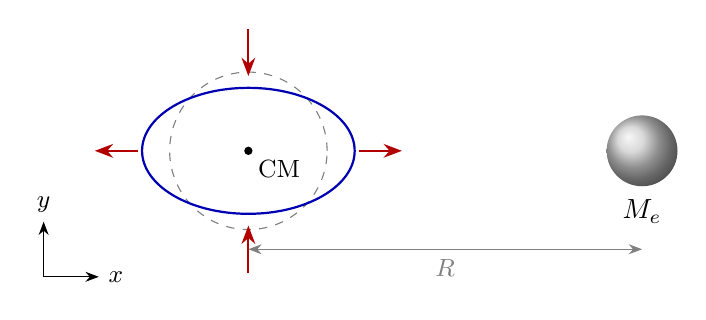
\begin{tikzpicture}[scale=1.0,>=Stealth]
  \draw[dashed,gray] (0,0) circle (1);
  \draw[thick,blue!70!black] (0,0) ellipse (1.35 and 0.8);
  \foreach \a in {0,180}{\draw[->,thick,red!70!black] (\a:1.4) -- (\a:1.95);}
  \foreach \a in {90,270}{\draw[->,thick,red!70!black] (\a:1.55) -- (\a:0.95);}
  \fill (0,0) circle (1.5pt);
  \node[below right,font=\small] at (0,0) {CM};
  \shade[ball color=gray!40] (5,0) circle (0.45);
  \node[below] at (5,-0.5) {$M_e$};
  \draw[->] (-2.6,-1.6) -- (-1.9,-1.6) node[right,font=\small] {$x$};
  \draw[->] (-2.6,-1.6) -- (-2.6,-0.9) node[above,font=\small] {$y$};
  \draw[gray,<->] (0,-1.25) -- (5,-1.25) node[midway,below,font=\small] {$R$};
\end{tikzpicture}
\end{center}
Since the tidal acceleration is $\propto GM_e r/R^3$, it falls off as $1/R^3$, whereas the gravitational acceleration itself falls off as $1/R^2$: this is why the Moon produces larger tides on the Earth than the Sun.
\end{carroll}
\end{points}

\chapter{The Equivalence Principle}

\section{Gravitational mass and inertial mass.}

\begin{points}
\item In Newtonian mechanics mass plays a fundamental role, since, through Newton's second law, it determines the acceleration that a body undergoes when it is subjected to a force,
\[
  \vec F=m\vec a .
\]
This parameter is called the inertial mass of the body.

\item On the other hand, the law of universal gravitation states that the gravitational force between two bodies is proportional to their mass.

\item From a conceptual point of view, the mass appearing in the law of universal gravitation is completely different from the previous one. In Newton's law it is a ``resistance'' of the particle to changing its velocity, whereas in gravitation it corresponds to the value of the gravitational ``charge'' of the particle, i.e.\ the property of the object that generates, and is affected by, the gravitational interaction.

\item Given the conceptual difference between the two, it is useful to distinguish them and to call \emph{gravitational mass} the mass term appearing in the law of universal gravitation.

\item From this point of view, we have two physical quantities that are a priori completely different and that, from an observational point of view, turn out to have the property of being proportional to each other, with a universal proportionality factor (which can therefore be chosen equal to one by a suitable choice of units).
\end{points}

\section{Galileo's equivalence principle.}

\begin{points}
\item This experimental fact is of such a fundamental nature that it can be raised to a principle of physics. This principle is known as ``Galileo's equivalence principle'' or also the ``weak equivalence principle''.

\item As with every physical principle, we must ask ourselves to what extent it has been tested experimentally.

\item Galileo Galilei (1564--1642) discovered that bodies fall at a rate independent of their mass. The usual way of describing these experiments is through the famous (and very probably apocryphal) experiment of Galileo dropping objects of different composition and density from the top of the Leaning Tower of Pisa to check that they all take the same amount of time to reach the ground.

\item The experiment that Galileo did perform consisted in letting two heavy objects roll down an inclined plane with a small angle of inclination, so that the fall time was long and the motion of objects of different compositions and sizes could thus be compared.

\item This experiment, together with improved versions by Huygens (1629--1695), allowed Newton to conclude that the force of gravity is proportional to the (inertial) mass of the object that falls. By Newton's third law one can conclude that the gravitational force is also proportional to the (inertial) mass of the object that creates the force.

\item However, Newton was fully aware that this hypothesis could be only approximate and that, therefore, the inertial mass of the second law could be different from the gravitational mass.

\item Distinguishing between the two by means of the symbols $m_i$ and $m_g$ respectively, and calling $\vec g$ the gravitational field generated by any (gravitational) mass distribution, the acceleration of a point particle with masses $m_i$ and $m_g$ is given by
\[
  \vec a=\frac{m_g}{m_i}\vec g .
\]
The experimental hypothesis to be tested is whether the ratio $m_g/m_i$ can be different for different bodies.

\item Under these conditions, a pendulum of length $\ell$ performing small oscillations has a period
\[
  T=2\pi\sqrt{\frac{m_i\ell}{m_gg}} .
\]

\item By taking pendulums of equal length and different compositions, one can compare the periods and see to what extent they coincide.

\item Newton carried out this kind of experiment and observed no differences in the periods of the pendulums.

\item These experiments were improved by Bessel in 1830, also with negative results for the difference in the periods.

\item However, the measurements of the periods of pendulums are not precise enough (essentially because of the damping of the pendulum), so the equality between inertial and gravitational mass could be established with a precision of at most $10^{-3}$.

\item In 1889 Loránd von Eötvös, of Budapest, devised a much more precise method to test experimentally the equality between inertial and gravitational mass. His method made it possible to conclude that the ratio $\frac{m_i}{m_g}$ for two different substances does not differ by more than one part in $10^9$, which is a really very high precision.

\item The method consists in using the rotation of the Earth and the centrifugal acceleration that it generates in a reference frame attached to the laboratory.

\item The experimental set-up is the following: two equal masses joined by a rod 40\,cm long are suspended.

\item The following external forces act on the rod:

(i) The force of gravity $\vec F_g=m_g\vec g$ on each of the particles $A$ and $B$.

(ii) The centrifugal force on each of the particles. Being an inertial force, it is proportional to the inertial mass of the particles,
\[
  \vec F_C=-m_i\vec\omega\times(\vec\omega\times\vec r),
\]
where $\vec\omega$ is the angular velocity of rotation of the Earth and $\vec r$ is the position vector of the particle with respect to the centre of the Earth. Writing $\vec r=\vec R_C+\vec r\,'$, where $\vec R_C$ is the position vector of the suspension point $C$ with respect to the centre of the Earth and $\vec r\,'$ the position of the particle relative to the point $C$, we can approximate the centrifugal force by
\[
  \vec F_C=-m_i\vec\omega\times\left(\vec\omega\times\vec R_C\right).
\]

(iii) The force exerted by the suspension fibre of the rod, which is directed along the fibre itself.

(iv) In addition, because of the torsion of the fibre, the latter exerts a torque on the rod, directed along the fibre itself.

\item We place ourselves at the equilibrium position of the system, in which the rod is horizontal. We call $\vec e_1$ the unit vector at $C$ along the fibre, and $\vec e_2$ the unit vector at $C$ pointing from particle $A$ towards $B$.

\item We define $\vec g_C:=\vec\omega\times\left(\vec\omega\times\vec R_C\right)$, so that the centrifugal force on each particle is $\vec F_C=-m_i\vec g_C$.

\item We call $m_i^A$ and $m_i^B$ the inertial masses of the particles $A$ and $B$, and $m_g^A$, $m_g^B$ their gravitational masses.

\item The equilibrium condition for the forces and for the torques imposes the conditions
\begin{gather*}
  T\vec e_1+(m_g^A+m_g^B)\vec g-(m_i^A+m_i^B)\vec g_C=0,\\
  M\vec e_1+l_B\vec e_2\times\left(m_g^B\vec g-m_i^B\vec g_C\right)-l_A\vec e_2\times\left(m_g^A\vec g-m_i^A\vec g_C\right)=0
\end{gather*}
where $l_A$ is the length between the point $C$ and the point $A$, and similarly for $l_B$.

\item We solve the first equation to obtain $\vec g$:
\[
  \vec g=\frac{-T}{m_g^A+m_g^B}\vec e_1+\frac{m_i^A+m_i^B}{m_g^A+m_g^B}\vec g_C
\]
and substitute it into the torque-balance equation. Using
\begin{align*}
  m_g^B\vec g-m_i^B\vec g_C&=\frac{-Tm_g^B}{m_g^A+m_g^B}\vec e_1+\frac{m_g^Am_g^B}{m_g^A+m_g^B}\left(\frac{m_i^A}{m_g^A}-\frac{m_i^B}{m_g^B}\right)\vec g_C,\\
  m_g^A\vec g-m_i^A\vec g_C&=\frac{-Tm_g^A}{m_g^A+m_g^B}\vec e_1-\frac{m_g^Am_g^B}{m_g^A+m_g^B}\left(\frac{m_i^A}{m_g^A}-\frac{m_i^B}{m_g^B}\right)\vec g_C,
\end{align*}
we obtain
\[
  M\vec e_1+\frac{T}{m_g^A+m_g^B}\left(l_Bm_g^B-l_Am_g^A\right)\vec e_3+(l_A+l_B)\frac{m_g^Am_g^B}{m_g^A+m_g^B}\left(\frac{m_i^A}{m_g^A}-\frac{m_i^B}{m_g^B}\right)\vec e_2\times\vec g_C=0
\]

\item We conclude that the torque exerted by the fibre must be proportional to the quantity
\[
  \left(\frac{m_i^A}{m_g^A}-\frac{m_i^B}{m_g^B}\right).
\]
More precisely,
\[
  M=\mu_g\left(\frac{m_i^A}{m_g^A}-\frac{m_i^B}{m_g^B}\right)\vec e_1\cdot\left(\vec g_C\times\vec L\right)
\]
where $\vec L$ is the position vector of the mass $B$ with respect to $A$, and $\mu_g$ is the (gravitational) reduced mass of the system.

\item By measuring the deflection angle of the rod for different masses, we can determine $\left(\frac{m_i^A}{m_g^A}-\frac{m_i^B}{m_g^B}\right)$.

\item Eötvös's original experiment of 1889 was improved by Eötvös, Pekár and Fekete in 1922. The precision achieved was
\[
  \left|\frac{m_i-m_g}{m_g}\right|\leq3\cdot10^{-9}.
\]
The experiment was repeated by Dicke, Krotkov and Roll in 1964, using the orbital motion of the Earth around the Sun, instead of the rotation of the Earth, as the source of the field of inertial forces. They obtained
\[
  \left|\frac{m_i-m_g}{m_g}\right|\leq1.5\cdot10^{-11}.
\]
More recent measurements have provided the following bounds:
\begin{align*}
  &\text{Adelberger \emph{et al} (1990)}, && \frac{|\Delta m|}{m}=\left\{\begin{array}{ll}(0.2\pm1.0)\cdot10^{-11}&\quad\text{Cu / Be}\\(0.5\pm1.3)\cdot10^{-11}&\quad\text{Al / Be}\end{array}\right.\\
  &\text{Baesler \emph{et al} (1999)}, && \frac{|\Delta m|}{m}\leq5\cdot10^{-13}
\end{align*}

There are several space missions under way or being designed to test the weak equivalence principle with higher precision. In April 2016 the MicroSCOPE satellite was launched with the aim of establishing a bound of $10^{-15}$. In December 2017 the first results of this mission were published, which indeed confirm the bound of $10^{-15}$ on the validity of the weak equivalence principle. The launch of a joint NASA/ESA satellite called STEP (Satellite Test of the Equivalence Principle) is also planned (with no specific date), with the mission of measuring $\Delta m/m$ with a precision of $10^{-18}$.
\end{points}

\section{Gravitational forces and inertial forces.}

\begin{points}
\item Galileo's equivalence principle thus has a very good experimental basis.

\item What consequences can we draw from this principle?

\item If we consider a Cartesian reference frame $S$ that moves (without rotating) with acceleration $\vec a_0(t)$ with respect to an inertial one, and we want to write Newton's laws in the frame $S'$, we must include a non-inertial force $\vec F_I=-m_i\vec a$, so that Newton's law in $S$ is
\[
  m_i\vec a=\vec F-m_i\vec a_0
\]
where $\vec F$ is the set of applied forces. On the other hand, the motion of a particle with respect to an inertial reference frame, on which a uniform gravitational force acts in addition to the applied forces $\vec F$, is given by Newton's law
\[
  m_i\vec a=\vec F+m_g\vec g .
\]
The two situations are completely indistinguishable from the dynamical point of view provided that $\vec g=-\vec a_0$.

\item We conclude that in Newtonian mechanics the laws of dynamics are equivalent for a reference frame with constant acceleration (with respect to an inertial one) and for an inertial reference frame with a constant and uniform gravitational field.

\item Let us recall Galileo's principle of relativity: \emph{It is impossible to determine by mechanical processes whether a reference frame is at rest or in uniform rectilinear motion}. In other words, the laws of mechanics are equivalent in a given inertial reference frame and in any other reference frame moving with constant velocity with respect to the former.

\item The weak equivalence principle seems to indicate that accelerated reference frames and inertial reference frames with gravitational fields could be indistinguishable by means of mechanical processes.

\item However, the previous equivalence relied heavily on the fact that $\vec g$ is uniform.

\item If we consider an arbitrary gravitational field $\vec g(\vec x,t)$, it will not be possible to put a Cartesian reference frame $S$ in a state of motion such that the inertial force corresponds to $m\vec g$.

\item However, we can consider a reference frame $S'$ that does not rotate with respect to the previous one and whose origin $O'$ follows a free-fall trajectory in the field $\vec g(\vec x,t)$. If we consider a particle on which no force acts other than gravity, and which is located near $O'$ and initially moving with velocity $\vec v$ with respect to $O'$, we can ask ourselves what motion $S'$ will see.

\item The answer is that, as long as the particle does not move too far from the origin $O'$ (compared with the scales of inhomogeneity of $\vec g(\vec x,t)$), $O'$ will see the particle moving with constant velocity $\vec v$.

\item For example, if in a freely falling satellite we let go of a pen, it will move away from us with practically constant velocity. Although the gravitational field in which it is located is not uniform, on the scale of the satellite the variations of the field are very small and the effects of these inhomogeneities are negligible.

\item What we have achieved is to cancel the effect of the gravitational field by letting ourselves fall in it. If we had no information about the kind of frame we were in, we could argue that, since we observe that free particles do not accelerate, our reference frame is inertial and no external gravitational field acts.

\item Naturally, this cancellation of the gravitational field is only local, both in space and in time.

\item For example, let us consider an elevator in free fall in the gravitational field of the Earth. If we are inside it we will not notice any weight. We can ask ourselves what happens to two particles that we release from rest at the same height (inside the elevator). Since both particles move attracted by the Earth, their motion will be radial towards the centre of the Earth. Seen from the elevator, we will see that the two particles approach each other very slowly (and this attraction has nothing to do with their own mutual gravitational attraction, which we are neglecting completely). This is a tidal force, which corresponds to variations of the gravitational field.

\begin{carroll}[: why only locally]
In a sealed box accelerated by a rocket in empty space, free particles released from rest always ``fall'' along parallel straight lines, with the same acceleration. In a large box at rest (or freely falling) in the gravitational field of the Earth, they move instead towards the centre of the Earth, i.e.\ along \emph{converging} directions. By observing such relative motions an observer inside a sufficiently large box could distinguish a gravitational field from a uniform acceleration. This is why the equivalence between the two only holds in sufficiently small regions of space-time, where these inhomogeneities (tidal effects) cannot be detected.
\begin{center}
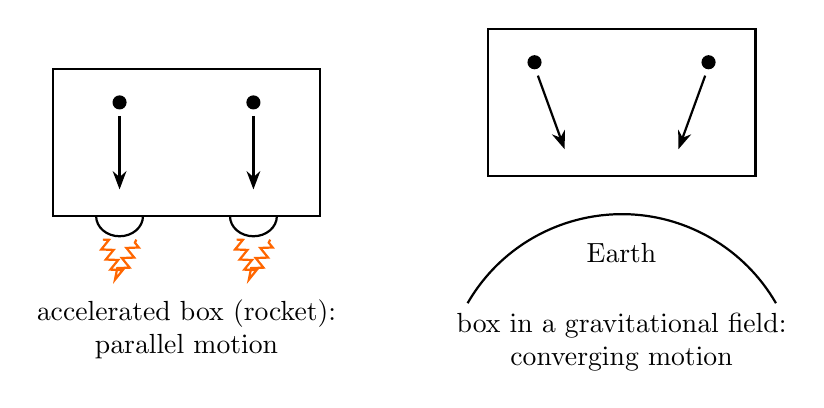
\begin{tikzpicture}[scale=0.85,>=Stealth]
  \begin{scope}
    \draw[thick] (0,0) rectangle (4,2.2);
    \foreach \x in {1,3}{\fill (\x,1.7) circle (3pt); \draw[->,thick] (\x,1.5) -- (\x,0.4);}
    \foreach \x in {1,3}{\draw[thick] (\x-0.35,0) arc (180:360:0.35 and 0.3);
      \draw[orange!80!red,thick,decorate,decoration={zigzag,amplitude=2pt,segment length=4pt}] (\x-0.25,-0.35) -- (\x,-0.9) -- (\x+0.25,-0.35);}
    \node[below,align=center] at (2,-1.1) {accelerated box (rocket):\\ parallel motion};
  \end{scope}
  \begin{scope}[shift={(6.5,0)}]
    \draw[thick] (0,0.6) rectangle (4,2.8);
    \fill (0.7,2.3) circle (3pt); \fill (3.3,2.3) circle (3pt);
    \draw[->,thick] (0.75,2.1) -- (1.15,1.0);
    \draw[->,thick] (3.25,2.1) -- (2.85,1.0);
    \draw[thick] (-0.3,-1.3) arc (150:30:2.66);
    \node at (2,-0.55) {Earth};
    \node[below,align=center] at (2,-1.3) {box in a gravitational field:\\ converging motion};
  \end{scope}
\end{tikzpicture}
\end{center}
\end{carroll}

\item We conclude that the reference frame is inertial (for mechanical processes) on scales on which tidal forces are negligible.
\end{points}

\section{Einstein's equivalence principle.}

\begin{points}
\item One of Einstein's great merits was to raise these mechanical properties, which are a consequence of Newton's laws and of Galileo's equivalence principle, to a principle of physics (and therefore conceptually prior to Newton's laws), and furthermore to extend it to all the laws of physics. This is a very important conceptual leap, which was not based on any previous experiment.
\end{points}

\textbf{Principle 1} (Einstein's equivalence principle)\textbf{.} \emph{All the laws of physics (except gravitation) are the same, on sufficiently local scales, in a freely falling reference frame in the presence of a gravitational field or in an inertial reference frame in the absence of gravity.}

An alternative version of this principle is:

\emph{The laws of physics (except gravitation) are the same, on sufficiently local scales, in an inertial reference frame with a gravitational field and in an accelerated reference frame.}

\begin{points}
\item This principle turned out to be the key for Einstein to be able to develop a theory of gravitation incorporating the essential principles of special relativity.

This process was not easy. Einstein published the equivalence principle in 1907 and it took him 8 years to develop his theory of gravity, which was named the theory of general relativity.

\item Part of the difficulty (but not all of it) was that Einstein had to learn the appropriate mathematics in which the new theory had to be formulated. In this task he had the help of a colleague and friend, the mathematician Marcel Grossmann.
\end{points}

\section{Space-time geometry and gravity.}

\begin{points}
\item Before entering the theory proper, we can draw some basic consequences of Einstein's equivalence principle.

\item Let us consider a ray of light moving in an inertial reference frame without gravitational fields. Its trajectory will be a straight line travelled at constant speed $c$.

\item Let us consider first a merry-go-round rotating with constant angular velocity about an axis parallel to the ray of light. This frame is non-inertial and the trajectory it observes for the ray of light is a helix. This is a curved trajectory. Since the ray moves very fast, under normal conditions we will not be able to observe this curvature. To see a substantial piece of the helix (and therefore notice the curvature of the trajectory), the frame must rotate at a sufficiently high speed. More precisely, $\omega D$ must be comparable with $c$, where $D$ is the distance between the trajectory of the light and the axis of the merry-go-round.

\item By the (Einstein) equivalence principle we conclude that a ray of light in the presence of a gravitational field follows a curved trajectory.

\item We can describe another example of the same phenomenon in the following way. Let us consider an elevator with a small slit on one side through which a ray of light enters. The elevator is in free fall in the gravitational field of the Earth. By the equivalence principle, the reference frame of the elevator is equivalent to an inertial one, so the ray of light must move in a straight line with respect to the elevator. For this to happen, the trajectory of the ray as seen from the Earth must bend downwards. We reach the same conclusion as before: the gravitational field bends the trajectories of light rays.

\item Let us consider again an inertial reference frame $S$ and another one $S'$ that rotates with respect to the former, and let us assume that there is no gravitational field (with respect to the frame $S$). We choose the $z$ and $z'$ axes along the rotation axis.

\item Let us take a circle centred at the origin (formed, for example, by a thin tube) and in the plane perpendicular to the $z$ axis. The inertial reference frame measures a length $\ell$ of the tube and a diameter $d$ of the circle, such that the ratio $\frac\ell d$ has the universal value
\[
  \frac\ell d=\pi .
\]

\item We can ask ourselves what the observer in the reference frame $S'$ measures. By symmetry, this observer must still see a circle (all its points must be at the same distance from the origin $O'$). To measure lengths, it must use rulers at rest in its own reference frame. The rulers used to measure the diameter of the circle move (with respect to the inertial frame $S$) in a direction perpendicular to the ruler, so that according to special relativity they have the same length both in $S$ and in $S'$. We conclude that $S'$ still measures $d$ as the diameter of the circle.

\item On the other hand, the rulers used to measure the perimeter of the circle move with longitudinal velocity $\frac{\omega d}{2}$, so that according to $S$ they have a length
\[
  L=L_0\sqrt{1-\frac{v^2}{c^2}}=L_0\sqrt{1-\frac{d^2\omega^2}{4c^2}},\qquad L_0=\text{proper length of the ruler}
\]
because of the length contraction of special relativity. Therefore, for them to cover the whole length of the circle, $S$ asserts that the number of rulers that must be placed is $n=\frac{\ell}{L_0\sqrt{1-\frac{d^2\omega^2}{4c^2}}}$. This is a natural number that counts objects, so $S'$ must count exactly the same number of rulers. Consequently, the perimeter of the circle according to $S'$ is
\[
  \ell'=nL_0=\frac{\ell}{\sqrt{1-\frac{d^2\omega^2}{4c^2}}} .
\]
The ratio between perimeter and diameter is
\[
  \frac{\ell'}{d'}=\frac\ell d\frac{1}{\sqrt{1-\frac{d^2\omega^2}{4c^2}}}=\frac{\pi}{\sqrt{1-\frac{d^2\omega^2}{4c^2}}}>\pi
\]
and we reach the conclusion that the geometry of space according to $S'$ cannot be Euclidean.

\item By the equivalence principle, the presence of gravitational fields also modifies the geometry of space, which can no longer be Euclidean.

\item A third important consequence of the equivalence principle is that the frequency of a photon changes along its trajectory in a gravitational field. This effect is known as the \textbf{gravitational Doppler effect}.

\item We can argue for it by means of the following \emph{Gedankenexperiment}, proposed by Einstein himself.

\item Let us consider a tower of height $h$ on the surface of the Earth, and let us suppose that we drop an object of mass $m$ from the top.

\item When the particle reaches the bottom it has kinetic energy, so that its total energy is greater than its rest energy.

\item Let us suppose that the particle is instantaneously transformed into a photon with the same energy and moving upwards (although this process violates the conservation of linear momentum, we can think that this conversion occurs just as the particle reaches the ground, so that the linear momentum is absorbed by the Earth, in the same way as in the elastic bounce of a ball against a wall).

\item Let us suppose that, when the photon reaches the top of the tower, the inverse process occurs and the photon turns into a material particle at rest (again, the difference in linear momentum can be absorbed by the tower and, ultimately, by the Earth).

\item If the photon did not change its frequency while climbing the tower, the final inertial mass $m'$ would be strictly greater than the initial one, $m'>m$, and we could build a perpetual motion machine of the first kind and violate the conservation of energy, which is one of the pillars of physics.

\item We conclude that the photon must decrease its frequency (energy) when it climbs in the gravitational field.

\item We can make an approximate calculation of how the frequency of the photon must change. The energy of the particle arriving at the bottom is
\[
  \frac{mc^2}{\sqrt{1-\frac{v^2}{c^2}}}=mc^2+\frac12mv^2+O\left(\frac{v^4}{c^4}\right).
\]

\item Using Newton's law, the speed at which it arrives at the bottom is $v=\sqrt{2gh}$, where $h$ is the height of the tower. Therefore $E_f=mc^2+mgh+O(v^4/c^4)$.

\item For energy to be conserved, the photon at the top must have an energy satisfying
\[
  \frac{E'_\gamma}{E^0_\gamma}=\frac{mc^2}{mc^2+mgh+O(4)}=1-\frac{hg}{c^2}+O(4)=\frac{\nu'}{\nu_0}
\]

\item Therefore, in its ascent the photon undergoes a Doppler effect (redshift) described by the following expression
\[
  \nu'=\nu_0\left(1-\frac{gh}{c^2}+O(4)\right).
\]

\item This is a measurable effect. In 1959 Pound and Rebka devised the following experiment (later improved by Pound and Snider in 1965). It consisted in measuring the change in frequency of a photon climbing a column 22.5 metres high (which corresponds to a relative frequency change of $\frac{gh}{c^2}=2.5\cdot10^{-15}$). The experiment was carried out at the Jefferson Laboratory at Harvard. The method used to measure the frequencies consisted in using the Mössbauer effect, i.e.\ the existence of resonances in the absorption and emission of gamma rays by the nuclei of the atoms of a solid. The result of the experiment was the confirmation of the gravitational Doppler effect with a precision of 1\%.

\begin{carroll}[: the gravitational redshift from accelerated boxes, and why space-time is curved]
\textit{(a) Accelerated boxes.} Consider two boxes, a distance $z$ apart, moving far away from any matter with the same constant acceleration $a$. At time $t_0$ the trailing box emits a photon of wavelength $\lambda_0$. The boxes keep a constant distance, so the photon reaches the leading box after $\Delta t=z/c$, during which the boxes have picked up an additional velocity $\Delta v=a\Delta t=az/c$. To first order in $\Delta v/c$, the photon reaching the leading box is therefore redshifted by the ordinary Doppler effect,
\[
  \frac{\Delta\lambda}{\lambda_0}=\frac{\Delta v}{c}=\frac{az}{c^2}.
\]
By the equivalence principle the same must happen in a tower of height $z$ on the surface of a planet, with $a\to g$, which reproduces the result above ($\nu'/\nu_0=1-gh/c^2$). For a non-uniform field one integrates along the path, $\frac{\Delta\lambda}{\lambda_0}=\frac{1}{c^2}\int\partial_z\Phi\,dz=\frac{\Delta\Phi}{c^2}$.
\begin{center}
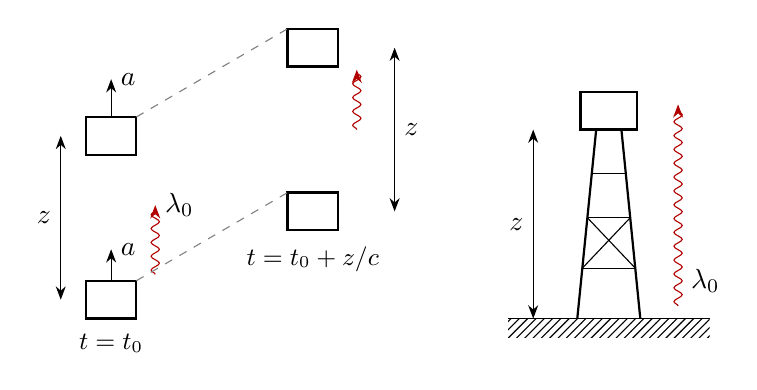
\begin{tikzpicture}[scale=0.8,>=Stealth]
  % accelerated boxes
  \draw[thick] (0,0) rectangle (0.8,0.6); \draw[thick] (0,2.6) rectangle (0.8,3.2);
  \draw[->] (0.4,3.2) -- (0.4,3.8) node[right] {$a$};
  \draw[->] (0.4,0.6) -- (0.4,1.1) node[right] {$a$};
  \draw[decorate,decoration={snake,amplitude=1.5pt,segment length=5pt},->,red!70!black] (1.1,0.7) -- (1.1,1.8) node[right,black] {$\lambda_0$};
  \draw[<->] (-0.4,0.3) -- (-0.4,2.9) node[midway,left] {$z$};
  \node[below] at (0.4,-0.1) {\small $t=t_0$};
  \begin{scope}[shift={(3.2,1.4)}]
    \draw[thick] (0,0) rectangle (0.8,0.6); \draw[thick] (0,2.6) rectangle (0.8,3.2);
    \draw[decorate,decoration={snake,amplitude=1.5pt,segment length=5pt},->,red!70!black] (1.1,1.6) -- (1.1,2.55);
    \draw[<->] (1.7,0.3) -- (1.7,2.9) node[midway,right] {$z$};
    \node[below] at (0.4,-0.1) {\small $t=t_0+z/c$};
  \end{scope}
  \draw[dashed,gray] (0.8,0.6) -- (3.2,2.0); \draw[dashed,gray] (0.8,3.2) -- (3.2,4.6);
  % tower
  \begin{scope}[shift={(7.5,0)}]
    \fill[pattern=north east lines] (-0.8,-0.3) rectangle (2.4,0);
    \draw (-0.8,0) -- (2.4,0);
    \draw[thick] (0.3,0) -- (0.6,3.0) -- (1.0,3.0) -- (1.3,0);
    \draw (0.38,0.8) -- (1.22,0.8) (0.46,1.6) -- (1.14,1.6) (0.53,2.3) -- (1.07,2.3);
    \draw (0.38,0.8) -- (1.14,1.6) (1.22,0.8) -- (0.46,1.6);
    \draw[thick] (0.35,3.0) rectangle (1.25,3.6);
    \draw[decorate,decoration={snake,amplitude=1.5pt,segment length=5pt},->,red!70!black] (1.9,0.2) -- (1.9,3.4);
    \node[right] at (1.95,0.6) {$\lambda_0$};
    \draw[<->] (-0.4,0) -- (-0.4,3.0) node[midway,left] {$z$};
  \end{scope}
\end{tikzpicture}
\end{center}

\textit{(b) Why space-time must be curved.} A physicist on the ground emits a beam of light from height $z_0$, received at the top of the tower at height $z_1$. The time between the emission of the beginning and of the end of one wavelength is $\Delta t_0=\lambda_0/c$, and the time between the reception of the beginning and of the end is $\Delta t_1=\lambda_1/c$. Since the gravitational field does not change with time, the paths in space-time followed by the leading and trailing edges of the wave must be precisely congruent (a time translation of each other, see the figure). In a flat space-time simple geometry would then tell us that $\Delta t_1=\Delta t_0$. But the gravitational redshift implies $\Delta t_1>\Delta t_0$ (``the clock at the top of the tower appears to run faster''). The fault lies with the ``simple geometry'': a better description is to admit that space-time is curved.
\begin{center}
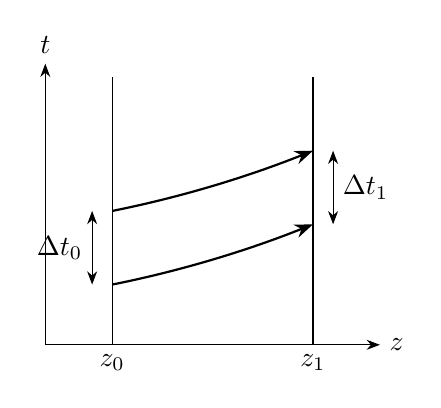
\begin{tikzpicture}[scale=0.85,>=Stealth]
  \draw[->] (0,0) -- (5,0) node[right] {$z$};
  \draw[->] (0,0) -- (0,4.2) node[above] {$t$};
  \draw (1,0) -- (1,4); \draw (4,0) -- (4,4);
  \node[below] at (1,0) {$z_0$}; \node[below] at (4,0) {$z_1$};
  \draw[thick,->] (1,0.9) .. controls (2,1.1) and (3,1.4) .. (4,1.8);
  \draw[thick,->] (1,2.0) .. controls (2,2.2) and (3,2.5) .. (4,2.9);
  \draw[<->] (0.7,0.9) -- (0.7,2.0) node[midway,left] {$\Delta t_0$};
  \draw[<->] (4.3,1.8) -- (4.3,2.9) node[midway,right] {$\Delta t_1$};
\end{tikzpicture}
\end{center}
\end{carroll}

\item We have already seen that the spatial geometry for an accelerated observer (and therefore also in the presence of a gravitational field) is no longer Euclidean. We also know that, because of special relativity, space and time form a four-dimensional entity called space-time. The space-time of special relativity is described by a metric called the Minkowski metric, which takes the form
\[
  ds^2=-c^2dt^2+dx^2+dy^2+dz^2
\]
where $t,x,y,z$ are the Cartesian time and space coordinates associated with an inertial reference frame.

\item This metric is used to measure space-time intervals between two events. In cylindrical coordinates $\{t,\rho,\phi,z\}$ the Minkowski metric takes the form
\[
  ds^2=-c^2dt^2+d\rho^2+\rho^2d\phi^2+dz^2 .
\]
If we now consider a reference frame rotating with constant velocity around the $z$ axis, a point that initially had coordinates $\{\rho',\phi',z'\}$ and that rotates with constant angular velocity follows the trajectory
\[
  \rho(t)=\rho',\qquad\phi(t)=\phi'+\omega t,\qquad z(t)=z' .
\]
The reference frame $S'$ can decide to coordinatise the events of space-time in such a way that all the points of the previous trajectories are identified by the values $\{\rho',\phi',z'\}$ and by the time $t$ of the clocks in $S$. Therefore the coordinate transformation between the two reference frames is
\[
  \left\{\begin{array}{l}t=t'\\ \rho=\rho'\\ \phi=\phi'+\omega t'\\ z=z'\end{array}\right.
\]

\item If we write the Minkowski metric in the new coordinates we obtain
\begin{align*}
  ds^2&=-c^2dt'^2+d\rho'^2+\rho'^2\left(d\phi'+\omega dt'\right)^2+dz'^2\\
  &=-c^2\left(1-\frac{\rho'^2\omega^2}{c^2}\right)dt'^2+2\omega\rho'^2d\phi'dt'+d\rho'^2+\rho'^2d\phi'^2+dz'^2
\end{align*}
which obviously has a form different from the Minkowski form in the coordinates of the inertial reference frame.

\item By Einstein's equivalence principle we conclude that the space-time geometry of a space-time containing a gravitational field is described by a metric different from the Minkowskian form $-c^2dt^2+dx^2+dy^2+dz^2$.

\item Therefore, we must be able to handle space-times with arbitrary Lorentzian metrics and to derive geometric consequences from them. For this, it is necessary to develop the fundamental tools of differential geometry.
\end{points}

\chapter{Introduction to differential geometry}

\section{Differentiable manifold.}

\begin{points}
\item The basic object of differential geometry is the \textbf{differentiable manifold}.

\item Intuitively, a differentiable manifold is a space of points that, locally (i.e.\ in some neighbourhood of each of its points), looks the same as a domain of $\R^n$.

\item The idea is that we can use local coordinates to describe sufficiently small regions of the manifold. This allows us to use all the tools of differential calculus in $\R^n$ without having to restrict ourselves to the space $\R^n$.

\item In fact, from a global point of view a differentiable manifold is, in general, completely different from $\R^n$.

\item Each of the coordinate systems that we can use to coordinatise the neighbourhood of some point is called a \textbf{local chart}. The set of all the local charts is called an \textbf{atlas}.

\item A fundamental property of differentiable manifolds is that all local charts are equally valid for drawing conclusions. This does not mean that in some charts the calculations cannot be simpler, but in principle all of them are allowed. There are no a priori privileged coordinates (as long as the chart belongs to the atlas of the manifold).

\item The simplest example of a differentiable manifold is $\R^n$ itself, in which we can use a single local chart (Cartesian coordinates) to describe all the points. However, we can also use many other charts. For example, spherical coordinates, which cover all the points except a line, cylindrical coordinates (which also cover all the points except a line), or many other coordinate systems. In general, each of them will be able to coordinatise a specific region of $\R^n$.

\item A differentiable manifold that is no longer globally $\R^2$ is the two-dimensional sphere. In this case we need at least two local charts to describe all the points of the manifold. In other words, if we want to represent the points of the terrestrial globe by a pair of numbers, we need to divide the sphere into at least two regions (which must necessarily intersect) and to use coordinates in each of them. For example, if we decide to use longitude and latitude as coordinates, we can cover the whole sphere except the North and South poles, with latitude $\theta=\pm\pi/2$, and the meridian corresponding to the values $\phi=\pi$ and $\phi=-\pi$. On this meridian the longitude coordinate stops varying continuously, so it must be excluded from the domain of the chart.

\item Naturally, there are many other local charts that allow us to describe regions of a two-dimensional sphere, for example the stereographic projection, or the Mercator projection, among many others.

\item The names local chart and atlas come from the historical need (fundamentally to allow navigation) to coordinatise regions of the terrestrial globe in order to describe them by means of (two-dimensional) sheets of paper.

\item More formally, to define a differentiable manifold we need to introduce the concept of topological space.

\item A set $\mathcal T$ is a topological space if a collection of subsets of $\mathcal T$ has been selected, which will be called the open sets of $\mathcal T$, with the following three properties:

(i) Both the empty set $\emptyset$ and the whole set $\mathcal T$ are open.

(ii) If $V_1$ and $V_2$ are open sets of $\mathcal T$, then $V_1\cap V_2$ is also open.

(iii) If $\{V_a\}$ is any collection of open sets of $\mathcal T$, then the union of all of them is also an open set of $\mathcal T$.

\item A topological space $\mathcal T$ is \textbf{connected} if there is no open set $V$ different from $\emptyset$ and from $\mathcal T$ itself such that $\mathcal T\setminus V$ is also open. In other words, we cannot decompose the whole space into two disjoint, non-empty open sets.

\item A differentiable manifold $M$ is a connected topological space together with an atlas (i.e.\ a collection of local charts) satisfying some compatibility properties. We define these concepts below.

\item A \textbf{local chart} is a pair $(U_a,\varphi_a)$, where each $U_a$ is an open set of $M$ and each
\[
  \varphi_a:U_a\longrightarrow\varphi_a(U_a)\subset\R^n
\]
is a continuous, invertible map with continuous inverse. These conditions imply in particular that the image $\varphi_a(U_a)$ is necessarily an open set of $\R^n$. An atlas is a collection of local charts with the condition that $M=\bigcup_aU_a$. The index $a$ takes values in a set on which we impose no restriction.

\item An atlas defines a structure of differentiable manifold of class $C^m$ on $M$, $m\in\mathbb N$, if for each pair of charts in the atlas, i.e.\ for each $a$ and $b$, the map
\[
  \varphi_a\circ\varphi_b^{-1}:\varphi_b(U_a\cap U_b)\longrightarrow\varphi_a(U_a\cap U_b)
\]
is of class $C^m$, or, in other words, it can be differentiated $m$ times with continuity.

\item If an atlas is $C^m$ for every $m$, the atlas is called $C^\infty$. In what follows we shall assume for simplicity that all differentiable manifolds are $C^\infty$.

\item The number $n$ is called the \textbf{dimension of the manifold}.

\item The map $\varphi_a\circ\varphi_b^{-1}$ is called the \textbf{transition function} or, more commonly, \textbf{change of coordinates}.

\item If we use $x^\alpha$ ($\alpha=1,\cdots,n$) to denote the Cartesian coordinates of $\R^n$, the map $\varphi_a\circ\varphi_b^{-1}$, which is a function from an open set of $\R^n$ to another open set of $\R^n$, will take the form of $n$ real functions of $n$ real variables, which we will denote by
\[
  y^\beta(x^\alpha)\qquad\alpha,\beta=1,\cdots,n
\]
or by
\[
  x^{\alpha'}(x^\alpha)\qquad\alpha,\alpha'=1,\cdots,n .
\]

\item In the second notation the coordinates are distinguished by their indices. This notation is especially convenient when carrying out calculations.
\end{points}

\begin{carroll}[: charts, transition functions and the sphere]
A chart $\varphi_a$ maps an open set $U_a\subset M$ one-to-one onto an open set of $\R^n$, where ordinary calculus is available. Where two charts overlap, the transition function $\varphi_a\circ\varphi_b^{-1}$ relates the two sets of coordinates of the same points; requiring it to be $C^\infty$ is what makes ``differentiable'' a chart-independent notion.
\begin{center}
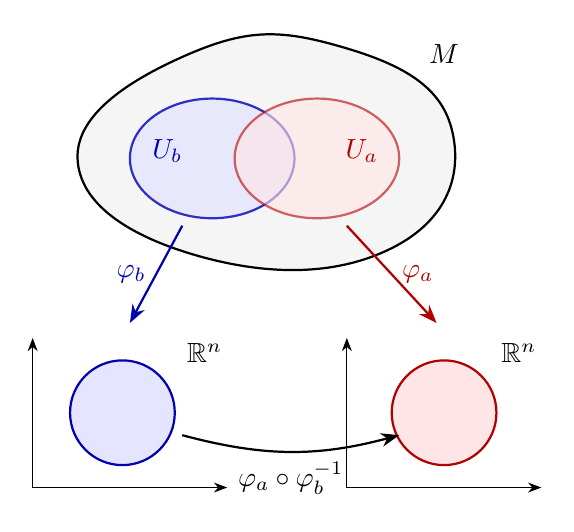
\begin{tikzpicture}[scale=0.95,>=Stealth]
  \draw[thick,fill=gray!8] plot[smooth cycle,tension=0.8] coordinates {(0,0.2) (1.5,1.6) (3.5,1.7) (5,0.6) (4.2,-1.0) (1.6,-1.1)};
  \node at (4.9,1.6) {$M$};
  \draw[thick,blue!70!black,fill=blue!10,opacity=0.8] (1.8,0.2) ellipse (1.1 and 0.8);
  \draw[thick,red!70!black,fill=red!10,opacity=0.6] (3.2,0.2) ellipse (1.1 and 0.8);
  \node[blue!70!black] at (1.2,0.3) {$U_b$};
  \node[red!70!black] at (3.8,0.3) {$U_a$};
  % R^n images
  \begin{scope}[shift={(-0.6,-4.2)}]
    \draw[->] (0,0) -- (2.6,0); \draw[->] (0,0) -- (0,2.0); \node at (2.3,1.8) {$\R^n$};
    \draw[thick,blue!70!black,fill=blue!10] (1.2,1.0) circle (0.7);
  \end{scope}
  \begin{scope}[shift={(3.6,-4.2)}]
    \draw[->] (0,0) -- (2.6,0); \draw[->] (0,0) -- (0,2.0); \node at (2.3,1.8) {$\R^n$};
    \draw[thick,red!70!black,fill=red!10] (1.3,1.0) circle (0.7);
  \end{scope}
  \draw[->,thick,blue!70!black] (1.4,-0.7) -- (0.7,-2.0) node[midway,left] {$\varphi_b$};
  \draw[->,thick,red!70!black] (3.6,-0.7) -- (4.8,-2.0) node[midway,right] {$\varphi_a$};
  \draw[->,thick] (1.4,-3.5) to[bend right=15] node[midway,below] {$\varphi_a\circ\varphi_b^{-1}$} (4.3,-3.5);
\end{tikzpicture}
\end{center}
For the two-dimensional sphere $S^2$ one can use, for example, two stereographic projections, from the North and from the South pole; each one covers the whole sphere except the pole from which it projects, and together they form an atlas. No single chart can cover $S^2$: a sphere is not homeomorphic to an open subset of $\R^2$.
\end{carroll}


\section{Vectors, 1-forms and tensors.}

\begin{points}
\item Given a differentiable manifold, we can define \textbf{differentiable curves}. These are maps
\[
  \gamma:(s,t)\subset\R\longrightarrow M
\]
which, expressed in local coordinates, give rise to a differentiable function of $(s,t)$ into $\R^n$. More precisely, for each $a$, the map $\varphi_a\circ\gamma:\gamma^{-1}(U_a)\subset(s,t)\longrightarrow\R^n$ must be a differentiable function.

\item Unless stated otherwise, by \emph{curve} we mean a \emph{differentiable curve}.

\item We can define tangent vectors at a point $p\in M$ by means of equivalence classes of curves ``that point in the same direction at $p$''.

\item To give a more direct definition we use the concept of directional derivative acting on scalar fields.

\item A scalar field is a differentiable map $f:M\longrightarrow\R$. A map is differentiable if its expression in each local chart gives rise to a function of a real variable that is $C^\infty$. More precisely, the expression of $f$ in a local chart is $f\circ\varphi_a^{-1}$. The domain of this map is the open set $\varphi_a(U_a)\subset\R^n$. We therefore have a real function of $n$ real variables, for which the notion of derivative makes sense, so we can impose the condition that this function be $C^\infty$.

\item If we express a function $f:M\longrightarrow\R$ in a set of local charts covering the manifold, and the resulting functions are $C^\infty$, the differentiability of $f$ is guaranteed. That is, it is not necessary to check the differentiability in the rest of the charts of the atlas.

\item If we are only interested in establishing the differentiability of $f$ in a neighbourhood of a point $p$, it is enough to check the differentiability in one local chart containing $p$. Differentiability in any other local chart containing $p$ is then automatically satisfied.

\item The local chart $(U_a,\varphi_a)$ will be denoted simply by $x^\alpha$, and the function $f\circ\varphi_a^{-1}$ by $f(x^\alpha)$.

\item We define a vector $V|_p$ at $p$ as an object that is able to act on scalar fields and to provide a numerical value, which we denote by $V(f)|_p\in\R$, and that satisfies the following conditions:

(ii) linearity: $V(f+g)|_p=V(f)|_p+V(g)|_p$, \quad $V(cf)|_p=cV(f)|_p$, for $c\in\R$.

(i) Leibniz rule: $V(fg)|_p=f(p)V(g)|_p+g(p)V(f)|_p$

\item Given a (differentiable) curve $\gamma:(s,t)\to M$, which we denote by $\gamma(\sigma)$, and a point $p=\gamma(\sigma_0)$, we can define a vector at $p$ called the \textbf{tangent vector to the curve at} $p$, which we denote by $\dot\gamma|_p$, by means of the expression
\[
  \dot\gamma|_p(f)=\left.\frac{d f(\gamma(\sigma))}{d\sigma}\right|_{\sigma_0}.
\]

\item Note that $f\circ\gamma:(s,t)\to\R$ is a real function of a real variable, so that the notion of derivative makes sense. It is immediate to check that this operation is a vector (in the sense that it satisfies the properties of linearity and the Leibniz rule).

\item Two curves defining the same vector at a point $p$ are called \textbf{tangent} at $p$.

\item On the other hand, given a vector $V|_p$ at $p$ there always exists a curve $\gamma(\sigma)$ passing through $p$ that has $V|_p$ as its tangent vector.

\item We define the sum of vectors and the product by scalars $a_1,a_2\in\R$ by
\[
  \left(a_1V_1+a_2V_2\right)(f)|_p:=a_1V_1(f)|_p+a_2V_2(f)|_p .
\]

\item The set of vectors at $p\in M$ forms a vector space, which we denote by $T_pM$ and call the \textbf{tangent space} to the manifold at the point $p$.

\item Given a local chart (which we will also call a coordinate system) $\{x^\alpha\}$ whose domain contains the point $p$, we can define a set of $n$ vectors $\left.\frac{\partial}{\partial x^\alpha}\right|_p$ by means of the expression
\[
  \left.\frac{\partial}{\partial x^\alpha}\right|_p(f):=\left.\frac{\partial f(x^\beta)}{\partial x^\alpha}\right|_{x(p)} .
\]

\item We will also denote the vector $\left.\frac{\partial}{\partial x^\alpha}\right|_p$ by $\partial_{x^\alpha}|_p$ or by $\partial_\alpha|_p$.

\item One can prove that (i) $\partial_\alpha|_p$ is a vector (i.e.\ it satisfies the properties of linearity and the Leibniz rule), (ii) the set of $n$ vectors $\{\partial_\alpha|_p\}$ ($\alpha=1,\cdots,n$) is linearly independent, and (iii) any vector $V_p\in T_pM$ can be expressed as a linear combination of them, i.e.\ there exist $n$ constants $V^\alpha|_p\in\R$, $\alpha=1,\cdots,n$, such that
\[
  V_p=V^\alpha|_p\partial_{x^\alpha}|_p .
\]

\item These properties show that the dimension of the vector space $T_pM$ is $n$, the same as the dimension of the manifold.

\item The vector $\partial_{x^1}$ is the tangent vector to the curve $\{x^1=\sigma,x^2=x_0^2,\cdots,x^n=x_0^n\}$. This curve is called the \textbf{coordinate line} $x^1$. Analogously, the coordinate line $x^\alpha$ is the curve defined by the rest of the coordinates $x^{\beta\neq\alpha}=\text{const}$ and $x^\alpha=\sigma$.

\item We can imagine the set of coordinate lines forming a mesh in the open set $U$ of the manifold where this coordinate system is defined. The basis tangent vectors $\partial_{x^\alpha}|_p$ are the $n$ independent directions that point along each of the directions of the mesh.

\item The coefficients $V^\alpha|_p$ are called the \textbf{components} of the vector $V|_p$ in the coordinate system $\{x^\alpha\}$.

\item The basis $e_\alpha|_p:=\partial_{x^\alpha}|_p$ is called the \textbf{natural basis} associated with the coordinates $\{x^\alpha\}$, or simply the coordinate basis.

\item Suppose we have two different coordinate systems in a neighbourhood of a point $p$ (i.e.\ both local charts contain $p$ in their domain). The coordinate change functions $x^{\alpha'}(x^\alpha)$ are $n$ functions of $n$ variables, invertible and $C^\infty$.

\item We therefore have two bases of vectors $\partial_{x^\alpha}|_p$ and $\partial_{x^{\alpha'}}|_p$, so there must exist a change-of-basis matrix.

\item Using the fact that vectors are derivations and using the chain rule we obtain, for any scalar function $f:M\to\R$,
\[
  \left.\frac{\partial f(x)}{\partial x^\alpha}\right|_{x(p)}=\left.\frac{\partial f(x')}{\partial x^{\alpha'}}\right|_{x'(p)}\left.\frac{\partial x^{\alpha'}}{\partial x^\alpha}\right|_{x(p)}
\]

\item Since this property holds for every $f$, we have the following relation between the vectors
\[
  \partial_{x^\alpha}|_p=\left.\frac{\partial x^{\alpha'}}{\partial x^\alpha}\right|_{x(p)}\partial_{x^{\alpha'}}\big|_p .
\]

\item The change-of-basis matrix between the coordinate bases is the Jacobian of the coordinate change $x^{\alpha'}(x^\alpha)$ evaluated at the point $p$.

\item Like any other vector space, $T_pM$ has an associated dual space $T^\star_pM$, which is called the cotangent space to the manifold at $p$. The elements of $T^\star_pM$ are called 1-forms or covectors.

\item To determine a basis of 1-forms, we first define the differential of a scalar function at a point $p$. Let $f:M\to\R$ be a scalar function. We want to define the differential of $f$ at $p\in M$ in such a way that it is a covector in $T^\star_pM$. Therefore, we must determine how it acts on vectors of $T_pM$. We define
\[
  df|_p(V|_p):=V|_p(f).
\]

\item Note that $f$ only needs to be defined in a neighbourhood of $p$ for its differential to exist.

\item Given a coordinate system $\{x^\alpha\}$ on a domain $U$ containing $p$, each of the maps $x^\alpha:U\to\R$ is a scalar function, and therefore we can define its differential at $p$.

\item The set of 1-forms $\{dx^\alpha|_p\}$ constitutes the dual basis of the coordinate basis $\{\partial_\alpha|_p\}$. Indeed
\[
  dx^\alpha|_p(\partial_{x^\beta}|_p)=\partial_{x^\beta}|_p(x^\alpha)=\left.\frac{\partial x^\alpha}{\partial x^\beta}\right|_{x(p)}=\delta^\alpha_\beta .
\]

\item The basis $\{dx^\alpha|_p\}$ associated with a coordinate system $\{x^\alpha\}$ is called the natural cobasis at $p$. Since they form a basis, any 1-form $\omega|_p\in T^\star_pM$ can be decomposed as
\[
  \omega|_p=\omega_\alpha|_pdx^\alpha|_p .
\]

\item The coefficients $\omega_\alpha|_p$ are called the components of the 1-form $\omega$ in the cobasis $\{dx^\alpha|_p\}$.

\item Given a coordinate change $x^{\alpha'}=x^{\alpha'}(x^\beta)$, we can relate the two corresponding natural cobases. We have
\[
  dx^{\alpha'}|_p\left(\partial_{x^\beta}|_p\right)=dx^{\alpha'}|_p\left(\left.\frac{\partial x^{\beta'}}{\partial x^\beta}\right|_{x(p)}\partial_{x^{\beta'}}|_p\right)=\left.\frac{\partial x^{\alpha'}}{\partial x^\beta}\right|_{x(p)}
  \quad\Longrightarrow\quad dx^{\alpha'}|_p=\left.\frac{\partial x^{\alpha'}}{\partial x^\alpha}\right|_{x(p)}dx^\alpha|_p .
\]

\item Once we have $T_pM$ and $T^\star_pM$, we can define the vector space of tensors at a point.

\item A tensor $r$ times covariant and $s$ times contravariant (where $r,s\in\mathbb N$) at $p\in M$ is a multilinear map
\[
  T:\underbrace{T^\star_pM\times\cdots\times T^\star_pM}_{s\text{ times}}\times\underbrace{T_pM\times\cdots\times T_pM}_{r\text{ times}}\longrightarrow\R
\]

\item The set of tensors $r$ times covariant and $s$ times contravariant is denoted by
\[
  \underbrace{T_pM\otimes\cdots\otimes T_pM}_{s\text{ times}}\otimes\underbrace{T^\star_pM\otimes\cdots\otimes T^\star_pM}_{r\text{ times}}:=(T_pM)^s_r
\]

\item If $\{e_\alpha|_p\}$ is a basis of $T_pM$ (for example a natural basis, although it can be any other) and $\theta^\alpha|_p$ is its dual basis (i.e.\ the one satisfying $\theta^\alpha|_p(e_\beta|_p)=\delta^\alpha_\beta$), we can define a set of $n^{r+s}$ tensors $r$ times covariant and $s$ times contravariant, $e_{\alpha_1}\otimes\cdots\otimes e_{\alpha_s}\otimes\theta^{\beta_1}\otimes\cdots\otimes\theta^{\beta_r})|_p$, by means of
\[
  e_{\alpha_1}\otimes\cdots\otimes e_{\alpha_s}\otimes\theta^{\beta_1}\otimes\cdots\otimes\theta^{\beta_r}|_p(\theta^{\mu_1}|_p,\cdots,\theta^{\mu_s}|_p,e_{\nu_1}|_p,\cdots,e_{\nu_r}|_p)=\delta^{\mu_1}_{\alpha_1}\cdots\delta^{\mu_s}_{\alpha_s}\cdot\delta^{\beta_1}_{\nu_1}\cdots\delta^{\beta_r}_{\nu_r}.
\]

\item It is easy to prove that this set of tensors is linearly independent and that any tensor $r$ times covariant and $s$ times contravariant can be expressed as a linear combination of them. Therefore, the set of $n^{r+s}$ tensors $e_{\alpha_1}\otimes\cdots\otimes e_{\alpha_s}\otimes\theta^{\beta_1}\otimes\cdots\otimes\theta^{\beta_r}|_p$ forms a basis of $(T_pM)^s_r$. This vector space therefore has dimension $n^{r+s}$.

\item The decomposition of any tensor $\mathcal T\in(T_pM)^s_r$ in this basis introduces a set of $n^{r+s}$ coefficients, called the \textbf{components} of the tensor. These coefficients are defined by the decomposition
\[
  \mathcal T=\left.\mathcal T^{\alpha_1\cdots\alpha_s}_{\beta_1\cdots\beta_r}\right|_pe_{\alpha_1}\otimes\cdots\otimes e_{\alpha_s}\otimes\theta^{\beta_1}\otimes\cdots\otimes\theta^{\beta_r}|_p .
\]

\item In a completely equivalent way we can write
\[
  \left.\mathcal T^{\alpha_1\cdots\alpha_s}_{\beta_1\cdots\beta_r}\right|_p=\mathcal T(\theta^{\alpha_1},\cdots,\theta^{\alpha_s},e_{\beta_1}\cdots e_{\beta_r}).
\]

\item If we consider a different basis $\{e_{\alpha'}|_p\}$ and its corresponding dual basis $\{\theta^{\alpha'}|_p\}$ (for example the natural bases of another coordinate system $\{x^{\alpha'}\}$), we have a change-of-basis matrix $A^\alpha_{\alpha'}$ such that $e_{\alpha'}|_p=A^\alpha_{\alpha'}e_\alpha|_p$. This $n\times n$ square matrix is necessarily invertible, since it relates two bases of a vector space.

\item The dual bases will also be related by a change-of-basis matrix $\theta^{\alpha'}|_p=B^{\alpha'}_\alpha\theta^\alpha|_p$. We can compute $B$ in terms of $A$:
\[
  \delta^{\alpha'}_{\beta'}=\theta^{\alpha'}|_p(e_{\beta'}|_p)=B^{\alpha'}_\alpha\theta^\alpha|_p\left(A^\gamma_{\beta'}e_\gamma|_p\right)=B^{\alpha'}_\alpha A^\gamma_{\beta'}\delta^\alpha_\gamma=B^{\alpha'}_\alpha A^\alpha_{\beta'} .
\]

\item That is, the matrix $B$ is the inverse of $A$. Since $A^\alpha_{\alpha'}$ has an unprimed index up and a primed index down, if we wrote $A^{\alpha'}_\alpha$ for the inverse there would be no possible confusion: the position of the primes would distinguish which of the two matrices we are considering.

\item Therefore, we can denote $B^{\alpha'}_\alpha$ simply as $A^{\alpha'}_\alpha$. With this notation, the changes of basis can be written in a very compact way as
\[
  e_{\alpha'}|_p=A^\alpha_{\alpha'}e_\alpha|_p,\qquad\qquad\theta^{\alpha'}|_p=A^{\alpha'}_\alpha\theta^\alpha|_p .
\]

\item This notation simplifies the expressions, since it is not necessary to remember for each index whether we must write a matrix or its inverse (for example, whether we must use the Jacobian of the transformation $x^\alpha(x^{\alpha'})$ or that of the inverse transformation $x^{\alpha'}(x^\beta)$). The index names and the Einstein summation convention imply that there is only one possibility in each case. It will be necessary to distinguish between $A$ and its inverse $A^{-1}$ when we write expressions in which the indices $\alpha,\beta,\alpha',\beta'$ etc.\ take concrete numerical values (unless we insist on keeping the primes on the numerical values).

\item The components of a tensor $\mathcal T$ in two different bases are related by
\[
  \left.\mathcal T^{\alpha'_1\cdots\alpha'_s}_{\beta'_1\cdots\beta'_r}\right|_p=A^{\alpha'_1}_{\alpha_1}\cdots A^{\alpha'_s}_{\alpha_s}A^{\beta_1}_{\beta'_1}\cdots A^{\beta_r}_{\beta'_r}\left.\mathcal T^{\alpha_1\cdots\alpha_s}_{\beta_1\cdots\beta_r}\right|_p .
\]

\item In particular, for the components of a vector
\[
  V^{\alpha'}|_p=A^{\alpha'}_\alpha V^\alpha|_p
\]
Note that the way in which the components of a vector transform is the inverse of the way in which the vectors of the basis being used transform. The same happens for the components of 1-forms, which transform inversely to the basis.
\end{points}

\section{Tensor fields.}

\begin{points}
\item Up to this point vectors, covectors and tensors have been defined at a point $p\in M$.

\item A vector field is an assignment of a vector $V|_p\in T_pM$ to each point $p\in M$, with the condition that this assignment depends differentiably on $p$. More precisely, the components of the vector $V^\alpha(x)$ in a local chart $\{x\}$ whose domain contains $p$ must be differentiable functions of the coordinates.

\item In a similar way we define fields of 1-forms or tensor fields.

\item We have previously defined a vector as an object acting on scalar fields. If we have a vector field $X$ on the manifold and a scalar function $f:M\longrightarrow\R$, we can define a new scalar function by
\begin{align*}
  X(f):M&\longrightarrow\R\\
  p&\longrightarrow X(f)(p):=X|_p(f)
\end{align*}
i.e.\ vector fields act on scalar fields and give scalar fields. The linearity and the Leibniz rule of vectors imply the following properties

(ii) linearity: $V(f_1+f_2)=V(f_1)+V(f_2)$

(i) Leibniz rule: $X(fg)=X(f)g+fX(g)$

\item Alternatively, a vector field can be defined as a map that acts on scalar functions and gives scalar functions, and that satisfies the properties of linearity and the Leibniz rule.

\item Given a field of 1-forms $\omega$ and a vector field $X$, we can define a scalar function by means of the expression
\begin{align*}
  \omega(X):M&\longrightarrow\R\\
  p&\longrightarrow\omega(X)(p):=\omega|_p(X|_p)
\end{align*}

\item Analogously to the previous case, we can also define a field of 1-forms by its action on vector fields, i.e.\ by defining the scalar function $\omega(X)$ for each vector field $X$. Similarly, a covariant tensor field with $r$ indices can be defined by its action on $r$ arbitrary vector fields.

\item Given a function $f:M\to\R$ we can define a field of 1-forms, which we call the \textbf{differential} of $f$. The definition is simply
\[
  (df)(X)=X(f).
\]

\item Tensor fields need not be defined on the whole manifold. On many occasions they are only defined on certain open sets of $M$. For example, consider a coordinate system $\{x^\alpha\}$ whose domain is an open set $U$ of $M$. For each value of $\alpha$, the vector field $\partial_{x^\alpha}$ is defined at every point of $U$. Outside this open set it makes no sense to write $\partial_{x^\alpha}$.

\item Suppose that $\mathcal T$ is a tensor field $s$ times contravariant and $r$ times covariant, and let us choose a local coordinate system $\{x^\alpha\}$. The components of this tensor in the natural basis $\{\partial_\alpha\}$ are
\[
  T^{\alpha_1\cdots\alpha_s}_{\beta_1\cdots\beta_r}(x^\mu)
\]
and they define a set of $n^{r+s}$ differentiable functions of the coordinates. Note that these components are only defined in the domain of the chart $\{x^\alpha\}$.

\item Let us consider another coordinate system $\{x^{\alpha'}\}$ whose domain $U'$ intersects $U$, i.e.\ we assume that $U\cap U'\neq\emptyset$. In this intersection we have two coordinate systems and therefore two natural bases $\{\partial_{x^\alpha}\}$ and $\{\partial_{x^{\alpha'}}\}$.

\item We can relate the components of $\mathcal T$ in both bases. We have seen previously that the two natural bases are related by
\[
  \partial_{x^\alpha}|_p=\left.\frac{\partial x^{\alpha'}}{\partial x^\alpha}\right|_{x(p)}\partial_{x^{\alpha'}}|_p,\qquad dx^\alpha|_p=\left.\frac{\partial x^\alpha}{\partial x^{\alpha'}}\right|_{x'(p)}dx^{\alpha'}|_p .
\]
Consequently, the components of the tensor transform in the following way
\[
  \mathcal T^{\alpha'_1\cdots\alpha'_s}_{\beta'_1\cdots\beta'_r}(x')=\mathcal T^{\alpha_1\cdots\alpha_s}_{\beta_1\cdots\beta_r}(x(x'))\left.\frac{\partial x^{\alpha'_1}}{\partial x^{\alpha_1}}\right|_{x(x')}\cdots\left.\frac{\partial x^{\alpha'_s}}{\partial x^{\alpha_s}}\right|_{x(x')}\left.\frac{\partial x^{\beta_1}}{\partial x^{\beta'_1}}\right|_x\cdots\left.\frac{\partial x^{\beta_r}}{\partial x^{\beta'_r}}\right|_x .
\]

\item A tensor $\mathcal T|_p$, $r$ times covariant at $p\in M$, is symmetric in its positions $i$, $j$, with $1\leq i<j\leq r$, if it satisfies
\[
  \mathcal T|_p(X_1,\cdots,X_i,\cdots,X_j,\cdots,X_r)=\mathcal T|_p(X_1,\cdots X_j,\cdots X_i,\cdots,X_r)
\]
where $X_1,\cdots X_r$ are any $r$ vectors in $T_pM$.

\item A tensor $\mathcal T|_p$, $r$ times covariant at $p\in M$, is antisymmetric in its positions $i$, $j$, with $1\leq i<j\leq r$, if it satisfies
\[
  \mathcal T|_p(X_1,\cdots,X_i,\cdots,X_j,\cdots,X_s)=-\mathcal T|_p(X_1,\cdots X_j,\cdots X_i,\cdots,X_s).
\]

\item Expressed in terms of any basis of 1-forms $\{\theta^\alpha|_p\}$, a tensor is symmetric or antisymmetric in its positions $i,j$ if and only if the components of the tensor satisfy
\begin{align*}
  \mathcal T_{\alpha_1\cdots\alpha_i\cdots\alpha_j\cdots\alpha_s}&=\mathcal T_{\alpha_1\cdots\alpha_j\cdots\alpha_i\cdots\alpha_s} &&\text{symmetric in }i,j\\
  \mathcal T_{\alpha_1\cdots\alpha_i\cdots\alpha_j\cdots\alpha_s}&=-\mathcal T_{\alpha_1\cdots\alpha_j\cdots\alpha_i\cdots\alpha_s} &&\text{antisymmetric in }i,j
\end{align*}

\item A tensor that is symmetric with respect to any pair of indices is called \textbf{totally symmetric}.
\end{points}

\section{Exterior product and exterior derivative.}

\begin{points}
\item A $p$-covariant tensor that is antisymmetric with respect to any pair of indices is called \textbf{totally antisymmetric} or, more frequently, a $p$-form.

\item The set of $p$-forms at a point $q\in M$ is denoted by $\Lambda^p|_q$.

\item $\Lambda^p|_q$ is a vector space, since the sum of two totally antisymmetric $p$-covariant tensors is also totally antisymmetric.

\item When $p>n$, the only completely antisymmetric tensor is $\{0\}$. To prove it, note first that a tensor antisymmetric in $i,j$ satisfies
\[
  \mathcal T(\cdots,\underbrace{X}_i,\cdots,\underbrace{X}_j,\cdots)=0
\]
since $\mathcal T(\cdots,\underbrace{X}_i,\cdots,\underbrace{X}_j,\cdots)=-\mathcal T(\cdots,\underbrace{X}_j,\cdots,\underbrace{X}_i,\cdots)$. Let us consider a basis $\{e_\alpha\}$ at $q$. The action of $\mathcal T$ is fixed by the action of $\mathcal T$ on any choice of $p$ elements of the basis. When $p>n$, any choice we make of elements of the basis must contain at least two repeated elements, so that antisymmetry forces the action of the tensor $\mathcal T$ to vanish. Therefore all the components of the tensor $\mathcal T$ vanish, and the tensor itself vanishes.

\item When $p\leq n$, the dimension of $\Lambda^p|_q$ is $\binom np$ (Exercise: prove it).

\item A field of $p$-forms is a $p$-covariant tensor field that is a covector at each point. The set of such tensor fields is denoted by $\Lambda^p$.

\item To obtain a basis of $p$-forms at a point $q\in M$, let us consider a coordinate system $\{x^\alpha\}$ whose domain contains $q$. We know that $dx^\alpha|_q$ is a cobasis at $q$.

\item We first study the case of a two-form $\Omega$. If we decompose it in the basis of 2-covariant tensors $dx^\alpha\otimes dx^\beta$ (we do not write the point $q$ explicitly, for simplicity), we have
\[
  \Omega=\Omega_{\alpha\beta}dx^\alpha\otimes dx^\beta .
\]
The components $\Omega_{\alpha\beta}$ satisfy $\Omega_{\alpha\beta}=-\Omega_{\beta\alpha}$ by the antisymmetry property.

\item Since the indices $\alpha$ and $\beta$ are dummy indices we can write
\begin{align*}
  \Omega=\Omega_{\alpha\beta}\,dx^\alpha\otimes dx^\beta&=\frac12\left(\Omega_{\alpha\beta}\,dx^\alpha\otimes dx^\beta+\Omega_{\alpha\beta}\,dx^\alpha\otimes dx^\beta\right)\\
  &=\frac12\left(\Omega_{\alpha\beta}\,dx^\alpha\otimes dx^\beta+\Omega_{\beta\alpha}\,dx^\beta\otimes dx^\alpha\right)=\frac12\left(\Omega_{\alpha\beta}\,dx^\alpha\otimes dx^\beta-\Omega_{\alpha\beta}\,dx^\beta\otimes dx^\alpha\right)\\
  &=\frac12\Omega_{\alpha\beta}\left(dx^\alpha\otimes dx^\beta-dx^\beta\otimes dx^\alpha\right).
\end{align*}

\item We define the antisymmetric tensor $dx^\alpha\wedge dx^\beta:=dx^\alpha\otimes dx^\beta-dx^\beta\otimes dx^\alpha$.

\item The set of all these tensors with $\alpha<\beta$ is linearly independent and, since
\[
  \Omega=\frac12\Omega_{\alpha\beta}dx^\alpha\wedge dx^\beta=\sum_{\alpha<\beta}\Omega_{\alpha\beta}dx^\alpha\wedge dx^\beta
\]
we conclude that they form a basis of $\Lambda^2|_p$.

\item The previous definition of $dx^\alpha\wedge dx^\beta$, although very widespread, is not the only possible one. The definition $dx^\alpha\wedge dx^\beta:=\frac12(dx^\alpha\otimes dx^\beta-dx^\beta\otimes dx^\alpha)$ is also common. Many of the formulae involving $p$-forms are different depending on the definition being used, so one has to be careful to check which notation is being used in each case.

\item Note that, by construction, $dx^\alpha\wedge dx^\beta=-dx^\beta\wedge dx^\alpha$.

\item For the case of arbitrary $p$-forms we introduce the generalised Kronecker delta $\delta^{\alpha_1\cdots\alpha_p}_{\beta_1\cdots\beta_p}$
\[
  \delta^{\alpha_1\cdots\alpha_p}_{\beta_1\cdots\beta_p}=\left\{\begin{array}{lll}
  1&\text{if }\begin{pmatrix}\alpha_1\cdots\alpha_p\\ \beta_1\cdots\beta_p\end{pmatrix}&\text{is an even permutation}\\[3ex]
  -1&\text{if }\begin{pmatrix}\alpha_1\cdots\alpha_p\\ \beta_1\cdots\beta_p\end{pmatrix}&\text{is an odd permutation}\\[3ex]
  0&\text{if }\begin{pmatrix}\alpha_1\cdots\alpha_p\\ \beta_1\cdots\beta_p\end{pmatrix}&\text{is not a permutation}
  \end{array}\right.
\]

\item We define $dx^{\alpha_1}\wedge\cdots\wedge dx^{\alpha_p}:=\delta^{\alpha_1\cdots\alpha_p}_{\beta_1\cdots\beta_p}dx^{\beta_1}\otimes\cdots\otimes dx^{\beta_p}$. Note that if two of the indices $\alpha_i,\alpha_j$ coincide, this expression vanishes. When all the indices $\{\alpha_1,\cdots,\alpha_p\}$ are distinct, the $p$-form $dx^{\alpha_1}\wedge\cdots\wedge dx^{\alpha_p}$ consists of the sum of the $p!$ terms involving all the possible permutations of $dx^{\alpha_1}\otimes\cdots\otimes dx^{\alpha_p}$, each one with its corresponding sign.

\item An arbitrary $p$-form $\Omega$ can be decomposed as
\begin{align}
  \Omega=\Omega_{\alpha_1\cdots\alpha_p}dx^{\alpha_1}\otimes\cdots\otimes dx^{\alpha_p}&=\frac{1}{p!}\Omega_{\beta_1\cdots\beta_p}\delta^{\beta_1\cdots\beta_p}_{\alpha_1\cdots\alpha_p}dx^{\alpha_1}\otimes\cdots\otimes dx^{\alpha_p}\nonumber\\
  &=\frac{1}{p!}\Omega_{\beta_1\cdots\beta_p}dx^{\beta_1}\wedge\cdots\wedge dx^{\beta_p}
\end{align}
where in the first equality we have used that $\Omega_{\beta_1\cdots\beta_p}$ is totally antisymmetric.

\item It is worth noting that the coefficients $\Omega_{\beta_1\cdots\beta_p}$ in the final decomposition (1) are the tensor components, and that the expression contains a factor $p!$. If we write the sum in an ordered basis $dx^{\alpha_1}\wedge\cdots\wedge dx^{\alpha_p}$, with $\alpha_1<\alpha_2<\cdots<\alpha_p$, the coefficients in that expansion are directly the tensor components $\Omega_{\alpha_1\cdots\alpha_p}$ ($\alpha_1<\alpha_2<\cdots<\alpha_p$). The rest of the components are obtained simply by using antisymmetry.

\item For example, let us consider the 2-form
\[
  \Omega=x\,dx\wedge dy .
\]
Its tensor components are $\Omega_{xy}=x$. The rest are obtained by antisymmetry: $\Omega_{yx}=-x$, $\Omega_{xx}=0$, $\Omega_{yy}=0$.

\item At a point $a\in M$ we can define a product between $p$- and $q$-forms, which we call the \textbf{exterior product} (or wedge product) and denote by
\[
  \wedge:\Lambda^p|_a\times\Lambda^q|_a\longrightarrow\Lambda^{p+q}|_a
\]
simply by linearity. That is, if $\Omega=\frac{1}{p!}\Omega_{\alpha_1\cdots\alpha_p}dx^{\alpha_1}\wedge\cdots\wedge dx^{\alpha_p}$ is a $p$-form and $\omega=\frac{1}{q!}\Omega_{\beta_1\cdots\beta_q}dx^{\beta_1}\wedge\cdots\wedge dx^{\beta_q}$ is a $q$-form, we define $\Omega\wedge\omega$ as the $(p+q)$-form
\[
  \Omega\wedge\omega=\frac{1}{p!}\frac{1}{q!}\Omega_{\alpha_1\cdots\alpha_p}\omega_{\beta_1\cdots\beta_q}dx^{\alpha_1}\wedge\cdots\wedge dx^{\alpha_p}\wedge dx^{\beta_1}\wedge\cdots\wedge dx^{\beta_q}.
\]

\item Note that the coefficients $\Omega_{\alpha_1\cdots\alpha_p}\omega_{\beta_1\cdots\beta_q}$ \textbf{are not} the tensor components of $\Omega\wedge\omega$, because they are not antisymmetric under the interchange of all the indices. However, $\Omega\wedge\omega$ is a $(p+q)$-form, because it is a linear combination of the $(p+q)$-forms $dx^{\alpha_1}\wedge\cdots\wedge dx^{\alpha_p}\wedge dx^{\beta_1}\wedge\cdots\wedge dx^{\beta_q}$.

\item The exterior product satisfies the following property
\[
  \Omega_p\wedge\omega_q=(-1)^{pq}\omega_q\wedge\Omega_p .
\]
In particular, if $\omega$ is a 1-form, we have $\omega\wedge\omega=0$. This is true in general for $p$-forms of odd degree $p$, but not for $p$-forms of even degree (since the square of an odd number is odd, but the square of an even number is even).

\item Given a scalar function $f:M\longrightarrow\R$ we have defined $df$. We can consider $f$ as a 0-form (it has no tensor index) and we know that $df$ is a 1-form. We want to extend this operation $d$ (called the \textbf{exterior derivative}) to an arbitrary field of $p$-forms, i.e.
\[
  d:\Lambda^p\longrightarrow\Lambda^{p+1}.
\]

\item The coefficients $\Omega_{\alpha_1\cdots\alpha_p}$ of a $p$-form $\Omega=\frac{1}{p!}\Omega_{\alpha_1\cdots\alpha_p}dx^{\alpha_1}\wedge\cdots\wedge dx^{\alpha_p}$ in a natural basis $\{x^\alpha\}$ are scalar functions on the domain $U$ of the coordinate system $\{x^\alpha\}$. Therefore we know how to compute their differential. This allows us to propose the following definition of $d\Omega$
\[
  d\Omega:=\frac{1}{p!}d\left(\Omega_{\alpha_1\cdots\alpha_p}\right)\wedge dx^{\alpha_1}\cdots\wedge dx^{\alpha_p}
\]
or, equivalently,
\[
  d\Omega:=\frac{1}{p!}\partial_{x^\mu}\Omega_{\alpha_1\cdots\alpha_p}dx^\mu\wedge dx^{\alpha_1}\cdots\wedge dx^{\alpha_p}.
\]

\item This definition has been given in a local coordinate system. For $d\Omega$ to be well defined, it is necessary to prove that if we define $d\Omega$ in another local chart $\{x^{\alpha'}\}$ and perform the coordinate change $x^{\alpha'}=x^{\alpha'}(x^\alpha)$, we recover the initial definition in the coordinates $\{x^\alpha\}$ (exercise: prove this property).

\item As in the case of the exterior product, the functions $\partial_\mu\Omega_{\alpha_1\cdots\alpha_p}$ are not the tensor components of $d\Omega$, since they do not satisfy the antisymmetry property that a $(p+1)$-form must satisfy.

\item The properties of the exterior derivative are:
\begin{align*}
  &(i)&&d\text{ is a linear operator:}\quad s,t\in\R\quad\omega_1,\omega_2\in\Lambda^p\quad d(a\omega_1+b\omega_2)=ad\omega_1+bd\omega_2\\
  &(ii)&&d^2=0\\
  &(iii)&&d\text{ is an \textbf{antiderivation} with respect to }\wedge:\\
  &&&\qquad\Omega\in\Lambda^p,\ \omega\in\Lambda^q\qquad d\left(\Omega\wedge\omega\right)=d\Omega\wedge\omega+(-1)^p\Omega\wedge d\omega.\\
  &(iv)&&\text{On 0-forms, the exterior derivative coincides with the ordinary differential}
\end{align*}

\item The exterior derivative is a derivation intrinsic to all differentiable manifolds, but it has the disadvantage that it can only act on $p$-forms.

\item There is a second derivation intrinsic to all manifolds that is able to act on any tensor field. It is the so-called \textbf{Lie derivative}.
\end{points}

\section{Lie derivative.}

\begin{points}
\item The Lie derivative is a derivation along a vector field $X$ of the manifold.

\item We can define the Lie derivative through its action on scalar functions and on vector fields, and extend it to the set of tensor fields by means of the Leibniz rule.

\item Before defining the Lie derivative we need to introduce the Lie bracket $[X,Y]$ between two vector fields.

\item If $X$, $Y$ are vector fields, we define the vector field $[X,Y]$ (\textbf{Lie bracket} of $X$ and $Y$) by
\[
  f:M\to\R\quad\text{scalar function},\qquad[X,Y](f):=X(Y(f))-Y(X(f)).
\]

\item To check that it is well defined, we must prove that it satisfies the Leibniz rule, i.e.\ that, if $f,g$ are scalar functions, $[X,Y](f\cdot g)=[X,Y](f)\cdot g+f\cdot[X,Y](g)$ is satisfied.
\begin{align*}
  [X,Y](f\,g)&=X(Y(f\,g))-Y(X(f\,g))=X(Y(f)g+fY(g))-Y(X(f)g+fX(g))\\
  &=X(Y(f))g+Y(f)X(g)+X(f)Y(g)+fX(Y(g))\\
  &\quad-(Y(X(f))g+X(f)Y(g)+Y(f)X(g)+fY(X(g)))\\
  &=X(Y(f))g+fX(Y(g))-Y(X(f))g-fY(X(g))\\
  &=[X,Y](f)g+f[X,Y](g).
\end{align*}
Note that this same calculation shows that $X(Y(f))$ does not define a vector field, since it does not satisfy the Leibniz rule.

\item The properties of the Lie bracket are the following:
\begin{align*}
  &\text{(i)}&&\text{Antisymmetry:}&&[X,Y]=-[Y,X]\\
  &\text{(ii)}&&\text{Linearity:}&&X,Y,Z\text{ vector fields},\quad a,b\in\R\\
  &&&&&[X,aY+bZ]=a[X,Y]+b[X,Z]\\
  &\text{(iii)}&&\text{Leibniz rule:}&&f\text{ scalar}\qquad[X,fY]=f[X,Y]+X(f)Y\\
  &\text{(iv)}&&\text{Jacobi identity:}&&[X,[Y,Z]]+[Y,[Z,X]]+[Z,[X,Y]]=0.
\end{align*}

\item Properties (i), (ii) are immediate.

\item To prove (iii), let $g$ be a scalar:
\begin{align*}
  [X,fY](g)&=X(fY(g))-fY(X(g))=X(f)Y(g)+fX(Y(g))-fY(X(g))\\
  &=(X(f)Y+f[X,Y])(g).
\end{align*}

\item To prove (iv):
\begin{align*}
  [X,[Y,Z]](f)&=X([Y,Z](f))-[Y,Z](X(f))\\
  &=X(Y(Z(f))-X(Z(Y(f)))-Y(Z(X(f)))+Z(Y(X(f)))
\end{align*}
and therefore,
\begin{align*}
  ([X,[Y,Z]]&+[Y,[Z,X]]+[Z,[X,Y]])(f)=\\
  &X(Y(Z(f))-X(Z(Y(f)))-Y(Z(X(f)))+Z(Y(X(f)))\\
  &+Y(Z(X(f))-Y(X(Z(f)))-Z(X(Y(f)))+X(Z(Y(f)))\\
  &+Z(X(Y(f))-Z(Y(X(f)))-X(Y(Z(f)))+Y(X(Z(f)))\\
  =&\ 0.
\end{align*}

\item We can now define the Lie derivative of a scalar field $f$ and of a vector field $Y$ along the field $X$:
\[
  \mathcal L_Xf:=X(f),\qquad\qquad\mathcal L_XY:=[X,Y].
\]

\item In both cases, the result of the Lie derivative is a tensor field of the same type as the one on which it acts. We want to preserve this property in the definition of the Lie derivative when it acts on arbitrary tensor fields.

\item To extend the definition to the rest of the tensor fields, we start by defining the Lie derivative of a field of 1-forms $\omega$. A field of 1-forms is defined through its action on an arbitrary vector field $Y$. Therefore, it is natural to define
\[
  (\mathcal L_X\omega)(Y):=\mathcal L_X(\omega(Y))-\omega(\mathcal L_XY)=X(\omega(Y))-\omega([X,Y]).
\]

\item Once we have defined the Lie derivative for scalar functions, vector fields and fields of 1-forms, we extend the definition to an arbitrary tensor field by imposing two conditions: (i) linearity and (ii) that $\mathcal L_X$ satisfies the Leibniz rule with respect to the tensor product. That is,
\begin{align}
  &(i)\qquad\text{Linearity}\qquad T_1,T_2\text{ tensor fields of the same type},\quad a,b\in\R\nonumber\\
  &\qquad\qquad\mathcal L_X(aT_1+bT_2)=a\mathcal L_XT_1+b\mathcal L_XT_2\\
  &(ii)\qquad\text{Leibniz rule with respect to }\otimes:\qquad T,S\text{ arbitrary tensor fields}:\nonumber\\
  &\qquad\qquad\mathcal L_X(T\otimes S)=(\mathcal L_XT)\otimes S+T\otimes\mathcal L_XS.
\end{align}

\item An interesting property of the Lie derivative is that it commutes with the exterior derivative. We prove it only for the case of 0-forms (i.e.\ scalar functions). $\mathcal L_Xdf$ is a field of 1-forms, so we must evaluate how it acts on an arbitrary vector field $Y$
\begin{align*}
  (\mathcal L_Xdf)(Y)&=X(df(Y))-df(\mathcal L_XY)=X(Y(f))-df([X,Y])\\
  &=X(Y(f))-[X,Y](f)=X(Y(f))-X(Y(f))+Y(X(f))=Y(X(f))\\
  &=Y(\mathcal L_Xf)=d(\mathcal L_Xf)(Y)
\end{align*}
and we conclude that $\mathcal L_Xdf=d(\mathcal L_Xf)$. This commutation property, which we have proved for 0-forms, remains true for arbitrary fields of $p$-forms.

\item We can apply directly the properties of $\mathcal L_X$ to obtain an explicit expression for the Lie derivative of a tensor in an arbitrary coordinate system $\{x^\alpha\}$. The result is (exercise)
\[
  (\mathcal L_XT)^{\alpha_1\cdots\alpha_r}_{\beta_1\cdots\beta_s}=X^\mu\partial_\mu T^{\alpha_1\cdots\alpha_r}_{\beta_1\cdots\beta_s}-\sum_{i=1}^rT^{\alpha_1\cdots\mu\cdots\alpha_r}_{\beta_1\cdots\beta_s}\partial_\mu X^{\alpha_i}+\sum_{i=1}^rT^{\alpha_1\cdots\alpha_r}_{\beta_1\cdots\mu\cdots\beta_s}\partial_{\beta_i}X^\mu .
\]

\item The Lie derivative, in addition to (2)--(3), satisfies the following property. If $X$, $Y$ are vector fields,
\[
  \mathcal L_X\mathcal L_Y-\mathcal L_Y\mathcal L_X=\mathcal L_{[X,Y]}
\]
as operators acting on an arbitrary tensor $T$.


\item We have two derivation operations on the manifold: the exterior derivative, which acts on $p$-forms, and the Lie derivative, which acts on arbitrary tensors.

\item The exterior derivative is not sufficient, because there are many physical and geometric fields that are not totally antisymmetric.

\item The Lie derivative is not sufficient either because, despite being able to act on arbitrary tensors, it does not define a directional derivative, for the following reason. A directional derivative must have the following two properties. On the one hand, it must depend only on the values of the field on the curve along which we want to take the derivative. On the other hand, when we travel along the curve at a different rate (for example, twice as fast), the directional derivative must increase (or decrease) its value in the same proportion.

\item This second property requires that, if we multiply the derivation field $X$ by an arbitrary function $f$, a true directional derivative $D_{fX}$ acting on a tensor $T$ must satisfy $D_{fX}T=fD_XT$.

\item This property is not satisfied by the Lie derivative (except when it acts on scalar fields). For example, for vectors
\[
  \mathcal L_{fX}Y=[fX,Y]=-[Y,fX]=-Y(f)X-f[Y,X]=f\mathcal L_X(Y)-Y(f)X
\]
which contains an additional term $-Y(f)X$.

\item The Lie derivative has many useful geometric properties and many interesting applications, but it is not a directional derivative, so it does not allow us to generalise the concept of partial derivative to differentiable manifolds. Since the equations of physics are written, in most cases, in terms of partial derivatives, it is necessary to introduce a new derivation that really has the properties of a directional derivative.

\item This new concept of derivation that we need is the \textbf{covariant derivative}.
\end{points}

\section{Covariant derivative}

\begin{points}
\item We want to introduce a concept of directional derivation along a field $X$. We will denote it by $\nabla_X$, and we want it to satisfy the condition $\nabla_{fX}T=f\nabla_XT$ when the covariant derivative acts on an arbitrary tensor $T$.

\item Furthermore, since $X$ already defines a directional derivative when it acts on functions, we want to impose $\nabla_Xf=X(f)$ when $f$ is a scalar function. Finally, $\nabla_X$ must be linear and satisfy the Leibniz rule with respect to the tensor product.

\item In summary, we want to impose the following conditions on the covariant derivative:
\begin{align*}
  &(i)&&\text{Linearity with respect to the argument:}\qquad T_1,T_2\text{ tensors of the same type},\quad a,b\in\R\\
  &&&\qquad\nabla_X(aT_1+bT_2)=a\nabla_XT_1+b\nabla_XT_2\\
  &(ii)&&\text{Linearity with respect to the direction:}\qquad X,Y\text{ vector fields}\\
  &&&\qquad\nabla_{X+Y}T=\nabla_XT+\nabla_YT\\
  &(iii)&&\text{Directional derivative:}\qquad\text{if }f\text{ is any scalar function}\qquad\nabla_{fX}T=f\nabla_XT\\
  &(iv)&&\text{Definition on 1-forms:}\qquad\omega\text{ 1-form},\quad Y\text{ vector field}\\
  &&&\qquad\left(\nabla_X\omega\right)(Y):=X(\omega(Y))-\omega(\nabla_XY)\\
  &(v)&&\text{Leibniz rule:}\qquad T,S\text{ arbitrary tensors}\\
  &&&\qquad\nabla_X(T\otimes S):=(\nabla_XT)\otimes S+T\otimes(\nabla_XS)
\end{align*}

\item If we choose any coordinate system $\{x^\alpha\}$, we have a basis of vectors $e_\alpha:=\partial_{x^\alpha}$ and of 1-forms $\theta^\alpha:=dx^\alpha$. Let us consider any two vector fields $X=X^\alpha e_\alpha$, $Y=Y^\alpha e_\alpha$.

\item The derivative of $Y$ along $X$ must satisfy the following expression.
\begin{align*}
  \nabla_XY=\nabla_{X^\alpha e_\alpha}Y=X^\alpha\nabla_{e_\alpha}Y=X^\alpha\nabla_{e_\alpha}\left(Y^\beta e_\beta\right)&=X^\alpha(\nabla_{e_\alpha}Y^\beta)e_\beta+X^\alpha Y^\beta\nabla_{e_\alpha}e_\beta\\
  &=X^\alpha e_\alpha(Y^\beta)e_\beta+X^\alpha Y^\beta\nabla_{e_\alpha}e_\beta\\
  &=X^\alpha\partial_\alpha(Y^\beta)e_\beta+X^\alpha Y^\beta\nabla_{e_\alpha}e_\beta
\end{align*}

\item The second term $\nabla_{e_\alpha}e_\beta$ is a vector field, so it can be decomposed in the natural basis itself. We call the coefficients of this decomposition the \textbf{connection symbols}. We write these coefficients as
\[
  \nabla_{e_\alpha}e_\beta:=\Gamma^\mu_{\beta\alpha}e_\mu
\]
and we obtain the following expression for the covariant derivative in a coordinate system $\{x^\alpha\}$
\[
  \nabla_XY=\left(X^\alpha\partial_{x^\alpha}Y^\beta+X^\alpha Y^\mu\Gamma^\beta_{\mu\alpha}\right)\partial_{x^\beta}.
\]

\item We introduce the following notation:
\[
  \nabla_\alpha Y^\beta:=\left(\nabla_{e_\alpha}Y\right)^\beta
\]

\item It is important to note that $\nabla_\alpha Y^\beta$ \textbf{is not} the derivative of the component $\beta$ of the vector $Y$, but the derivative of the whole vector $Y$ along the direction $e_\alpha$, from which the component $\beta$ of the resulting vector is then extracted.

\item In terms of the connection symbols $\Gamma^\mu_{\alpha\beta}$ we have (in a coordinate basis)
\[
  \nabla_\alpha Y^\beta=\partial_\alpha Y^\beta+\Gamma^\beta_{\mu\alpha}Y^\mu .
\]

\item It is worth noting once more that $\nabla_\alpha Y^\beta$ depends on all the components $Y^\mu$ of the vector being differentiated.

\item Let us now consider a 1-form $\omega=\omega_\alpha dx^\alpha$ and obtain its covariant derivative along $X$. Using property (iv),
\[
  (\nabla_{e_\alpha}dx^\beta)(\partial_{x^\gamma})=e_\alpha\left(dx^\beta(\partial_{x^\gamma})\right)-dx^\beta\left(\nabla_{e_\alpha}e_\gamma\right)=e_\alpha(\delta^\beta_\gamma)-dx^\beta\left(\Gamma^\mu_{\gamma\alpha}\partial_{x^\mu}\right)=-\Gamma^\beta_{\gamma\alpha}.
\]

\item Therefore, for a 1-form $\omega_\alpha dx^\alpha$ and a field $X^\alpha\partial_{x^\alpha}$ we obtain
\begin{align*}
  \nabla_X\omega=X^\alpha\nabla_{e_\alpha}\omega=X^\alpha\nabla_{e_\alpha}\left(\omega_\beta dx^\beta\right)&=X^\alpha\nabla_{e_\alpha}(\omega_\beta)\,dx^\beta+X^\alpha\omega_\beta\nabla_{e_\alpha}(dx^\beta)\\
  &=\left(X^\alpha\partial_\alpha\omega_\beta-\Gamma^\mu_{\beta\alpha}\omega_\mu X^\alpha\right)dx^\beta .
\end{align*}

\item The components of $\nabla_X\omega$ are $\nabla_X\omega_\beta=X^\alpha\partial_\alpha\omega_\beta-\Gamma^\mu_{\beta\alpha}\omega_\mu X^\alpha$.

\item Using the Leibniz rule we can compute the components of the covariant derivative of an arbitrary tensor $T=T^{\alpha_1\cdots\alpha_r}_{\beta_1\cdots\beta_s}dx^{\beta_1}\cdots\otimes dx^{\beta_s}\otimes\partial_{x^{\alpha_1}}\otimes\cdots\otimes\partial_{x^{\alpha_r}}$. The result is that the tensor $\nabla_XT$ has components, in the natural basis of the coordinate system $\{x^\alpha\}$:
\[
  (\nabla_XT)^{\alpha_1\cdots\alpha_r}_{\beta_1\cdots\beta_s}=X^\nu\partial_\nu T^{\alpha_1\cdots\alpha_r}_{\beta_1\cdots\beta_s}+\sum_{i=1}^r\Gamma^{\alpha_i}_{\mu\nu}T^{\alpha_1\cdots\mu\cdots\alpha_r}_{\beta_1\cdots\beta_s}X^\nu-\sum_{j=1}^s\Gamma^\mu_{\beta_j\nu}T^{\alpha_1\cdots\alpha_r}_{\beta_1\cdots\mu\beta_s}X^\nu .
\]

\item As in the case of vectors, we will use the following notation
\[
  \nabla_\nu T^{\alpha_1\cdots\alpha_r}_{\beta_1\cdots\beta_s}:=\left(\nabla_{e_\nu}T\right)^{\alpha_1\cdots\alpha_r}_{\beta_1\cdots\beta_s} .
\]

\item Again, it is important to observe that the covariant derivative $\nabla_\nu T^{\alpha_1\cdots\alpha_r}_{\beta_1\cdots\beta_s}$ is not a derivative of the specific component $T^{\alpha_1\cdots\alpha_r}_{\beta_1\cdots\beta_s}$, but involves all the components, as can be seen from its explicit expression:
\[
  \nabla_\nu T^{\alpha_1\cdots\alpha_r}_{\beta_1\cdots\beta_s}=\partial_\nu T^{\alpha_1\cdots\alpha_r}_{\beta_1\cdots\beta_s}+\sum_{i=1}^r\Gamma^{\alpha_i}_{\mu\nu}T^{\alpha_1\cdots\mu\cdots\alpha_r}_{\beta_1\cdots\beta_s}-\sum_{j=1}^s\Gamma^\mu_{\beta_j\nu}T^{\alpha_1\cdots\alpha_r}_{\beta_1\cdots\mu\beta_s} .
\]

\item Since the covariant derivative of a tensor is a tensor, it can be expressed in any basis. Consequently, the connection symbols in two different coordinate systems must be related by an expression involving the change of coordinates.

\item Let us consider two coordinate systems, $\{x^\alpha\}$ with domain $U$ and $\{x^{\alpha'}\}$ with domain $U'$, and let us suppose that $U\cap U'$ is not empty. At the points of $U\cap U'$ we can relate the two natural bases $e_\alpha=\partial_\alpha$ and $e_{\alpha'}=\partial_{\alpha'}$ through a change of basis
\[
  e_{\alpha'}=\frac{\partial x^\alpha}{\partial x^{\alpha'}}e_\alpha:=A^\alpha_{\alpha'}e_\alpha .
\]

\item We can compute the covariant derivative $\nabla_{e_{\alpha'}}e_{\beta'}$ in two ways. On the one hand,
\[
  \nabla_{e_{\alpha'}}e_{\beta'}=\Gamma^{\mu'}_{\beta'\alpha'}e_{\mu'} .
\]
On the other hand,
\begin{align*}
  \nabla_{e_{\alpha'}}e_{\beta'}=\nabla_{e_{\alpha'}}(A^\beta_{\beta'}e_\beta)=\nabla_{e_{\alpha'}}(A^\beta_{\beta'})e_\beta+A^\beta_{\beta'}\nabla_{e_{\alpha'}}e_\beta&=\frac{\partial}{\partial x^{\alpha'}}\left(\frac{\partial x^\beta}{\partial x^{\beta'}}\right)e_\beta+A^\beta_{\beta'}A^\alpha_{\alpha'}\nabla_{e_\alpha}e_\beta\\
  &=\frac{\partial^2x^\beta}{\partial x^{\alpha'}\partial x^{\beta'}}e_\beta+A^\alpha_{\alpha'}A^\beta_{\beta'}\Gamma^\mu_{\beta\alpha}e_\mu\\&=\left(\frac{\partial^2x^\beta}{\partial x^{\alpha'}\partial x^{\beta'}}A^{\mu'}_\beta+A^\alpha_{\alpha'}A^\beta_{\beta'}A^{\mu'}_\mu\Gamma^\mu_{\beta\alpha}\right)e_{\mu'}
\end{align*}

\item Comparing both expressions, we arrive at the form in which the connection symbols transform under changes of coordinates:
\[
  \Gamma^{\mu'}_{\beta'\alpha'}=\frac{\partial x^\alpha}{\partial x^{\alpha'}}\frac{\partial x^\beta}{\partial x^{\beta'}}\frac{\partial x^{\mu'}}{\partial x^\mu}\Gamma^\mu_{\beta\alpha}+\frac{\partial^2x^\beta}{\partial x^{\alpha'}\partial x^{\beta'}}\frac{\partial x^{\mu'}}{\partial x^\beta} .
\]

\begin{carroll}[: the connection symbols are not tensors]
Because of the second, inhomogeneous, term the connection symbols do not transform as the components of a tensor. However, the inhomogeneous term only depends on the coordinate change, not on the connection. Therefore, if $\nabla$ and $\tilde\nabla$ are two connections on $M$, the difference $S^\mu_{\beta\alpha}:=\Gamma^\mu_{\beta\alpha}-\tilde\Gamma^\mu_{\beta\alpha}$ \emph{is} a tensor (once contravariant, twice covariant): the inhomogeneous terms cancel. The torsion $T^\mu_{\alpha\beta}=\Gamma^\mu_{\beta\alpha}-\Gamma^\mu_{\alpha\beta}$ introduced below is an example (the second ``connection'' being the one obtained by exchanging the lower indices). Conversely, any connection can be written as a given one plus an arbitrary tensor $S^\mu_{\beta\alpha}$: there are infinitely many connections on a manifold, and one needs an extra structure (the metric, see the Levi-Civita connection) to select one of them.

(Notation: in these notes the \emph{last} lower index of $\Gamma^\mu_{\beta\alpha}$ is the direction of differentiation, $\nabla_{e_\alpha}e_\beta=\Gamma^\mu_{\beta\alpha}e_\mu$. Carroll uses the opposite order. For the torsion-free connections used in General Relativity the two orderings coincide.)
\end{carroll}


\item A fundamental property of the covariant derivative is that it allows us to relate vectors at different points of the manifold connected by a curve.

\item In an arbitrary differentiable manifold the tangent vector spaces at different points are not related to each other. This is the reason why we cannot differentiate vector fields, since a derivative involves a variation of the field when we move the point. If we cannot compare vectors at different points, we cannot give a meaning to the concept of variation.

\item When we have a covariant derivative and a curve $\gamma(\sigma)$, we can transport along the curve any vector $A_0$ defined in the tangent space at one of the points of the curve (say $p=\gamma(t_0)$). In this way we can define, starting from $A_0$, a vector at each point of the curve (in other words, a \textbf{vector field along} $\gamma$).

\item This field is called the \textbf{parallel transport of} $A_0$. It is defined as the solution of the differential equation
\[
  \nabla_{\dot\gamma}A=0,\qquad\qquad A|_{t=t_0}=A_0
\]
where $\dot\gamma$ is the tangent vector to the curve. In index notation, we can write this equation as
\[
  \dot\gamma^\alpha\nabla_\alpha A^\beta=0,\qquad\qquad A^\alpha|_{t=t_0}=A^\alpha_0 .
\]

\item Although this equation a priori involves partial derivatives, we can rewrite it as a system of ordinary differential equations (in the variable $\sigma$) as follows. We look for a solution $A(\sigma)$ of the equation. Let us suppose, however, that this solution (which would be defined only on the curve) can be extended to a vector field $A(x)$ in a neighbourhood of the curve\footnote{We assume for simplicity that we can use a coordinate system $\{x\}$ covering this whole neighbourhood, but this condition is not necessary.}. Saying that the field $A(x)$ \emph{extends} the field $A(\sigma)$ means that it satisfies $A(x(\sigma))=A(\sigma)$, where $x^\alpha(\sigma)$ is the expression of the curve $\gamma$ in the coordinates $\{x^\alpha\}$.

\item The tangent vector to the curve is
\[
  \dot\gamma^\alpha=\frac{dx^\alpha(\sigma)}{d\sigma}
\]
so that, using the chain rule, we can write the equation in the following way
\[
  \dot\gamma^\alpha\nabla_\alpha A^\beta=\frac{dx^\alpha}{d\sigma}\left(\partial_\alpha A^\beta+\left.\Gamma^\beta_{\mu\alpha}\right|_{x(\sigma)}A^\mu\right)=\frac{dA^\beta}{d\sigma}+\left.\Gamma^\beta_{\mu\alpha}\right|_{x(\sigma)}A^\mu\frac{dx^\alpha}{d\sigma}=0
\]
and we obtain that, indeed, the parallel transport equation is a system of ordinary equations. This system is linear and always has a unique solution once we have fixed an initial value.

\item A notation that is sometimes used for the expression $\nabla_{\dot\gamma}A$ is $\frac{\nabla A}{d\sigma}$. This expression emphasises the fact that parallel transport does not involve partial derivatives, but only ordinary ones.

\item The linearity of the parallel transport equation implies that the parallel transport of $aA_0+bB_0$ (where $a,b\in\R$ and $A_0,B_0\in T_{\gamma(t_0)}M$) along the curve $\gamma(\sigma)$ is $aA(\sigma)+bB(\sigma)$, where $A(\sigma)$ is the parallel transport of $A_0$ and $B(\sigma)$ is the parallel transport of $B_0$. This property is consistent with the intuitive notion of parallel transport.

\item Another important property is that, in general, the transport depends on the curve we use. Let us fix two points $p,q$ on the manifold and a vector $A_0\in T_pM$. If we join the points $p$ and $q$ by two different curves, the parallel-transported vector obtained at $q$ from a vector $A_0$ will be different for each of the curves.

\begin{carroll}[: path dependence of parallel transport on a sphere]
The simplest example is the two-sphere with its natural (Levi-Civita) connection. Take a vector tangent to the equator at a point $p$ of the equator, pointing along a meridian towards the North pole. (1) Transport it along the meridian up to the North pole $q$: it keeps pointing ``northwards'', i.e.\ along the meridian. (2) Alternatively, first transport it along the equator by a quarter of a turn (it stays perpendicular to the equator), and then up the new meridian to the North pole. The two vectors obtained at $q$ are perpendicular to each other: the result of parallel transport depends on the path.
\begin{center}
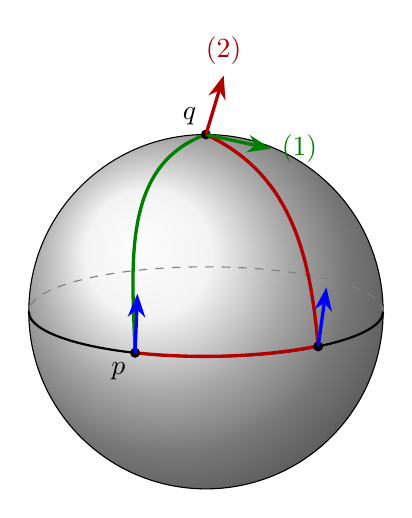
\begin{tikzpicture}[scale=1.5,>=Stealth]
  \shade[ball color=gray!12] (0,0) circle (1.5);
  \draw (0,0) circle (1.5);
  \draw[dashed,gray] (1.5,0) arc (0:180:1.5 and 0.38);
  \draw[thick] (-1.5,0) arc (180:360:1.5 and 0.38);
  \coordinate (q) at (0,1.5);
  \coordinate (p) at (-0.6,-0.348);
  \coordinate (r) at (0.95,-0.294);
  \draw[very thick,green!50!black] (p) to[out=92,in=200] (q);
  \draw[very thick,red!70!black] (p) arc (247:310:1.5 and 0.38);
  \draw[very thick,red!70!black] (r) to[out=95,in=-25] (q);
  \fill (p) circle (1.2pt); \node[below left] at (p) {$p$};
  \fill (r) circle (1.2pt);
  \fill (q) circle (1.2pt); \node[above left] at (q) {$q$};
  \draw[->,very thick,blue] (p) -- ++(0.02,0.5);
  \draw[->,very thick,blue] (r) -- ++(0.07,0.5);
  \draw[->,very thick,green!50!black] (q) -- ++(0.55,-0.12) node[right] {(1)};
  \draw[->,very thick,red!70!black] (q) -- ++(0.15,0.5) node[above] {(2)};
\end{tikzpicture}
\end{center}
This path dependence is precisely what the curvature tensor, introduced below, measures.
\end{carroll}


\item On the other hand, if we travel along the same curve between $p$ and $q$, but at a different rate (i.e.\ if we reparametrise the curve), the parallel-transported vector obtained at $q$ from a vector $A_0\in T_pM$ does not change. The reason is that under the reparametrisation $\gamma(\sigma(\sigma'))$ the differential equation of parallel transport is modified to
\[
  \frac{dA^\alpha}{d\sigma'}+\left.\Gamma^\alpha_{\mu\nu}\right|_\gamma A^\mu\frac{d\gamma^\nu}{d\sigma'}=\frac{dA^\alpha}{d\sigma'}+\left.\Gamma^\alpha_{\mu\nu}\right|_\gamma A^\mu(\sigma')\frac{d\gamma^\nu}{d\sigma}\frac{d\sigma}{d\sigma'}=\frac{d\sigma}{d\sigma'}\left(\frac{dA^\alpha}{d\sigma}+\left.\Gamma^\alpha_{\mu\nu}\right|_\gamma A^\mu\frac{d\gamma^\nu}{d\sigma}\right)
\]
so that if $A^\alpha(\sigma)$ is a solution of the parallel transport equation along the curve $\gamma(\sigma)$, then $A(\sigma(\sigma'))$ is the solution of the parallel transport equation along the reparametrised curve $\gamma(\sigma(\sigma'))$. The value of the field at each point of the curve is not modified.
\end{points}

\section{Autoparallel curves}

\begin{points}
\item In Euclidean space we have a set of very special curves: straight lines.

\item These curves are the only ones that have the following two properties.

(i) They minimise the distance between two given points,

(ii) The acceleration of the curve is proportional to the velocity.

\item To generalise these properties to differentiable manifolds we must be able either to have a notion of distance along a curve (property (i)) or to know what the acceleration is (property (ii)).

\item For the first we will need a metric, which we will introduce later, but for the second it is only necessary to have a connection.

\item Given a trajectory $\{x^\alpha(t)\}$ on a manifold, the velocity of the curve is simply the tangent vector to the trajectory
\[
  V^\alpha(t)=\frac{dx^\alpha(t)}{dt} .
\]
The acceleration in Euclidean space in Cartesian coordinates $\{X^\alpha\}$ is $a^\alpha=\frac{d^2X^\alpha(t)}{dt^2}$. However, this expression is no longer valid when we use coordinates other than Cartesian ones.

\item In non-Cartesian coordinates of Euclidean space the acceleration involves additional terms. For example, in polar coordinates in the plane, a trajectory $\rho(t),\theta(t)$ has acceleration
\[
  \vec a=\left(\ddot\rho-\rho\dot\theta^2\right)u_\rho+\left(\rho\ddot\theta+2\dot\rho\dot\theta\right)u_\theta
\]
where $\{u_\rho,u_\theta\}$ is the basis of unit vectors along the coordinate lines $\rho$ and $\theta$ respectively.

\item The reason for this behaviour under changes of coordinates is that the expression $\frac{d^2x^\alpha(t)}{dt^2}$ does not define the components of any tensor.

\item If we look at the terms appearing in the acceleration when we express it in polar coordinates, we observe that, in addition to the terms in second derivatives, there are terms quadratic in the first derivatives.

\item As we will see below, these terms correspond to the connection symbols. The reason why the acceleration in Cartesian coordinates is simply $\frac{d^2x^\alpha}{dt^2}$ is that Euclidean space can be endowed with a connection whose symbols vanish identically when expressed in Cartesian coordinates.

\item We can define the acceleration of a curve on an arbitrary manifold endowed with a covariant derivative in the following way. Let us suppose that we have extended the velocity vector of the curve $V^\alpha(t)$ to a velocity field $V^\alpha(x^\beta)$, in such a way that, evaluated along the curve, it satisfies
\[
  V^\alpha(x(t))=\frac{dx^\alpha(t)}{dt}=V^\alpha(t).
\]
To compute the second derivative $\frac{d^2x^\alpha}{dt^2}$ we use the chain rule, as we already did in the equation of autoparallel curves,
\[
  \frac{d^2x^\alpha(t)}{dt^2}=\frac{dx^\beta}{dt}\left.\frac{\partial V^\alpha}{\partial x^\beta}\right|_{x(t)}=\left.V^\beta\partial_\beta V^\alpha\right|_{x(t)}
\]

\item The term on the right is not a vector, but on a manifold with a connection we can replace the partial derivative by the covariant derivative, and the result will automatically be a vector.

\item We therefore define the acceleration of the curve $\{x^\alpha(t)\}$ as
\[
  a^\alpha(t)=V^\beta\nabla_\beta V^\alpha|_{x(t)},\qquad\text{where}\qquad V^\alpha(t)=\frac{dx^\alpha(t)}{dt}.
\]

\item The acceleration of the curve is also usually denoted by
\[
  a^\alpha=\frac{\nabla^2x^\alpha(t)}{dt^2}
\]
for the same reasons as those indicated above.

\item The explicit expression of the tensor $a^\alpha(t)$ in an arbitrary coordinate system $\{x^\alpha\}$ is
\[
  a^\alpha(t)=V^\beta\partial_\beta V^\alpha+\left.\Gamma^\alpha_{\beta\mu}\right|_{x(t)}V^\beta V^\mu=\frac{d^2x^\alpha(t)}{dt^2}+\left.\Gamma^\alpha_{\beta\mu}\right|_{x(t)}\frac{dx^\beta}{dt}\frac{dx^\mu}{dt}
\]
and we recover the property that the terms that must be added to the second derivatives are always quadratic in the velocities.

\item It is important to stress that, when the components $a^\alpha$ are given by this expression, the acceleration vector is
\[
  a=a^\alpha\partial_{x^\alpha} .
\]
This vector is expressed in the basis $\partial_{x^\alpha}$. If we change this basis (even without changing the coordinates), the components of $a^\alpha$ change.

\item For example, in the case of polar coordinates described above, the basis $\{u_\rho,u_\theta\}$ is made of unit vectors, which are different from the coordinate vectors $\{\partial_\theta,\partial_\phi\}$ (the two bases are proportional, but with a proportionality factor that is different at each point).

\item On manifolds on which we have defined a connection we can now generalise the property that defines straight lines as those curves whose acceleration is proportional to the velocity.

\item We define \textbf{autoparallel} curves as those curves $x^\alpha(t)$ satisfying
\[
  a^\alpha(t)\propto v^\alpha(t).
\]
If we call $b(t)$ the proportionality factor, we obtain that the autoparallel curves are those satisfying
\[
  a^\alpha(t)=b(t)v^\alpha(t)
\]
for some function $b(t)$. Explicitly, the following equation must be satisfied
\[
  \frac{d^2x^\alpha(t)}{dt^2}+\left.\Gamma^\alpha_{\beta\mu}\right|_{x(t)}\frac{dx^\beta}{dt}\frac{dx^\mu}{dt}=b(t)\frac{dx^\alpha}{dt}.
\]

\item If we know $b(t)$ explicitly, the autoparallel-curve equation is a second-order differential equation. Once an initial point $x^\alpha(t_0)$ and an initial velocity $v^\alpha(t_0)$ are fixed at an initial value of the parameter $t$, we have a unique solution $x^\alpha(t)$.

\item Autoparallel curves have the following property (exercise: prove it)
\end{points}

\textbf{Exercise 1.} \emph{For every autoparallel curve $x^\alpha(t)$ there exists a reparametrisation of the curve $x^\alpha(t(s))$ whose tangent vector
\[
  W^\alpha:=\frac{dx^\alpha}{ds}
\]
satisfies the autoparallel-curve equation with $b(s)=0$. That is, the acceleration of the curve vanishes:
\[
  W^\alpha\nabla_\alpha W^\beta=0.
\]
Moreover, the affine parameter is unique up to transformations $s'=a_0s+b_0$, with $a_0\neq0$, $b_0\in\R$.}

\begin{points}
\item In particular, the vector $W^\alpha$ satisfies the parallel transport equation along $x^\alpha(s)$. Hence the name autoparallel curve.
\end{points}

\section{Torsion and curvature}

\begin{points}
\item Every connection on a manifold has two associated tensors, torsion and curvature. Both encode important properties of the connection that defines them.

\item The first notion is that of torsion, which measures, among other things, whether the second covariant derivatives of a scalar function commute.

\item Let us consider a scalar function $f$ and a local coordinate system $\{x^\alpha\}$. The differential of $f$ is the 1-form $df=\partial_\alpha f\,dx^\alpha$.

\item The second covariant derivative of $f$ is (using the general expression for the covariant derivative of a 1-form)
\[
  \nabla_\beta\nabla_\alpha f=\partial_\beta(df_\alpha)-\Gamma^\mu_{\alpha\beta}df_\mu=\partial_\beta\partial_\alpha f-\Gamma^\mu_{\alpha\beta}\partial_\mu f .
\]

\item Therefore, the antisymmetric part of the second covariant derivative of a function $f$ is
\[
  \nabla_\alpha\nabla_\beta f-\nabla_\beta\nabla_\alpha f=\left(\Gamma^\mu_{\alpha\beta}-\Gamma^\mu_{\beta\alpha}\right)\nabla_\mu f .
\]

\item The left-hand side is a tensor, so the right-hand side must also be one. Consequently, although the connection symbols are not tensors, their antisymmetric part is.

\item This antisymmetric part defines the torsion tensor $T$ (note the position of the indices in the following expression)
\[
  T^\mu_{\alpha\beta}:=\Gamma^\mu_{\beta\alpha}-\Gamma^\mu_{\alpha\beta} .
\]

\item In terms of this tensor, the antisymmetrised covariant derivative of a function $f$ satisfies
\[
  \left(\nabla_\alpha\nabla_\beta-\nabla_\beta\nabla_\alpha\right)f=-T^\mu_{\alpha\beta}\partial_\mu f .
\]

\item This definition is valid in any coordinate system. We can also define the torsion tensor in an equivalent way without having to use coordinates:

\item The torsion tensor is a multilinear map that takes a pair of vector fields $X,Y$ and gives the field $T(X,Y)$ defined by
\[
  T(X,Y)=\nabla_XY-\nabla_YX-[X,Y].
\]

\item The antisymmetry property $T(X,Y)=-T(Y,X)$ is immediate from the definition.

\item To check that $T(X,Y)$ defines a tensor we must check that it is multilinear, i.e.\ that given any function $f$ we have $T(fX,Y)=fT(X,Y)$ and $T(X,fY)=fT(X,Y)$. Given the antisymmetry, it is enough to prove that $T(fX,Y)=fT(X,Y)$, which follows from
\begin{align*}
  T(fX,Y)&=\nabla_{fX}Y-\nabla_Y(fX)-[fX,Y]\\
  &=f\nabla_XY-f\nabla_YX-Y(f)X-f[X,Y]+Y(f)X\\
  &=f\left(\nabla_XY-\nabla_YX-[X,Y]\right)\\
  &=fT(X,Y).
\end{align*}

\item The components $T^\mu_{\alpha\beta}$ of the torsion tensor in a basis $e_\alpha$ are
\[
  T(e_\alpha,e_\beta)=T^\mu_{\alpha\beta}e_\mu
\]

\item If the basis is a coordinate basis, we recover the previous definition in terms of the difference of the connection symbols
\[
  T(\partial_\alpha,\partial_\beta)=\nabla_{\partial_\alpha}\partial_\beta-\nabla_{\partial_\beta}\partial_\alpha-[\partial_\alpha,\partial_\beta]=\Gamma^\mu_{\beta\alpha}\partial_\mu-\Gamma^\mu_{\alpha\beta}\partial_\mu=\left(\Gamma^\mu_{\beta\alpha}-\Gamma^\mu_{\alpha\beta}\right)\partial_\mu=T^\mu_{\alpha\beta}\partial_\mu .
\]

\item Second partial derivatives in $\R^n$ commute, so it will be natural to impose the condition that the torsion of the connection vanishes.

\item The second fundamental tensor that can be defined from the covariant derivative is the curvature of the connection.

\item The geometric idea of curvature is to measure the difference between a vector $w^\alpha$ at a point and its parallel transport along an infinitesimally small parallelogram with sides $u^\alpha$ and $v^\alpha$.

\begin{carroll}[: the infinitesimal loop]
Transporting $w$ around the small parallelogram spanned by $u$ and $v$ (first along $u$ and then along $v$, or first along $v$ and then along $u$) produces two vectors that differ, to lowest order, by an amount proportional to $w$, to $u$ and to $v$:
\[
  \delta w^\alpha\propto R^\alpha{}_{\beta\mu\nu}\,w^\beta u^\mu v^\nu ,
\]
as computed explicitly further below with coordinate lines. The antisymmetry $R^\alpha{}_{\beta\mu\nu}=-R^\alpha{}_{\beta\nu\mu}$ reflects the fact that going around the loop in the opposite sense changes the sign of $\delta w$.
\begin{center}
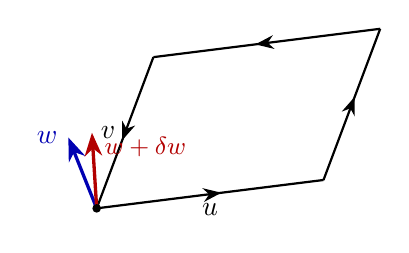
\begin{tikzpicture}[scale=1.2,>=Stealth]
  \coordinate (A) at (0,0); \coordinate (B) at (2.4,0.3); \coordinate (C) at (3.0,1.9); \coordinate (D) at (0.6,1.6);
  \draw[thick,->] (A) -- ($(A)!0.55!(B)$); \draw[thick] ($(A)!0.5!(B)$) -- (B);
  \draw[thick,->] (B) -- ($(B)!0.55!(C)$); \draw[thick] ($(B)!0.5!(C)$) -- (C);
  \draw[thick,->] (C) -- ($(C)!0.55!(D)$); \draw[thick] ($(C)!0.5!(D)$) -- (D);
  \draw[thick,->] (D) -- ($(D)!0.55!(A)$); \draw[thick] ($(D)!0.5!(A)$) -- (A);
  \node[below] at ($(A)!0.5!(B)$) {$u$};
  \node[left] at ($(A)!0.5!(D)$) {$v$};
  \draw[->,very thick,blue!70!black] (A) -- ++(-0.3,0.75) node[left] {$w$};
  \draw[->,very thick,red!70!black] (A) -- ++(-0.05,0.8);
  \node[red!70!black,right] at (-0.02,0.65) {\small $w+\delta w$};
  \fill (A) circle (1.3pt);
\end{tikzpicture}
\end{center}
\end{carroll}


\item To define it, it is convenient to try to generalise the previous construction of the torsion tensor. Instead of using second covariant derivatives of a function, we use second covariant derivatives of a vector field.

\item Given three vector fields $X,Y,Z$ we can define $\nabla_X\nabla_YZ-\nabla_Y\nabla_XZ$.

\item However, this construction does not define a tensor, since the operation is not multilinear in any of the three vectors.

\item Analogously to the case of torsion, it is possible to modify the expression by means of a Lie derivative in such a way that the result does define a tensor.

\item We introduce the curvature tensor $R(X,Y)Z$ as the operator that takes three vector fields $X,Y,Z$ and gives the vector
\[
  R(X,Y)Z=\nabla_X\nabla_YZ-\nabla_Y\nabla_XZ-\nabla_{[X,Y]}Z .
\]

\item By definition, this operator is antisymmetric in $X,Y$, i.e.
\[
  R(X,Y)Z=-R(Y,X)Z .
\]

\item To check that it defines a tensor, we must prove that it is multilinear in $X$, $Y$ and $Z$. Thanks to the antisymmetry in $X$, $Y$, it is enough to check $R(fX,Y)Z=fR(X,Y)Z$ and $R(X,Y)fZ=fR(X,Y)Z$, where $f$ is any scalar function.

\item We start with the first one
\begin{align*}
  R(fX,Y)Z&=\nabla_{fX}\nabla_YZ-\nabla_Y\nabla_{fX}Z-\nabla_{[fX,Y]}Z\\
  &=f\nabla_X\nabla_YZ-\nabla_Y(f\nabla_XZ)-\nabla_{f[X,Y]-Y(f)X}Z\\
  &=f\left(\nabla_X\nabla_YZ-\nabla_Y\nabla_XZ-\nabla_{[X,Y]}Z\right)-(\nabla_Yf)\nabla_XZ+Y(f)\nabla_XZ\\
  &=fR(X,Y)Z.
\end{align*}

\item For the second linearity property
\begin{align*}
  R(X,Y)fZ&=\nabla_X\nabla_Y(fZ)-\nabla_Y\nabla_X(fZ)-\nabla_{[X,Y]}(fZ)\\
  &=\nabla_X(Y(f)Z+f\nabla_YZ)-\nabla_Y(X(f)Z+f\nabla_XZ)-[X,Y](f)Z-f\nabla_{[X,Y]}Z\\
  &=X(Y(f))Z+Y(f)\nabla_XZ+X(f)\nabla_YZ+f\nabla_X\nabla_YZ\\
  &\quad-(Y(X(f))Z+X(f)\nabla_YZ+Y(f)\nabla_XZ+f\nabla_Y\nabla_XZ)-[X,Y](f)Z-f\nabla_{[X,Y]}Z\\
  &=\left(X(Y(f))-Y(X(f))-[X,Y](f)\right)Z+f\left(\nabla_X\nabla_YZ-\nabla_Y\nabla_XZ-\nabla_{[X,Y]}Z\right)\\
  &=fR(X,Y)Z.
\end{align*}

\item Therefore $R(X,Y)Z$ defines a tensor. Since it acts on three vectors and gives a vector, this operator defines a tensor that is 1 time contravariant and 3 times covariant.

\item The components $R^\alpha{}_{\beta\mu\nu}$ of this tensor in a basis $\{e_\alpha\}$ and its dual $\{\theta^\alpha\}$ are defined by (note the position of the indices)
\[
  R(e_\mu,e_\nu)e_\beta=R^\alpha{}_{\beta\mu\nu}e_\alpha\qquad\Longleftrightarrow\qquad R^\alpha{}_{\beta\mu\nu}=\theta^\alpha\left(R(e_\mu,e_\nu)e_\beta\right).
\]

\item From the antisymmetry of $R(X,Y)Z$ in $X,Y$ follows the antisymmetry property in the last two indices
\[
  R^\alpha{}_{\beta\mu\nu}=-R^\alpha{}_{\beta\nu\mu} .
\]

\item Since the curvature is defined from a connection, there must be an explicit expression for the curvature tensor in terms of the connection symbols.

\item Suppose that $e_\alpha=\partial_{x^\alpha}$ is a coordinate basis (so that $[e_\alpha,e_\beta]=0$). Recalling that the connection symbols in this basis are defined by
\[
  \nabla_{e_\nu}e_\beta=\Gamma^\alpha_{\beta\nu}e_\alpha
\]
we can compute the second covariant derivative
\begin{align*}
  \nabla_{e_\mu}\nabla_{e_\nu}e_\beta=\nabla_{e_\mu}\left(\Gamma^\alpha_{\beta\nu}e_\alpha\right)=e_\mu\left(\Gamma^\alpha_{\beta\nu}\right)e_\alpha+\Gamma^\alpha_{\beta\nu}\nabla_{e_\mu}e_\alpha&=\frac{\partial\Gamma^\alpha_{\beta\nu}}{\partial x^\mu}e_\alpha+\Gamma^\alpha_{\beta\nu}\Gamma^\gamma_{\alpha\mu}e_\gamma\\
  &=\left(\frac{\partial\Gamma^\alpha_{\beta\nu}}{\partial x^\mu}+\Gamma^\rho_{\beta\nu}\Gamma^\alpha_{\rho\mu}\right)e_\alpha
\end{align*}

\item Inserting into the definition of the curvature tensor,
\begin{align*}
  R^\alpha{}_{\beta\mu\nu}e_\alpha=R(e_\mu,e_\nu)e_\beta&=\nabla_{e_\mu}\nabla_{e_\nu}e_\beta-\nabla_{e_\nu}\nabla_{e_\mu}e_\beta-\nabla_{[e_\mu,e_\nu]}e_\beta=\nabla_{e_\mu}\nabla_{e_\nu}e_\beta-\nabla_{e_\nu}\nabla_{e_\mu}e_\beta\\
  &=\left(\frac{\partial\Gamma^\alpha_{\beta\nu}}{\partial x^\mu}-\frac{\partial\Gamma^\alpha_{\beta\mu}}{\partial x^\nu}+\Gamma^\alpha_{\rho\mu}\Gamma^\rho_{\beta\nu}-\Gamma^\alpha_{\rho\nu}\Gamma^\rho_{\beta\mu}\right)e_\alpha
\end{align*}
and we arrive at the following explicit expression in terms of the connection symbols
\[
  R^\alpha{}_{\beta\mu\nu}=\partial_\mu\Gamma^\alpha_{\beta\nu}-\partial_\nu\Gamma^\alpha_{\beta\mu}+\Gamma^\alpha_{\rho\mu}\Gamma^\rho_{\beta\nu}-\Gamma^\alpha_{\rho\nu}\Gamma^\rho_{\beta\mu} .
\]

\item As mentioned above, the curvature admits a geometric interpretation in terms of parallel transport along a parallelogram. The construction is as follows.

\item Let us consider a point $p\in M$ and a vector $Z$ in $T_pM$, and let us choose a coordinate system $x^\alpha$ containing $p$. By shifting the origin of the coordinates we can assume that the point $p$ has coordinates $x^\alpha(p)=0$.

\item Let us choose two independent coordinate lines passing through $p$. That is, we choose two different values of $\alpha$ and $\beta$ and consider the two curves $\gamma_\alpha(t)=(0,0,\cdots,t,\cdots0)$ and $\gamma_\beta(s)=(0,0,\cdots,s,\cdots0)$, where in the first curve $t$ is in the $\alpha$-th position and in the second $s$ is in the $\beta$-th position.

\item If we transport $Z$ parallelly along the curve $\gamma_\alpha$ we obtain a field $Z^\nu_1(t)$ along this curve that satisfies the equation
\[
  \frac{dZ^\nu_1(t)}{dt}+\left.\Gamma^\nu_{\mu\alpha}\right|_{\gamma_\alpha(t)}Z^\mu_1(t)=0 .
\]

\item For small values of $t$, the expression of the field $Z_1(t)$ is
\begin{equation}
  Z^\nu_1(t)=Z^\nu|_p-t\Gamma^\nu_{\mu\alpha}|_pZ^\mu|_p+O(t^2).
\end{equation}

\item From the point $\gamma_\alpha(t)$ we transport the vector $Z_1(t)$ parallelly along the curve $\gamma^t_\beta(s)$ defined by $x^\alpha=t$, $x^\beta=s$ and the rest of the coordinates equal to zero (the parameter of the curve is $s$, while $t$ is kept constant). Note that $\gamma^t_\beta(s=0)=\gamma_\alpha(t)$. The parallel transport equation is, in this case,
\[
  \frac{dZ^\nu_1(t;s)}{ds}+\left.\Gamma^\nu_{\mu\beta}\right|_{\gamma^t_\beta(s)}Z^\mu_1(t;s)=0 .
\]

\item For small values of $s$ we obtain
\[
  Z^\nu_1(t;s)=Z^\nu_1(t)-s\left.\Gamma^\nu_{\mu\beta}\right|_{\gamma_\alpha(t)}Z^\mu_1(t)+O(s^2).
\]

\item If the value of $t$ is also small, we can expand to first order in $t$ and use (4):
\begin{align*}
  Z^\nu_1(t;s)&=Z^\nu|_p-t\Gamma^\nu_{\mu\alpha}|_pZ^\mu|_p-s\left.\Gamma^\nu_{\mu\beta}\right|_{\gamma_\alpha(t)}\left(Z^\mu|_p-t\Gamma^\mu_{\gamma\alpha}Z^\gamma|_p+O(t^2)\right)+O(s^2)\\
  &=Z^\nu|_p-t\Gamma^\nu_{\mu\alpha}|_pZ^\mu|_p-s\left(\Gamma^\nu_{\mu\beta}|_p+t\partial_\alpha\Gamma^\nu_{\mu\beta}|_p\right)\left(Z^\mu|_p-t\Gamma^\mu_{\gamma\alpha}Z^\gamma|_p+O(t^2)\right)+O(s^2)\\
  &=Z^\nu|_p-t\Gamma^\nu_{\mu\alpha}|_pZ^\mu|_p-s\Gamma^\nu_{\mu\beta}|_pZ^\mu|_p-s\,t\left(\partial_\alpha\Gamma^\nu_{\mu\beta}Z^\mu|_p-\Gamma^\nu_{\mu\beta}\Gamma^\mu_{\gamma\alpha}Z^\gamma|_p\right)+O(t^2,s^2)\\
  &=Z^\nu|_p-t\Gamma^\nu_{\mu\alpha}|_pZ^\mu|_p-s\Gamma^\nu_{\mu\beta}|_pZ^\mu|_p-s\,t\left(\partial_\alpha\Gamma^\nu_{\mu\beta}-\Gamma^\nu_{\rho\beta}\Gamma^\rho_{\mu\alpha}\right)Z^\mu|_p+O(t^2,s^2).
\end{align*}
where in the second equality we have used a first-order Taylor expansion of $\Gamma^\nu_{\mu\beta}|_{\gamma_\alpha(t)}$.

\item We repeat the process but now moving first along the coordinate curve $x^\beta$ by an amount $s$ and then along the integral curve $x^\alpha$ by an amount $t$; we arrive at exactly the same point of space-time (with coordinates $x^\alpha=t$, $x^\beta=s$ and the rest of the coordinates zero). The transported vector $Z^\nu_2(s;t)$ in this case is obtained simply by interchanging $\alpha$ with $\beta$ and $t$ with $s$ in the previous expression. We obtain
\[
  Z^\nu_2(s;t)=Z^\nu|_p-s\Gamma^\nu_{\mu\beta}|_pZ^\mu|_p-t\Gamma^\nu_{\mu\alpha}|_pZ^\mu|_p-s\,t\left(\partial_\beta\Gamma^\nu_{\mu\alpha}-\Gamma^\nu_{\rho\alpha}\Gamma^\rho_{\mu\beta}\right)Z^\mu|_p+O(t^2,s^2).
\]

\item The difference between the two vectors evaluates the difference between transporting the vector along one path and transporting it along the other. The result is
\begin{align*}
  Z^\nu_2(s;t)-Z^\nu_1(t;s)&=s\,t\left(\partial_\alpha\Gamma^\nu_{\mu\beta}-\partial_\beta\Gamma^\nu_{\mu\alpha}-\Gamma^\nu_{\rho\beta}\Gamma^\rho_{\mu\alpha}+\Gamma^\nu_{\rho\alpha}\Gamma^\rho_{\mu\beta}\right)Z^\mu|_p+O(t^2,s^2)\\
  &=s\,t\,R^\nu{}_{\mu\alpha\beta}|_pZ^\mu|_p+O(t^2,s^2).
\end{align*}

\item Consequently, on a manifold with a connection whose curvature does not vanish, the notion of parallel transport is not absolute, but is associated with the path used for the transport. This property distinguishes these manifolds from Euclidean space.

\item In Euclidean space the manifold is $\R^n$. The Cartesian coordinates $\{X^\alpha\}$ define a basis of tangent vectors at each point that are parallel in the absolute sense, i.e.\ along any curve. In particular, $\partial_{X^\alpha}$ is parallel along the integral curve of $X^\beta$ and therefore
\[
  \nabla_{\partial_{X^\alpha}}\partial_{X^\beta}=0 .
\]
By the definition of the connection symbols we have $\Gamma^\alpha_{\beta\mu}=0$ in these coordinates. This connection of Euclidean space is called the \textbf{flat connection}. It follows from the definition that the curvature and the torsion of the flat connection vanish identically.

\item The following result is fundamental in differential geometry. It states that the only connection whose torsion and curvature vanish is the flat connection.
\end{points}

\textbf{Theorem 1.} \emph{Let $(M,\nabla)$ be a differentiable manifold with a connection $\nabla$. There exists a coordinate system $\{X^\alpha\}$ in a neighbourhood of each point $p\in M$ with the property that the connection symbols $\Gamma^\alpha_{\mu\nu}$ vanish in these coordinates if and only if the torsion and the curvature of $\nabla$ vanish identically.}

\begin{points}
\item From now on we shall assume that we have a differentiable manifold $M$ endowed with a connection $\nabla$ and that the torsion of $\nabla$ vanishes identically.

\item This means that in local coordinates $\{x^\alpha\}$ the connection symbols are symmetric, i.e.
\[
  \Gamma^\alpha_{\mu\nu}=\Gamma^\alpha_{\nu\mu} .
\]

\item In these circumstances, the definition of the curvature tensor implies the following formula, whose validity is independent of the coordinate system $\{x^\alpha\}$ being used. Let $V^\alpha$ be any vector field expressed in this coordinate system. Then
\[
  \nabla_\mu\nabla_\nu V^\alpha-\nabla_\nu\nabla_\mu V^\alpha=R^\alpha{}_{\beta\mu\nu}V^\beta
\]

\item This identity is known as the \textbf{Ricci identity}.

\item To prove it, we simply recall that the covariant derivative of a tensor $W^\alpha_\nu$ has components
\[
  \nabla_\mu W^\alpha_\nu=\partial_\mu W^\alpha_\nu+\Gamma^\alpha_{\gamma\mu}W^\gamma_\nu-\Gamma^\gamma_{\nu\mu}W^\alpha_\gamma
\]

\item Therefore, if the connection has no torsion, we obtain
\[
  \nabla_\mu W^\alpha_\nu-\nabla_\nu W^\alpha_\mu=\partial_\mu W^\alpha_\nu-\partial_\nu W^\alpha_\mu+\Gamma^\alpha_{\rho\mu}W^\rho_\nu-\Gamma^\alpha_{\rho\nu}W^\rho_\mu
\]

\item Particularising to $W^\alpha_\mu=\nabla_\mu V^\alpha$ and taking into account that the coordinate expression of $\nabla_\mu V^\alpha$ is
\[
  \nabla_\mu V^\alpha=\partial_\mu V^\alpha+\Gamma^\alpha_{\gamma\mu}V^\gamma
\]
we obtain
\begin{align*}
  \nabla_\mu\nabla_\nu V^\alpha-\nabla_\nu\nabla_\mu V^\alpha&=\partial_\mu\left(\partial_\nu V^\alpha+\Gamma^\alpha_{\gamma\nu}V^\gamma\right)-\partial_\nu\left(\partial_\mu V^\alpha+\Gamma^\alpha_{\gamma\mu}V^\gamma\right)\\
  &\quad+\Gamma^\alpha_{\rho\mu}\left(\partial_\nu V^\rho+\Gamma^\rho_{\gamma\nu}V^\gamma\right)-\Gamma^\alpha_{\rho\nu}\left(\partial_\mu V^\rho+\Gamma^\rho_{\gamma\mu}V^\gamma\right)\\
  &=\left(\partial_\mu\Gamma^\alpha_{\gamma\nu}-\partial_\nu\Gamma^\alpha_{\gamma\mu}+\Gamma^\alpha_{\rho\mu}\Gamma^\rho_{\gamma\nu}-\Gamma^\alpha_{\rho\nu}\Gamma^\rho_{\gamma\mu}\right)V^\gamma\\
  &=R^\alpha{}_{\gamma\mu\nu}V^\gamma
\end{align*}
where in the last equality we have used the symmetry of the partial derivatives and that of the connection symbols.

\item Note that in this calculation we have expanded first the outermost covariant derivative, since if we expanded first an inner covariant derivative we would encounter terms of the type $\nabla_\mu(\partial_\nu V^\alpha)$. These terms are not defined, since the object in parentheses is not a tensor and it makes no sense to compute its covariant derivative.

\item The Ricci identity can be generalised to connections with torsion, although the resulting expression is slightly more complicated.

\item The Ricci identity can also be generalised to tensors of arbitrary type ($p$ times contravariant and $q$ times covariant). The corresponding expression is
\[
  \left(\nabla_\mu\nabla_\nu-\nabla_\nu\nabla_\mu\right)T^{\alpha_1\cdots\alpha_p}_{\beta_1\cdots\beta_q}=\sum_{i=1}^pR^{\alpha_i}{}_{\rho\mu\nu}T^{\alpha_1\cdots\rho\cdots\alpha_p}_{\beta_1\cdots\beta_q}-\sum_{j=1}^qR^\rho{}_{\beta_j\mu\nu}T^{\alpha_1\cdots\alpha_p}_{\beta_1\cdots\rho\cdots\beta_q} .
\]

\item The curvature tensor is not only antisymmetric in its last two indices. It also satisfies the \textbf{first Bianchi identity}, which, in the case of a torsion-free connection, states that
\[
  R^\alpha{}_{\beta\mu\nu}+R^\alpha{}_{\mu\nu\beta}+R^\alpha{}_{\nu\beta\mu}=0 .
\]

\item We can prove it from the definition of the curvature tensor
\begin{align*}
  R(X,Y)Z+R(Y,Z)X+R(Z,X)Y&=\nabla_X\nabla_YZ-\nabla_Y\nabla_XZ-\nabla_{[X,Y]}Z\\
  &\quad+\nabla_Y\nabla_ZX-\nabla_Z\nabla_YX-\nabla_{[Y,Z]}X\\
  &\quad+\nabla_Z\nabla_XY-\nabla_X\nabla_ZY-\nabla_{[Z,X]}Y\\
  &=\nabla_X\left(\nabla_YZ-\nabla_ZY\right)+\nabla_Y\left(\nabla_ZX-\nabla_XZ\right)+\nabla_Z\left(\nabla_XY-\nabla_YX\right)\\
  &\quad-\nabla_{[X,Y]}Z-\nabla_{[Y,Z]}X-\nabla_{[Z,X]}Y.
\end{align*}

\item We use that the connection has no torsion, so that $\nabla_XY-\nabla_YX=[X,Y]$, and we obtain
\begin{align*}
  R(X,Y)Z+R(Y,Z)X+R(Z,X)Y&=\nabla_X[Y,Z]+\nabla_Y[Z,X]+\nabla_Z[X,Y]-\nabla_{[X,Y]}Z-\nabla_{[Y,Z]}X-\nabla_{[Z,X]}Y\\
  &=[X,[Y,Z]]+[Y,[Z,X]]+[Z,[X,Y]]=0
\end{align*}
where in the second equality we have used again that the connection has no torsion, and in the last equality we have used the Jacobi identity.

\item In addition to this algebraic property, the curvature tensor satisfies a differential identity known as the \textbf{second Bianchi identity}.
\[
  \nabla_\gamma R^\alpha{}_{\beta\mu\nu}+\nabla_\mu R^\alpha{}_{\beta\nu\gamma}+\nabla_\nu R^\alpha{}_{\beta\gamma\mu}=0 .
\]

\item Again, this identity is valid when the connection has no torsion. If the torsion does not vanish, the corresponding expression is somewhat more complicated.

\item We can prove this identity from the Ricci identity, which, let us recall, states
\[
  \left(\nabla_\mu\nabla_\nu-\nabla_\nu\nabla_\mu\right)V^\alpha=R^\alpha{}_{\beta\mu\nu}V^\beta .
\]

\item We take the covariant derivative in the direction $\nabla_\gamma$ and obtain
\[
  \nabla_\gamma\nabla_\mu\nabla_\nu V^\alpha-\nabla_\gamma\nabla_\nu\nabla_\mu V^\alpha=\left(\nabla_\gamma R^\alpha{}_{\beta\mu\nu}\right)V^\beta+R^\alpha{}_{\beta\mu\nu}\nabla_\gamma V^\beta
\]

\item If we add three copies of this equation, after permuting the indices as they appear in the expression of the second Bianchi identity, we obtain
\begin{align*}
  \left(\nabla_\gamma R^\alpha{}_{\beta\mu\nu}+\nabla_\mu R^\alpha{}_{\beta\nu\gamma}+\nabla_\nu R^\alpha{}_{\beta\gamma\mu}\right)V^\beta&=\nabla_\gamma\nabla_\mu\nabla_\nu V^\alpha-\nabla_\gamma\nabla_\nu\nabla_\mu V^\alpha+\nabla_\mu\nabla_\nu\nabla_\gamma V^\alpha-\nabla_\mu\nabla_\gamma\nabla_\nu V^\alpha\\
  &\quad+\nabla_\nu\nabla_\gamma\nabla_\mu V^\alpha-\nabla_\nu\nabla_\mu\nabla_\gamma V^\alpha-R^\alpha{}_{\beta\mu\nu}\nabla_\gamma V^\beta-R^\alpha{}_{\beta\nu\gamma}\nabla_\mu V^\beta-R^\alpha{}_{\beta\gamma\mu}\nabla_\nu V^\beta
\end{align*}

\item We now use the Ricci identity applied to $\nabla_\mu V^\alpha$, $\nabla_\nu V^\alpha$ and $\nabla_\gamma V^\alpha$ and obtain
\begin{align*}
  \left(\nabla_\gamma R^\alpha{}_{\beta\mu\nu}+\nabla_\mu R^\alpha{}_{\beta\nu\gamma}+\nabla_\nu R^\alpha{}_{\beta\gamma\mu}\right)V^\beta&=R^\alpha{}_{\rho\gamma\mu}\nabla_\nu V^\rho-R^\rho{}_{\nu\gamma\mu}\nabla_\rho V^\alpha+R^\alpha{}_{\rho\mu\nu}\nabla_\gamma V^\rho-R^\rho{}_{\gamma\mu\nu}\nabla_\rho V^\alpha\\
  &\quad+R^\alpha{}_{\rho\nu\gamma}\nabla_\mu V^\rho-R^\rho{}_{\mu\nu\gamma}\nabla_\rho V^\alpha-\left(R^\alpha{}_{\rho\mu\nu}\nabla_\gamma V^\rho+R^\alpha{}_{\rho\nu\gamma}\nabla_\mu V^\rho+R^\alpha{}_{\rho\gamma\mu}\nabla_\nu V^\rho\right)=\\
  &=-\left(R^\rho{}_{\nu\gamma\mu}+R^\rho{}_{\gamma\mu\nu}+R^\rho{}_{\mu\nu\gamma}\right)\nabla_\rho V^\alpha=0
\end{align*}
where in the last equality we have used the first Bianchi identity. Since $V^\beta$ is arbitrary, we conclude the validity of
\[
  \nabla_\gamma R^\alpha{}_{\beta\mu\nu}+\nabla_\mu R^\alpha{}_{\beta\nu\gamma}+\nabla_\nu R^\alpha{}_{\beta\gamma\mu}=0 .
\]
\end{points}

\section{(Pseudo-)Riemannian manifolds}

\begin{points}
\item To be able to define distances on a differentiable manifold we need a metric.
\end{points}

\textbf{Definition 1.} \emph{A metric on a differentiable manifold $M$ is a symmetric ($g(X,Y)=g(Y,X)$) and non-degenerate 2-covariant tensor $g$, i.e.\ such that at each point $p\in M$ the following property holds:}
\[
  g|_p(X,Y)=0\quad\forall Y\in T_pM\qquad\Longrightarrow\qquad X=0 .
\]

\begin{points}
\item Given two vectors $X,Y\in T_pM$, the quantity $g|_p(X,Y)$ defines the \textbf{scalar product} of the two vectors.

\item When $g(X,Y)=0$ is satisfied we say that $X$ and $Y$ are \textbf{orthogonal}. Therefore, the non-degeneracy condition means that there is no vector orthogonal to all the others, except the zero vector.

\item In a basis $\{e_\alpha\}$ the components of $g$ are $g_{\alpha\beta}$, and the scalar product of two vectors $X=X^\alpha e_\alpha$ and $Y=Y^\alpha e_\alpha$ can be computed by
\[
  g(X,Y)=g_{\alpha\beta}X^\alpha Y^\beta .
\]

\item The condition that $g$ is a symmetric tensor is
\[
  g_{\alpha\beta}=g_{\beta\alpha}
\]
and the non-degeneracy condition is
\[
  g_{\alpha\beta}V^\beta=0\qquad\Longleftrightarrow\qquad V^\beta=0 .
\]

\item If we regard $g_{\alpha\beta}$ as an $n\times n$ square matrix (where $n$ is the dimension of the manifold), the non-degeneracy condition simply states that the matrix $g_{\alpha\beta}$ is invertible. We denote the components of the inverse matrix with the indices up, i.e.\ we define $g^{\alpha\beta}$ by the equation
\[
  g^{\alpha\mu}g_{\mu\beta}=\delta^\alpha_\beta .
\]

\item We can introduce a contravariant tensor $g^\sharp$ whose components in the basis $\{\theta^\alpha\}$ dual to $\{e_\alpha\}$ are $g^{\sharp\alpha\beta}=g^{\alpha\beta}$. This tensor is known as the \textbf{contravariant metric} (or inverse metric).

\item Given two 1-forms $\omega=\omega_\alpha\theta^\alpha$ and $\Omega=\Omega_\alpha\theta^\alpha$, the scalar product of $\omega$ and $\Omega$ is defined by $g^\sharp(\omega,\Omega)$ or, in components,
\[
  g^{\alpha\beta}\omega_\alpha\Omega_\beta .
\]

\item Since the inverse of a symmetric matrix is also symmetric, the contravariant metric is a symmetric tensor $g^\sharp(\omega,\Omega)=g^\sharp(\Omega,\omega)$.

\item Since $g$ is a symmetric tensor, we can write its decomposition in the basis $\{\theta^\alpha\}$ in the following way
\[
  g=g_{\alpha\beta}\theta^\alpha\otimes\theta^\beta=\frac12g_{\alpha\beta}\theta^\alpha\otimes\theta^\beta+\frac12g_{\beta\alpha}\theta^\beta\otimes\theta^\alpha=\frac12g_{\alpha\beta}\left(\theta^\alpha\otimes\theta^\beta+\theta^\beta\otimes\theta^\alpha\right).
\]

\item It is usual to write $\theta^\alpha\theta^\beta:=\frac12\left(\theta^\alpha\otimes\theta^\beta+\theta^\beta\otimes\theta^\alpha\right)$, so that we can express the metric in the form
\[
  g=g_{\alpha\beta}\theta^\alpha\theta^\beta .
\]

\item In particular, if we use a coordinate basis $\theta^\alpha=dx^\alpha$, the metric is defined by the so-called \textbf{line element} $ds^2$, defined by
\[
  ds^2=g_{\alpha\beta}dx^\alpha dx^\beta .
\]

\item $ds^2$ is simply another way of writing the tensor $g$, so we can also express it in an arbitrary cobasis, $ds^2=g_{\alpha\beta}\theta^\alpha\theta^\beta$.

\item At each point $p\in M$, the line element $ds^2$ defines a quadratic form. An important result of algebra states that every quadratic form admits a basis that diagonalises it and in which, moreover, the terms on the diagonal consist only of $+1$, $-1$ or $0$. There are multiple bases that diagonalise a quadratic form, but the number of $+1$, $-1$ and $0$ appearing in the canonical form is independent of the basis (Sylvester's law of inertia).

\item Since metrics are non-degenerate, they cannot contain any zero in their canonical form. Therefore, there exists a basis of vectors $\{e_\alpha\}$ in $T_pM$, whose dual basis we call $\{\theta^\alpha\}$, in which $ds^2|_p$ takes the form
\[
  ds^2|_p=\underbrace{-(\theta^1)^2-(\theta^2)^2-\cdots-(\theta^{p})^2}_{p\text{ terms}}+\underbrace{(\theta^{p+1})^2+(\theta^{p+2})^2+\cdots+(\theta^n)^2}_{n-p\text{ terms}} .
\]

\item In matrix form, the components of the metric in this basis are
\[
  g_{\alpha\beta}=\mathrm{diag}\{-1,\cdots,-1,+1,\cdots,+1\}.
\]

\item The basis $\{e_\alpha\}$ is called orthonormal. The reason for this name is that any two different vectors of the basis are orthogonal to each other and, moreover, the scalar product of a basis vector with itself is $-1$ or $+1$.

\item The number $n-2p$, which coincides with the sum of the $-1$ and $+1$ in the diagonal expression of the metric (since $n-2p=(n-p)1+p(-1)$), is called the \textbf{signature}. The collection of numbers $\{-1,\cdots-1,1,\cdots1\}$ appearing in the canonical form of the metric is also called the \textbf{signature}.

\item A metric is called \textbf{Riemannian} if the signature is $n$ (or $-n$, although this form is used less). From a geometric point of view, this condition states that any non-zero vector $V\in T_pM$ has a positive scalar product with itself:
\[
  g(V,V)>0\qquad\text{for every }V\in T_pM\text{ with }V\neq0 .
\]
In general, the \textbf{squared norm} of a vector $V$ with respect to a metric $g$ is defined as $V^2|_g:=g(V,V)$. For an arbitrary metric, this squared norm can be zero (even if the vector does not vanish) or negative. If there is no possibility of confusion, the squared norm can be denoted simply by $V^2$.

\item In a Riemannian metric, the squared norm of a vector is positive except when the vector vanishes. In these circumstances we can define the norm of $V$ as $|V|:=\sqrt{V^2}$.

\item A metric is called \textbf{Lorentzian} if it has signature $n-2$ or, equivalently, $\{-1,+1,\cdots+1\}$ (the opposite signature $\{+1,-1,-1,\cdots,-1\}$ is also used).

\item In general, a metric $g$ with an arbitrary signature is called pseudo-Riemannian. A manifold $M$ endowed with a pseudo-Riemannian metric $g$ is called a \textbf{pseudo-Riemannian manifold} and is denoted by $(M,g)$.

\item If the metric of $(M,g)$ is Riemannian, we call $(M,g)$ a \textbf{Riemannian manifold}, and if the signature is Lorentzian, $(M,g)$ is called a \textbf{Lorentzian manifold}.

\item Given a pseudo-Riemannian manifold $(M,g)$, we can define a canonical isomorphism between vectors and covectors, which is called the musical isomorphism (because of the flat symbol that is usually used to denote it). The more prosaic name of ``lowering an index'' is also used. The intrinsic definition of this operation is
\[
  \begin{array}{rcl}
  \flat:T_pM&\longrightarrow&T^\star_pM\\
  V&\longrightarrow&V_\flat:\left\{\begin{array}{rcl}T_pM&\longrightarrow&\R\\ W&\longrightarrow&g(V,W).\end{array}\right.
  \end{array}
\]

\item In any basis $\{e_\alpha\}$ and its dual $\{\theta^\alpha\}$, the components of $V_\flat$ are $V_{\flat\alpha}:=g_{\alpha\beta}V^\beta$. In index notation, the position of the indices already identifies whether we are dealing with a vector or a covector, so it is not necessary to use the symbol $\flat$ and we can simply write $V_\alpha=g_{\alpha\beta}V^\beta$; hence the name ``lowering the index'' that this operation also receives.

\item Analogously, we can define the operation of raising the index of a covector $\omega_\alpha$ and define the vector
\[
  \omega^\alpha=g^{\alpha\beta}\omega_\beta .
\]

\item The operations of raising and lowering indices are inverse to each other. Indeed, if we raise the index of $V_\flat$ we obtain
\[
  g^{\alpha\beta}V_\beta=g^{\alpha\beta}g_{\beta\mu}V^\mu=\delta^\alpha_\mu V^\mu=V^\alpha
\]
and we recover the original vector.

\item Given any tensor $T^{\alpha_1\cdots\alpha_p}_{\beta_1\cdots\beta_q}$, we can raise and lower any of its indices. If we want to use the same symbol $T$ for all the tensors constructed in this way, it is necessary to place each of the indices in a different vertical slot, so as to know without ambiguity which index we have raised and lowered. If we write the tensor $T$ in the form $T^{\alpha_1\cdots\alpha_p}{}_{\beta_1\cdots\beta_q}$ and, for example, we lower the first index and raise the $(p+1)$-th one, we obtain
\[
  T_{\alpha_1}{}^{\alpha_2\cdots\alpha_p\beta_1}{}_{\beta_2\cdots\beta_q}
\]
and there is no ambiguity in the meaning.
\end{points}

\section{Levi-Civita connection}

\begin{points}
\item Let us suppose that we have a manifold $M$ on which a connection $\nabla$ and a metric $g$ are defined. In that case we have a notion of parallel transport along curves, as well as a notion of scalar product.

\item We can ask whether it is possible to relate both concepts. A natural compatibility consists in studying whether it is possible to make the parallel transport of vectors keep their scalar product constant. Let us consider two vectors $X(\sigma)$, $Y(\sigma)$ parallelly propagated along a curve $\gamma(\sigma)$ with tangent vector $u(\sigma)$. Therefore the equations $\nabla_uX=\nabla_uY=0$ are satisfied.

\item We can compute the directional derivative of $g(X,Y)$ (which is a scalar function of $\sigma$ along the curve), i.e.
\begin{align*}
  \frac{dg(X,Y)}{d\sigma}&=u^\alpha\partial_\alpha(g(X,Y))=u^\alpha\nabla_\alpha(g(X,Y))\\
  &=\left(u^\alpha\nabla_\alpha g\right)(X,Y)+g(u^\alpha\nabla_\alpha X,Y)+g(X,u^\alpha\nabla_\alpha Y)=\left(u^\alpha\nabla_\alpha g\right)(X,Y).
\end{align*}

\item We conclude that the scalar product $g(X,Y)$ is constant along any curve if and only if $\nabla_\alpha g_{\mu\nu}=0$.

\item Given a metric $g$, the connections $\nabla$ satisfying $\nabla g=0$ are called \textbf{compatible with the metric}, or simply \textbf{metric}.

\item A fundamental theorem of differential geometry states that, given a metric $g$, there exists a unique connection $\nabla$ that is at the same time metric and whose torsion vanishes (i.e.\ which is torsion-free).
\end{points}

\textbf{Theorem 2} (Levi-Civita)\textbf{.} \emph{Given a pseudo-Riemannian manifold $(M,g)$, there exists a unique connection $\nabla$ satisfying: (i) the torsion vanishes and (ii) it is compatible with the metric, $\nabla g=0$. This connection is called the Levi-Civita connection.}

\begin{points}
\item We shall give a constructive proof that will allow us to obtain an explicit expression for the symbols of the Levi-Civita connection $\Gamma^\alpha_{\beta\mu}$ in any coordinate basis. These connection symbols are known as \textbf{Christoffel symbols}.

\item The absence of torsion imposes the condition $\Gamma^\alpha_{\beta\mu}=\Gamma^\alpha_{\mu\beta}$, and compatibility with the metric imposes the condition
\begin{equation}
  \nabla_\alpha g_{\beta\gamma}=\partial_\alpha g_{\beta\gamma}-\Gamma^\mu_{\beta\alpha}g_{\mu\gamma}-\Gamma^\mu_{\gamma\alpha}g_{\beta\mu}=0 .
\end{equation}
Note that this expression includes a large number of conditions, since the indices $\alpha$, $\beta$ and $\gamma$ are free. At the same time, the equation involves a large number of unknowns (each of the terms $\Gamma^\mu_{\beta\alpha}$). The idea is to combine all these equations algebraically to obtain the solution.

\item We permute the indices $\alpha\beta\gamma$ cyclically and obtain three sets of equations
\begin{align*}
  \partial_\alpha g_{\beta\gamma}&=\Gamma^\mu_{\beta\alpha}g_{\mu\gamma}+\Gamma^\mu_{\gamma\alpha}g_{\beta\mu},\\
  \partial_\beta g_{\gamma\alpha}&=\Gamma^\mu_{\gamma\beta}g_{\mu\alpha}+\Gamma^\mu_{\alpha\beta}g_{\gamma\mu},\\
  \partial_\gamma g_{\alpha\beta}&=\Gamma^\mu_{\alpha\gamma}g_{\mu\beta}+\Gamma^\mu_{\beta\gamma}g_{\alpha\mu}.
\end{align*}

\item If we add the first two equations and subtract the third, four of the terms on the right cancel (since the connection is symmetric) and the other two simply add up. We obtain
\[
  \partial_\alpha g_{\beta\gamma}+\partial_\beta g_{\alpha\gamma}-\partial_\gamma g_{\alpha\beta}=2\Gamma^\mu_{\alpha\beta}g_{\mu\gamma}
\]
We invert the metric $g_{\mu\gamma}$ (or, more precisely, we multiply by $g^{\gamma\nu}$) and obtain
\begin{equation}
  \Gamma^\nu_{\alpha\beta}=\frac12g^{\nu\gamma}\left(\partial_\alpha g_{\beta\gamma}+\partial_\beta g_{\alpha\gamma}-\partial_\gamma g_{\alpha\beta}\right).
\end{equation}
Since we have obtained an explicit and unique expression, we can conclude that, if the Levi-Civita connection does exist, it must necessarily have this form.

\item To check that the Christoffel symbols (6) do satisfy all the equations, we simply observe that they are symmetric in $\alpha\beta$ (so that they define a torsion-free connection) and that, if we substitute them into (5), we obtain $\nabla_\alpha g_{\beta\gamma}=0$.

\item The Levi-Civita connection also satisfies
\[
  \nabla_\alpha g^{\mu\nu}=0 .
\]
To prove it, we use the property that any connection has (regardless of whether it has torsion or not, or whether it is metric or not) that the covariant derivative of the identity always vanishes identically. The identity $I$ is the 1-covariant, 1-contravariant tensor defined by $I(V)=V$ for any vector $V\in T_pM$. If we apply a covariant derivative to this expression we obtain
\[
  \nabla_XV=\nabla_XI(V)=(\nabla_XI)(V)+I(\nabla_XV)=(\nabla_XI)(V)+\nabla_XV\qquad\Longleftrightarrow\qquad\nabla_XI=0,
\]

\item We can also prove this property by a calculation in a coordinate basis $\{\partial_{x^\alpha}\}$. In this basis the tensor $I^\alpha{}_\beta$ is simply the Kronecker delta $I^\alpha{}_\beta=\delta^\alpha{}_\beta$. We compute its covariant derivative
\[
  \nabla_\mu\delta^\alpha{}_\beta=\partial_\mu\delta^\alpha{}_\beta+\Gamma^\alpha_{\rho\mu}\delta^\rho{}_\beta-\Gamma^\rho_{\beta\mu}\delta^\alpha{}_\rho=\Gamma^\alpha_{\beta\mu}-\Gamma^\alpha_{\beta\mu}=0 .
\]

\item To compute $\nabla_\nu g^{\alpha\beta}$ we recall the definition $g^{\alpha\beta}g_{\beta\mu}=\delta^\alpha_\mu$. Taking the covariant derivative of this equality we arrive at
\[
  0=\nabla_\nu\delta^\alpha_\mu=\nabla_\nu(g^{\alpha\beta}g_{\beta\mu})=(\nabla_\nu g^{\alpha\beta})g_{\beta\mu}+g^{\alpha\beta}\nabla_\mu g_{\beta\mu}=(\nabla_\nu g^{\alpha\beta})g_{\beta\mu}\qquad\Longrightarrow\qquad\nabla_\nu g^{\alpha\beta}=0
\]
\end{points}


\section{Riemann, Ricci and Einstein tensors.}

\begin{points}
\item The curvature tensor $R^\alpha{}_{\beta\gamma\mu}$ of the Levi-Civita connection is called the \textbf{Riemann tensor}.

\item Since we have a metric that allows us to lower and raise indices, we can define the totally covariant Riemann tensor (or simply ``with all indices down'') by
\[
  R_{\alpha\beta\mu\nu}:=g_{\alpha\gamma}R^\gamma{}_{\beta\mu\nu} .
\]

\item The Riemann tensor has the following algebraic properties
\begin{align*}
  R_{\alpha\beta\mu\nu}&=-R_{\alpha\beta\nu\mu},\\
  R_{\alpha\beta\mu\nu}&=-R_{\beta\alpha\mu\nu},\\
  R_{\alpha\beta\mu\nu}+R_{\alpha\mu\nu\beta}+R_{\alpha\nu\beta\mu}&=0\\
  R_{\alpha\beta\mu\nu}&=R_{\mu\nu\alpha\beta}.
\end{align*}

\item The first one corresponds simply to the antisymmetry in the last two indices that every curvature tensor has, and the third one is the first Bianchi identity.

\item The second one is a consequence of the Ricci identity applied to the metric $g$. Using that $\nabla_\alpha g_{\mu\nu}=0$ (and therefore its second covariant derivatives also vanish),
\[
  \nabla_\alpha\nabla_\beta g_{\mu\nu}-\nabla_\beta\nabla_\alpha g_{\mu\nu}=-R^\rho{}_{\mu\alpha\beta}g_{\rho\nu}-R^\rho{}_{\nu\alpha\beta}g_{\mu\rho}=-R_{\nu\mu\alpha\beta}-R_{\mu\nu\alpha\beta}=0
\]

\item The fourth algebraic property $R_{\alpha\beta\mu\nu}=R_{\mu\nu\alpha\beta}$ is a consequence of the three previous ones.
\end{points}

\textbf{Exercise 2.} \emph{Prove that the Riemann tensor satisfies $R_{\alpha\beta\mu\nu}=R_{\mu\nu\alpha\beta}$ starting from the antisymmetry in the first two indices, in the last two indices and from the first Bianchi identity.}

\begin{points}
\item From the Riemann tensor we can define other curvature tensors by taking traces with the metric $g$.

\item Given a tensor $T^{\alpha_1\cdots\alpha_p}{}_{\beta_1\cdots\beta_q}$, $p$ times contravariant and $q$ times covariant, we can contract one contravariant and one covariant index (for example $\alpha_1$ and $\beta_1$) and obtain a tensor $(p-1)$ times contravariant and $(q-1)$ times covariant, with components
\[
  T^{\alpha_2\cdots\alpha_p}{}_{\beta_2\cdots\beta_q}:=T^{\alpha_1\cdots\alpha_p}{}_{\alpha_1\cdots\beta_q}
\]

\item Two contravariant indices can also be contracted, for example $\alpha_1$ and $\alpha_p$, with the metric $g$, defining a tensor $(p-2)$ times contravariant and $q$ times covariant by
\[
  T^{\alpha_2\cdots\alpha_{p-1}}{}_{\beta_1\cdots\beta_q}:=g_{\alpha_1\alpha_p}T^{\alpha_1\cdots\alpha_p}{}_{\beta_1\cdots\beta_q}
\]

\item This operation can be done with any pair of contravariant indices (naturally, in general the result depends on the indices chosen to perform the contraction).

\item Analogously, we can contract pairs of covariant indices with the contravariant metric. For example, if we contract the indices $\beta_1$ and $\beta_q$ we obtain
\[
  T^{\alpha_1\cdots\alpha_p}{}_{\beta_2\cdots\beta_{q-1}}:=g^{\beta_1\beta_q}T^{\alpha_1\cdots\alpha_p}{}_{\beta_1\cdots\beta_q}
\]

\item An important algebraic property is that, if a tensor $T^{\alpha_1\cdots\alpha_p}{}_{\beta_1\cdots\beta_q}$ is antisymmetric in a pair of indices, the tensor obtained by contracting them vanishes identically.

\item More generally, the contraction of a symmetric tensor $S^{\alpha\beta}$ and an antisymmetric tensor $A_{\alpha\beta}$ vanishes identically (exercise: prove it).

\item We now define the tensors that can be obtained by contracting the Riemann tensor.

\item Given the algebraic properties of this tensor, it is only possible to construct a single independent trace.

\item We define the Ricci tensor by
\[
  R_{\alpha\beta}=R^\mu{}_{\alpha\mu\beta} .
\]

\item From the properties of the Riemann tensor it follows that the Ricci tensor is symmetric.
\[
  R_{\alpha\beta}=R^\mu{}_{\alpha\mu\beta}=g^{\mu\nu}R_{\mu\alpha\nu\beta}=g^{\mu\nu}R_{\nu\beta\mu\alpha}=R_{\beta\alpha} .
\]

\item The number of independent components of a symmetric tensor on a manifold of dimension $n$ is $\frac{n(n+1)}{2}$. In dimension four, the number of independent components of the Ricci tensor is 10.

\item The rest of the traces of the Riemann tensor either vanish (for example when contracting the first two or the last two indices) or give tensors that can be written directly in terms of the Ricci tensor.

\item From the Ricci tensor we can define a single trace. The result is a scalar function known as the curvature scalar (or Ricci scalar), defined by
\[
  R=g^{\alpha\beta}R_{\alpha\beta} .
\]

\item From the Ricci tensor and the curvature scalar one defines a fundamental tensor in general relativity, the so-called Einstein tensor
\[
  G_{\alpha\beta}:=R_{\alpha\beta}-\frac12Rg_{\alpha\beta} .
\]

\item This tensor is symmetric. If the dimension $n$ is at least three, the Einstein tensor contains the same information as the Ricci tensor. Indeed, the trace of the metric tensor $g$ is a constant function whose value is the dimension of the manifold
\[
  g^{\alpha\beta}g_{\alpha\beta}=\delta^\alpha{}_\alpha=n
\]
since $\delta$ is the identity matrix and its trace is directly $n$.

\item Taking the trace of the Einstein tensor,
\[
  G:=G_{\alpha\beta}g^{\alpha\beta}=R-\frac12Rn=\frac{2-n}{2}R .
\]

\item Therefore, the Ricci tensor can be written in terms of the Einstein tensor by
\[
  R_{\alpha\beta}=G_{\alpha\beta}+\frac12Rg_{\alpha\beta}=G_{\alpha\beta}-\frac{1}{n-2}Gg_{\alpha\beta} .
\]

\item The fundamental importance of the Einstein tensor is that it satisfies an identity called the ``conservation identity''
\[
  \nabla_\alpha G^{\alpha\beta}=0 .
\]
This expression is satisfied identically for any metric and its corresponding Levi-Civita connection and Einstein tensor. It can be proved directly from the second Bianchi identity by taking two traces, as follows:
\[
  \nabla_\alpha R_{\beta\gamma\mu\nu}+\nabla_\mu R_{\beta\gamma\nu\alpha}+\nabla_\nu R_{\beta\gamma\alpha\mu}=0
\]
We first contract with $g^{\beta\mu}$ and use that $\nabla_\alpha g^{\beta\mu}=0$, so that the metric can go through the covariant derivative
\[
  \nabla_\alpha(g^{\beta\mu}R_{\beta\gamma\mu\nu})+\nabla_\mu R^\mu{}_{\gamma\nu\alpha}+\nabla_\nu(g^{\beta\mu}R_{\beta\gamma\alpha\mu})=\nabla_\alpha R_{\gamma\nu}+\nabla_\mu R^\mu{}_{\gamma\nu\alpha}-\nabla_\nu R_{\gamma\alpha}=0
\]

\item We now contract with $g^{\alpha\gamma}$ and arrive at
\[
  \nabla_\alpha R^\alpha{}_\nu+\nabla_\mu R^\mu{}_\nu-\nabla_\nu R=\nabla_\alpha\left(2R^\alpha{}_\nu-R\delta^\alpha{}_\nu\right)=2\nabla_\alpha G^\alpha{}_\nu=0
\]
\end{points}

\section{Geodesics}

\begin{points}
\item Let us consider a Riemannian manifold $(M,g)$. Given a curve $\gamma(\sigma)$ between two points $p=\gamma(\sigma_0)$ and $q=\gamma(\sigma_1)$, we can define the \textbf{length} between $p$ and $q$ along the curve $\gamma(\sigma)$ by the following expression
\[
  L=\int_{\sigma_0}^{\sigma_1}\sqrt{g(\dot\gamma,\dot\gamma)}d\sigma
\]
where $\dot\gamma$ is the tangent vector to the curve.

\item To motivate this definition, we can use a local coordinate system $\{x^\alpha\}$ in which the curve has the form $x^\alpha(\sigma)$. The tangent vector is
\[
  \dot\gamma=\frac{dx^\alpha}{d\sigma}\partial_{x^\alpha}
\]
so that we have
\[
  g(\dot\gamma,\dot\gamma)=g_{\alpha\beta}|_{x(\sigma)}\frac{dx^\alpha}{d\sigma}\frac{dx^\beta}{d\sigma} .
\]

\item If we substitute it into the expression for $L$ we arrive at
\[
  L=\int_{\sigma_0}^{\sigma_1}\sqrt{g_{\alpha\beta}|_{x(\sigma)}\frac{dx^\alpha}{d\sigma}\frac{dx^\beta}{d\sigma}}d\sigma=\int_\gamma\sqrt{g_{\alpha\beta}|_{x(\sigma)}dx^\alpha dx^\beta}=\int_\gamma\sqrt{ds^2}=\int_\gamma ds
\]
so that the length is indeed the sum (integral) of the infinitesimal distance elements $ds$ along the curve.

\item This expression shows that the distance between two points along a curve does not depend on the way we parametrise the curve. It depends only on the path we use to go from $p$ to $q$.

\item Given two points $p,q$, we can consider all the curves $\gamma$ going from $p$ to $q$ and compute the distance between $p$ and $q$ along each of these curves. In this way we define a functional on the set of curves, which we call the \textbf{distance functional}.

\item We call \textbf{geodesic} any curve that makes the distance functional take an extremal (or ``stationary'') value.

\item To find the equation satisfied by geodesics, we must obtain the Euler--Lagrange equations of the functional $L[\gamma]$. This calculation presents a complication due to the fact that the functional is invariant under reparametrisations, so that the differential equation we obtain can never have a unique solution (if a curve $x^\alpha(\sigma)$ satisfies the Euler--Lagrange equation, then any reparametrisation $x^\alpha(\sigma(\sigma'))$ must also satisfy that same equation).

\item There are several ways of dealing with this difficulty. A particularly simple one is to choose for each curve a parametrisation (which turns out to be unique) satisfying the following three conditions
\[
  x^\alpha(\sigma=0)=p,\qquad x^\alpha(\sigma=1)=q,\qquad\frac{dx^\alpha}{d\sigma}\text{ has constant norm}
\]

\item That is, we impose the condition that we move with a ``speed'' of constant modulus along the curve, and that we leave at $\sigma=0$ and arrive at $\sigma=1$. Physically it is clear (and easy to prove) that this parametrisation exists and is unique.

\item With these restrictions, the functional is
\[
  L[\gamma]=\int_{\sigma=0}^{\sigma=1}\sqrt{g_{\alpha\beta}|_{x(\sigma)}\frac{dx^\alpha}{d\sigma}\frac{dx^\beta}{d\sigma}}d\sigma .
\]

\item Although the quantity $g_{\alpha\beta}(x(\sigma))\frac{dx^\alpha}{d\sigma}\frac{dx^\beta}{d\sigma}$ is independent of $\sigma$, its value is different for each curve.

\item We can write the Euler--Lagrange equations of this functional
\[
  \frac{d}{d\sigma}\left(\frac{\partial\mathcal L}{\partial\dot x^\alpha}\right)=\frac{\partial\mathcal L}{\partial x^\alpha}
\]
where
\[
  \mathcal L(x^\alpha,\dot x^\alpha)=\sqrt{g_{\alpha\beta}|_{x(\sigma)}\dot x^\alpha\dot x^\beta}
\]
is the Lagrangian of the functional $L$. We evaluate the derivatives
\[
  \frac{d}{d\sigma}\left(\frac{g_{\alpha\beta}\dot x^\beta}{\sqrt{g_{\mu\nu}|_{x(\sigma)}\dot x^\mu\dot x^\nu}}\right)=\frac{(\partial_\alpha g_{\beta\gamma})\dot x^\gamma}{2\sqrt{g_{\mu\nu}|_{x(\sigma)}\dot x^\mu\dot x^\nu}} .
\]

\item We can now use the fact that $\sqrt{g_{\alpha\beta}|_{x(\sigma)}\dot x^\alpha\dot x^\beta}$ is constant along the curve, so that it can be taken out of the derivative on the left and cancel the corresponding factor on the right. We obtain
\[
  \frac{d}{d\sigma}\left(g_{\alpha\beta}\dot x^\beta\right)=\frac12(\partial_\alpha g_{\beta\gamma})\dot x^\beta\dot x^\gamma
\]

\item We evaluate the total derivative on the left
\begin{align*}
  (\partial_\gamma g_{\alpha\beta})\dot x^\gamma\dot x^\beta+g_{\alpha\beta}\ddot x^\beta&=\frac12(\partial_\alpha g_{\beta\gamma})\dot x^\beta\dot x^\gamma\qquad\Longleftrightarrow\\
  \ddot x^\mu&=g^{\mu\alpha}\left(\frac12(\partial_\alpha g_{\beta\gamma})\dot x^\beta\dot x^\gamma-\partial_\gamma g_{\alpha\beta}\dot x^\gamma\dot x^\beta\right)\\
  &=g^{\mu\alpha}\left(\frac12(\partial_\alpha g_{\beta\gamma})\dot x^\beta\dot x^\gamma-\frac12\partial_\gamma g_{\alpha\beta}\dot x^\gamma\dot x^\beta-\frac12\partial_\beta g_{\alpha\gamma}\dot x^\gamma\dot x^\beta\right)\\
  &=-\Gamma^\mu_{\beta\gamma}\dot x^\beta\dot x^\gamma .
\end{align*}

\item Therefore the Euler--Lagrange equations are
\[
  \frac{d^2x^\mu}{d\sigma^2}+\left.\Gamma^\mu_{\beta\gamma}\right|_{x(\sigma)}\frac{dx^\beta}{d\sigma}\frac{dx^\gamma}{d\sigma}=0
\]
which can be written in covariant form (as it must be, since we have not imposed any condition on the coordinates)
\[
  u^\alpha\nabla_\alpha u^\beta=0\qquad\text{where}\qquad u^\alpha=\frac{dx^\alpha}{d\sigma} .
\]

\item We have obtained that the geodesic equation on a Riemannian manifold coincides with the equation of the autoparallel curves with zero acceleration of its Levi-Civita connection. If we had not imposed the condition that the velocity of the curve has constant modulus, we would have obtained (with a bit more work) the equation of the autoparallel curves $a^\alpha=b(\sigma)u^\alpha$.

\item Therefore, on any Riemannian manifold, geodesics are at the same time the curves that make the distance between two points extremal and the curves whose acceleration is parallel to the velocity, as happens in the case of straight lines in Euclidean space.

\item A self-consistency check of the previous derivation is the following exercise.
\end{points}

\textbf{Exercise 3.} \emph{Prove that any curve satisfying $a^\alpha:=u^\mu\nabla_\mu u^\alpha=0$, where $u^\alpha$ is the tangent vector to the curve, has the property that
\[
  g_{\alpha\beta}u^\alpha u^\beta=\text{const}.
\]
Conversely, if a curve satisfies $a^\alpha=bu^\alpha$ and the tangent vector has constant modulus different from zero along the curve, then necessarily $b=0$ and the equation $a^\alpha=0$ is satisfied.}

\begin{points}
\item We call \textbf{geodesic} any curve $x^\alpha(\sigma)$ satisfying the autoparallel-curve equation $a^\alpha=bu^\alpha$. In the case in which $a^\alpha=0$ is satisfied, we say that the curve is an \textbf{affinely parametrised geodesic}.

\item These names are not universal; there are authors who prefer to call the former \textbf{pregeodesics} and to reserve the name \textbf{geodesics} for the latter.

\item Given any curve $\gamma(\sigma)$ on a Riemannian manifold, we can always find a parametrisation $\sigma(s)$ such that the tangent vector to the curve in the new parametrisation is unitary
\[
  g\left(\frac{d\gamma}{ds},\frac{d\gamma}{ds}\right)=1
\]
This parameter is called the \textbf{arc length}, and it is unique except for the possibility of choosing its origin arbitrarily.

\item On a geodesic, the arc-length parameter is always an affine parameter.
\end{points}

\section{Geodesics in pseudo-Riemannian manifolds.}

\begin{points}
\item On pseudo-Riemannian manifolds a vector can have a negative squared norm, so that the square root $\sqrt{g_{\alpha\beta}|_{x(\sigma)}\dot x^\alpha\dot x^\beta}$ may cease to make sense as a real quantity.

\item This difficulty can be solved by defining the following functional on curves
\[
  \mathcal F[\gamma]=\int_\gamma\sqrt{|g(\dot\gamma,\dot\gamma)|}d\sigma .
\]

\item This functional is differentiable on curves whose tangent vector satisfies
\[
  g(\dot\gamma,\dot\gamma)\neq0
\]
and, if we compute its corresponding Euler--Lagrange equations, we obtain the equation of the autoparallel curves
\begin{equation}
  u^\alpha\nabla_\alpha u^\beta=b(\sigma)u^\alpha,\qquad u^\alpha=\frac{dx^\alpha}{d\sigma} .
\end{equation}
When we use the affine parametrisation, in which $g_{\alpha\beta}u^\alpha u^\beta=\text{const}$ is satisfied,
\begin{equation}
  u^\alpha\nabla_\alpha u^\beta=0\qquad u^\alpha=\frac{dx^\alpha}{d\sigma} .
\end{equation}

\item Analogously to the previous case, a curve satisfying (7) is a geodesic of the pseudo-Riemannian manifold $(M,g)$, and a curve satisfying (8) is, by definition, an affinely parametrised geodesic of $(M,g)$.

\item It is important to stress that the equation of affinely parametrised geodesics (8) also turns out to be the Euler--Lagrange equation of another functional on curves, called the \textbf{energy of the curve}.

\item This alternative functional is defined by
\[
  E[\gamma]=\frac12\int_\gamma g(\dot\gamma,\dot\gamma)d\sigma
\]
and it makes sense even when the tangent vector to the curve has zero squared modulus.

\item Its expression in coordinates is
\[
  E(x^\alpha(\sigma))=\frac12\int_{\sigma=\sigma_0}^{\sigma=\sigma_1}g_{\alpha\beta}|_{x(\sigma)}\frac{dx^\alpha}{d\sigma}\frac{dx^\beta}{d\sigma} .
\]

\item By means of a calculation analogous to the one done for the Euler--Lagrange equations of the length of a curve $L[\gamma]$, it is easy to conclude that the Euler--Lagrange equations of $E[\gamma]$ are precisely the equations of affinely parametrised geodesics.

\item The energy functional is not invariant under reparametrisations. In the case of geodesic curves, the energy functional automatically selects an affine parameter, so that the acceleration of the curve vanishes.

\item An efficient way of computing the Christoffel symbols of a pseudo-Riemannian metric $g$ consists in writing the energy functional of that metric and computing the Euler--Lagrange equations explicitly. From the expression
\[
  \frac{d^2x^\alpha}{d\sigma^2}+\Gamma^\alpha_{\beta\mu}\frac{dx^\beta}{d\sigma}\frac{dx^\mu}{d\sigma}=0
\]
and from the fact that the Christoffel symbols are symmetric (i.e.\ $\Gamma^\alpha_{\beta\mu}=\Gamma^\alpha_{\mu\beta}$ is satisfied), the explicit expressions of all the Christoffel symbols of the metric can be extracted directly.
\end{points}

\begin{carroll}[: example --- the two-sphere]
Let us apply the method of the energy functional to the two-sphere of radius $a$, with metric
\[
  ds^2=a^2\left(d\theta^2+\sin^2\theta\,d\phi^2\right).
\]
The energy functional has Lagrangian $\frac12a^2(\dot\theta^2+\sin^2\theta\,\dot\phi^2)$, and its Euler--Lagrange equations are
\[
  \ddot\theta-\sin\theta\cos\theta\,\dot\phi^2=0,\qquad\ddot\phi+2\cot\theta\,\dot\theta\dot\phi=0 .
\]
Comparing with $\ddot x^\alpha+\Gamma^\alpha_{\beta\mu}\dot x^\beta\dot x^\mu=0$ (and remembering that a crossed term $\dot\theta\dot\phi$ appears twice in the sum), the only non-vanishing Christoffel symbols are
\[
  \Gamma^\theta_{\phi\phi}=-\sin\theta\cos\theta,\qquad\Gamma^\phi_{\theta\phi}=\Gamma^\phi_{\phi\theta}=\cot\theta .
\]
With $R^\alpha{}_{\beta\mu\nu}=\partial_\mu\Gamma^\alpha_{\beta\nu}-\partial_\nu\Gamma^\alpha_{\beta\mu}+\Gamma^\alpha_{\rho\mu}\Gamma^\rho_{\beta\nu}-\Gamma^\alpha_{\rho\nu}\Gamma^\rho_{\beta\mu}$,
\[
  R^\theta{}_{\phi\theta\phi}=\partial_\theta\Gamma^\theta_{\phi\phi}-\Gamma^\theta_{\phi\phi}\Gamma^\phi_{\phi\theta}=-(\cos^2\theta-\sin^2\theta)+\sin\theta\cos\theta\cot\theta=\sin^2\theta .
\]
In two dimensions this is the only independent component (the general count of independent components of the Riemann tensor in dimension $n$ is $\frac{n^2(n^2-1)}{12}$: 1 for $n=2$, 6 for $n=3$, 20 for $n=4$). Lowering the index, $R_{\theta\phi\theta\phi}=a^2\sin^2\theta$. The Ricci tensor and the curvature scalar are
\[
  R_{\theta\theta}=1,\qquad R_{\phi\phi}=\sin^2\theta,\qquad R_{\theta\phi}=0,\qquad R=g^{\theta\theta}R_{\theta\theta}+g^{\phi\phi}R_{\phi\phi}=\frac{2}{a^2}.
\]
The curvature scalar is positive and constant (the sphere is homogeneous), and it becomes smaller for larger spheres, as expected. (For a flat plane in polar coordinates, $ds^2=dr^2+r^2d\phi^2$, the Christoffel symbols $\Gamma^r_{\phi\phi}=-r$, $\Gamma^\phi_{r\phi}=1/r$ do not vanish, but the Riemann tensor does: non-vanishing connection symbols do not imply curvature.)
\end{carroll}









\end{document}
